
%
%	Appendix
%

\section{Other distributions}\label{App_Other}
\Headerfooter{Other distributions}





\subsection{Simulation}\label{App_Simula}
\vs\hs
Other distributions related to Section~\ref{Section_Simula} are summarized here.

\begin{figure}[H]
	\centering
	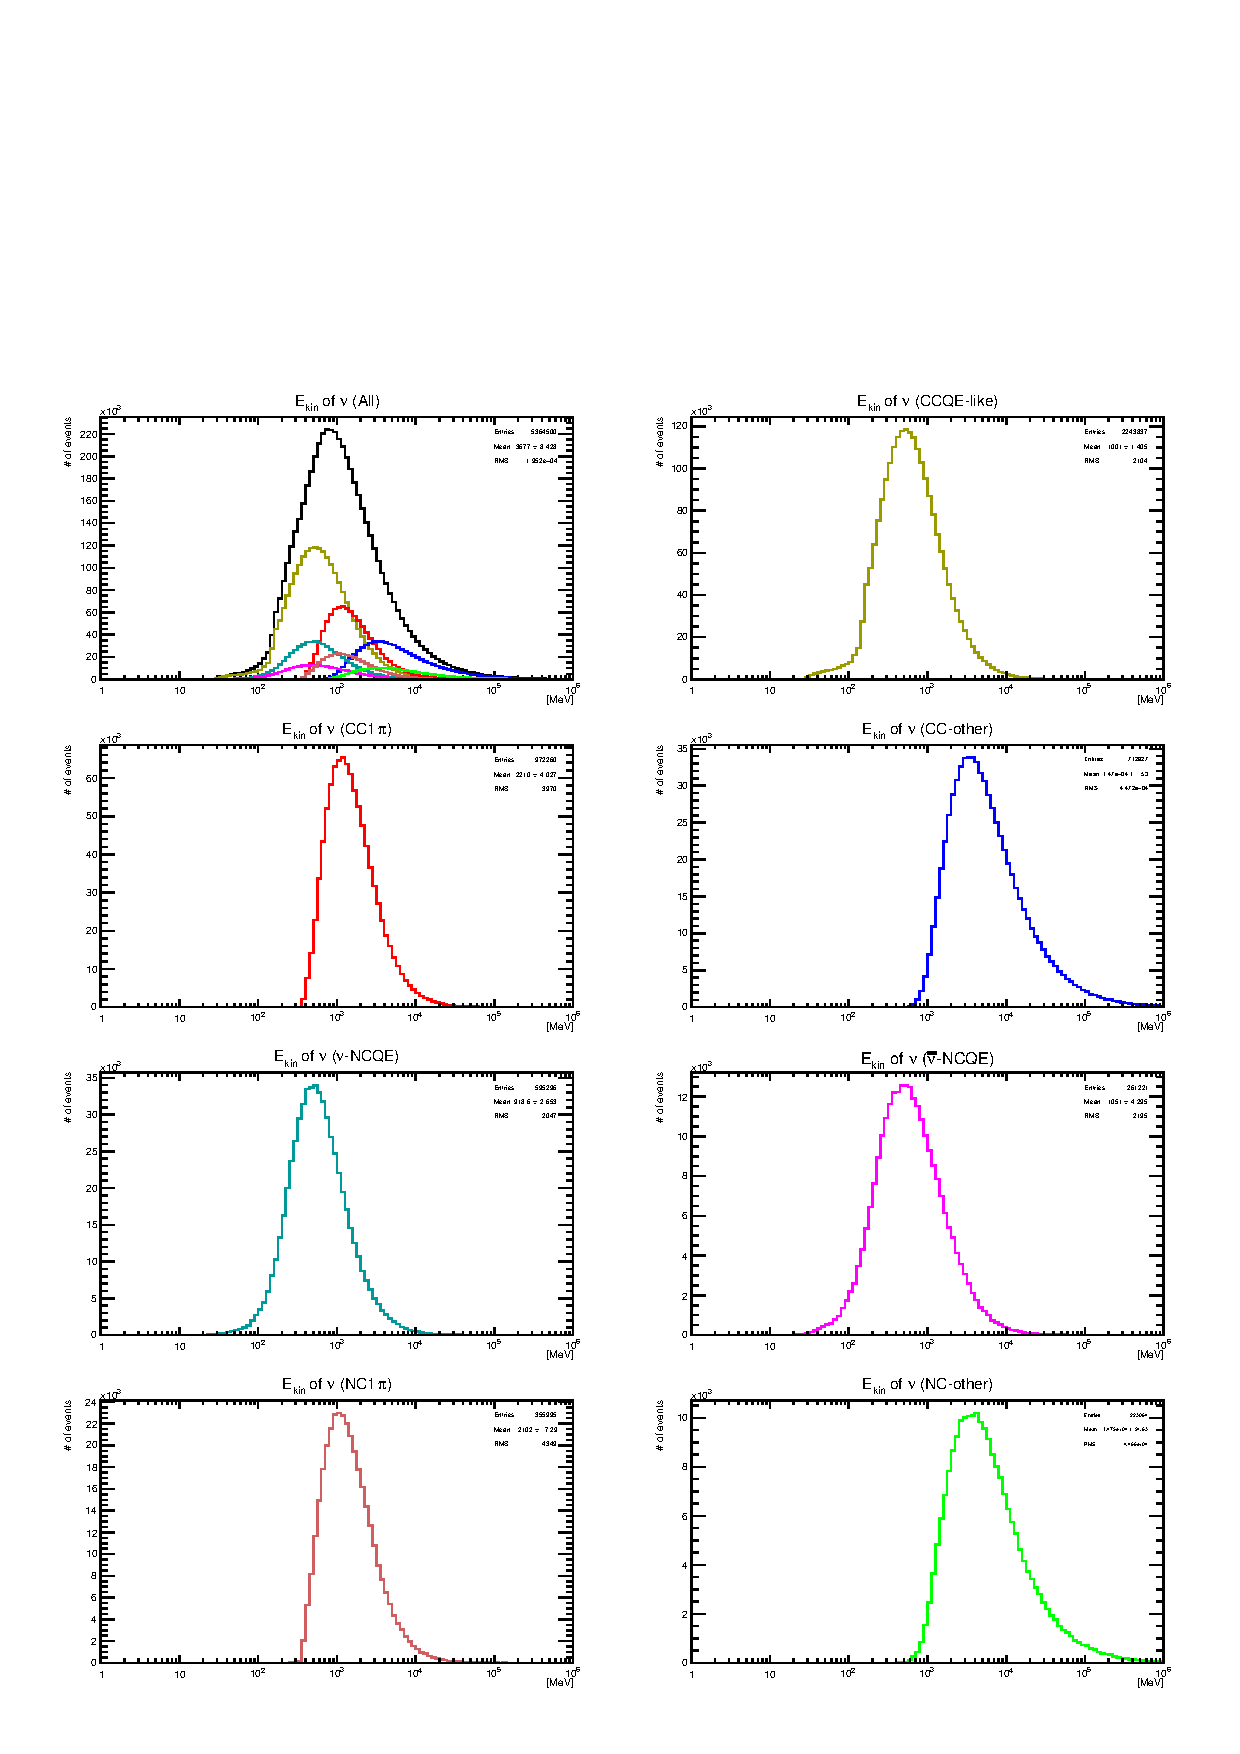
\includegraphics[width=16cm]{PDF/NEUT/s1_2_official/gamma/LogEneNeu}
	\caption[Energy of atmospheric neutrinos that induced neutrino-nucleus interactions]{
	Energy of atmospheric neutrinos that induced neutrino-nucleus interactions.
	These figures were made using 500 years' worth of atmospheric neutrino events.
	}\label{gammaLogEneNeu}
\end{figure}

\begin{figure}[h]
	\centering
	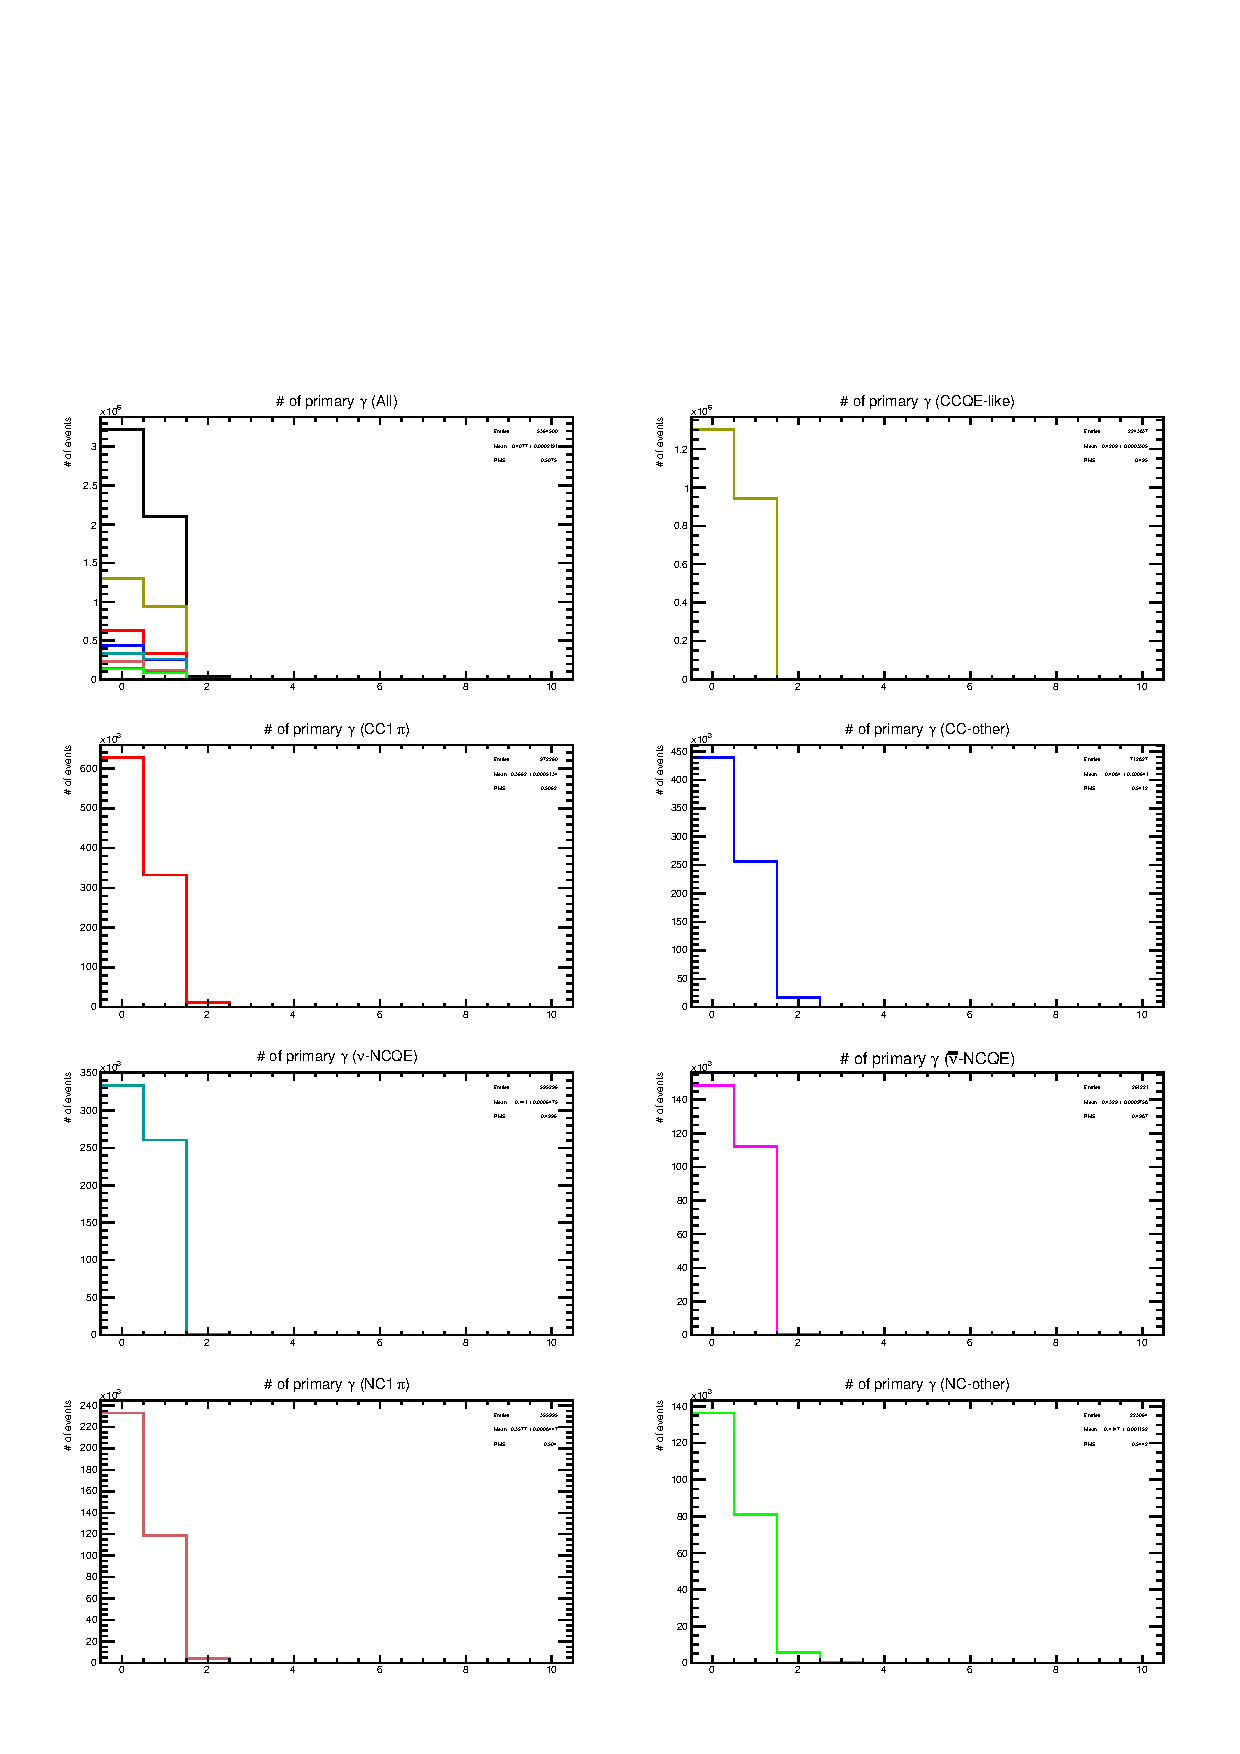
\includegraphics[width=16cm]{PDF/NEUT/s1_2_official/gamma/NumPri}
	\caption[The number of gamma-rays generated by neutrino-nucleus interactions]{
	The number of gamma-rays generated by neutrino-nucleus interactions.
	These figures were made using 500 years' worth of atmospheric neutrino events.
	}\label{gammaNumPri}
\end{figure}

\begin{figure}[h]
	\centering
	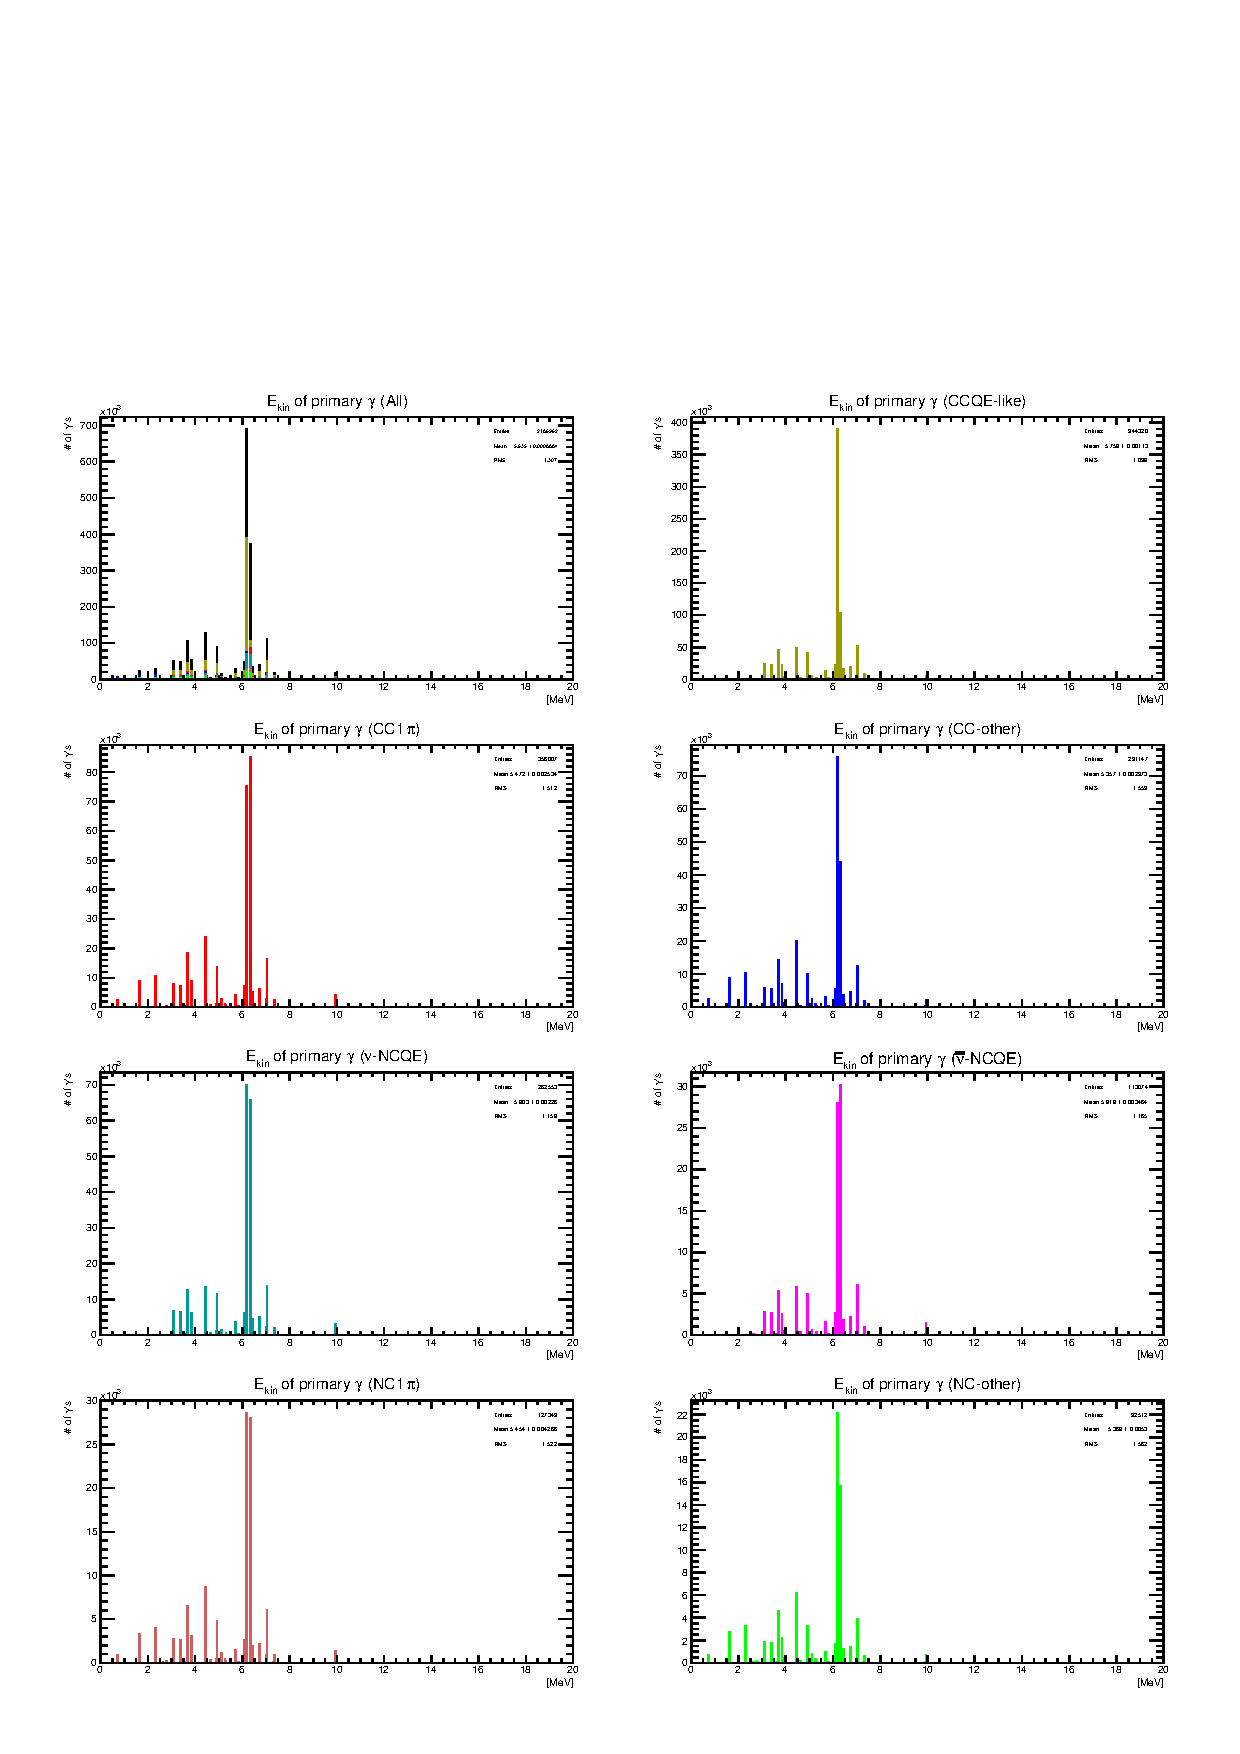
\includegraphics[width=16cm]{PDF/NEUT/s1_2_official/gamma/EnePri}
	\caption[Energy of gamma-rays generated by neutrino-nucleus interactions]{
	Energy of gamma-rays generated by neutrino-nucleus interactions.
	These figures were made using 500 years' worth of atmospheric neutrino events.
	}\label{gammaEnePri}
\end{figure}

\begin{figure}[h]
	\centering
	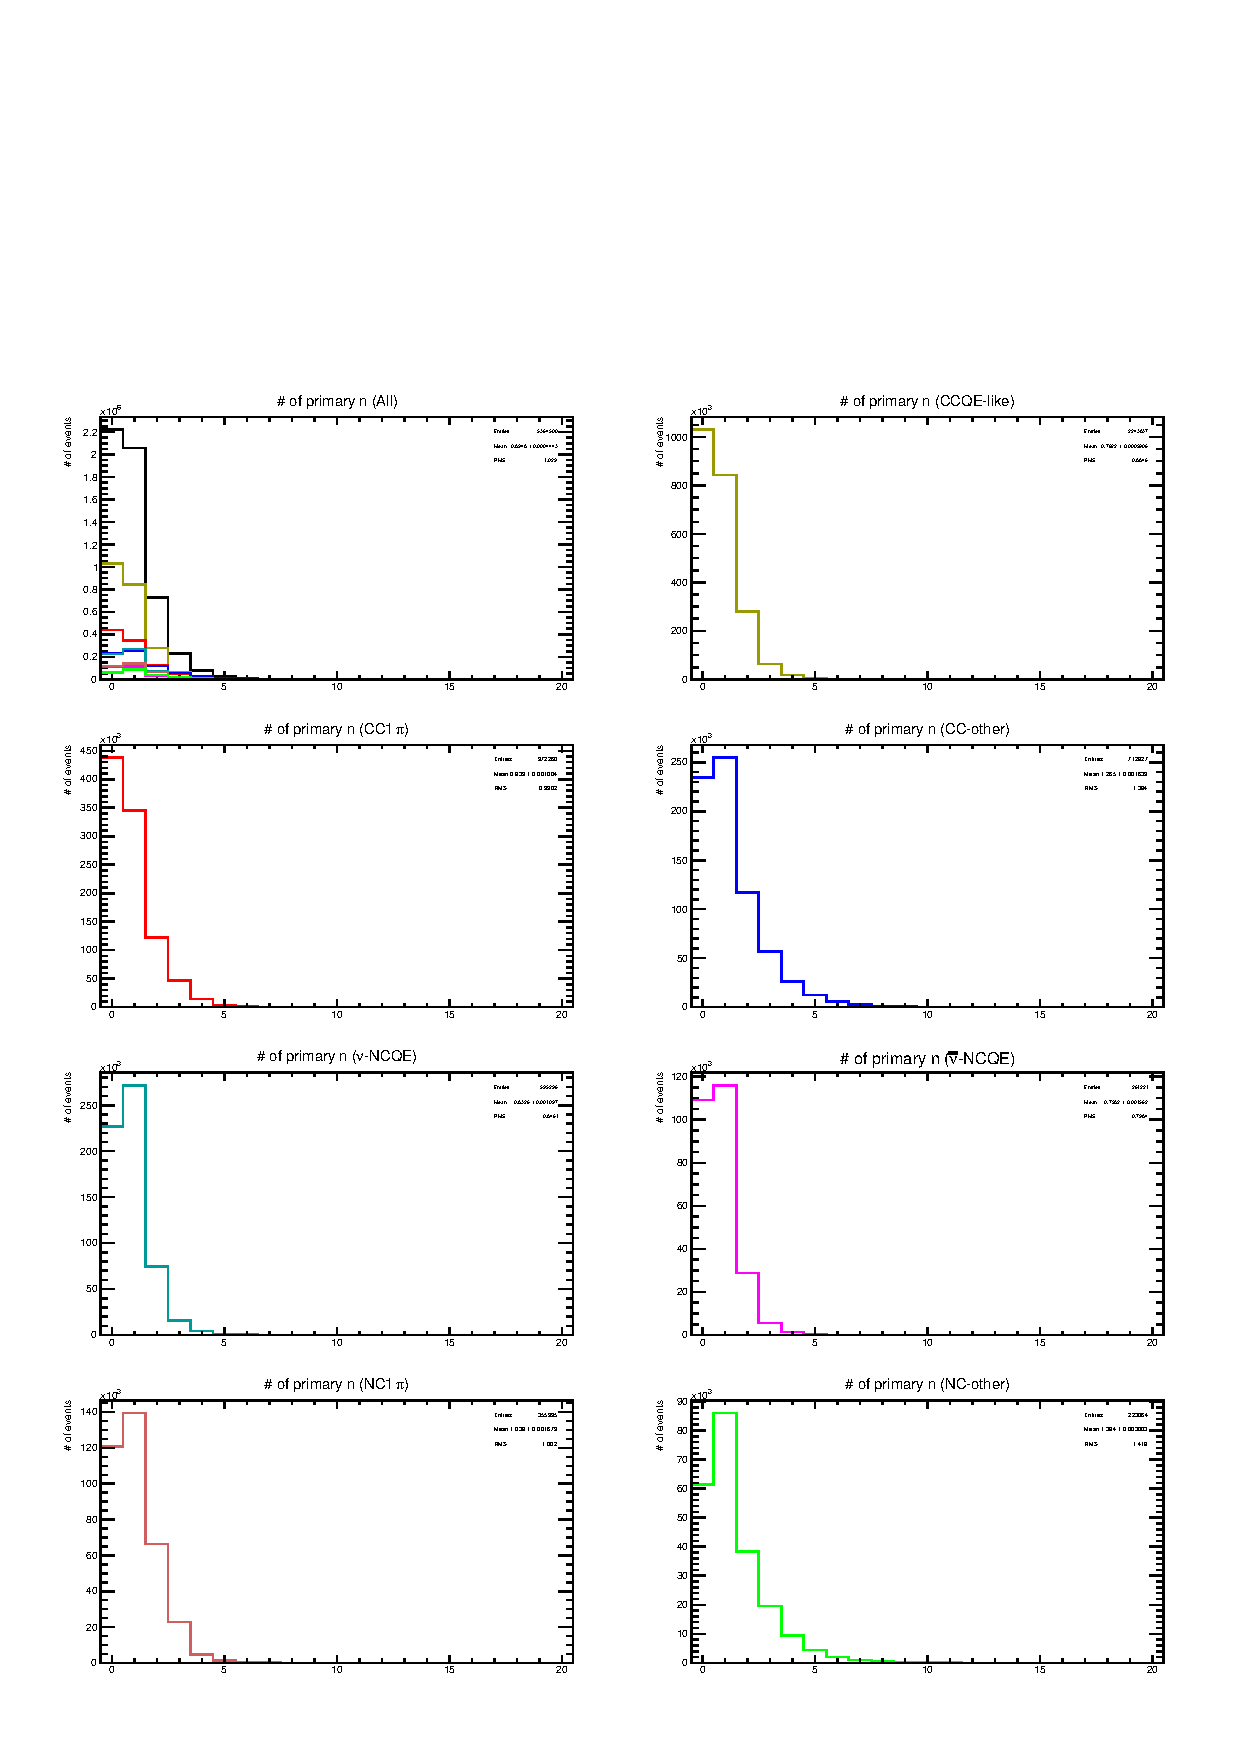
\includegraphics[width=16cm]{PDF/NEUT/s1_2_official/neutron/NumPri}
	\caption[The number of neutrons generated by neutrino-nucleus interactions]{
	The number of neutrons generated by neutrino-nucleus interactions.
	These figures were made using 500 years' worth of atmospheric neutrino events.
	}\label{neutronNumPri}
\end{figure}

\begin{figure}[h]
	\centering
	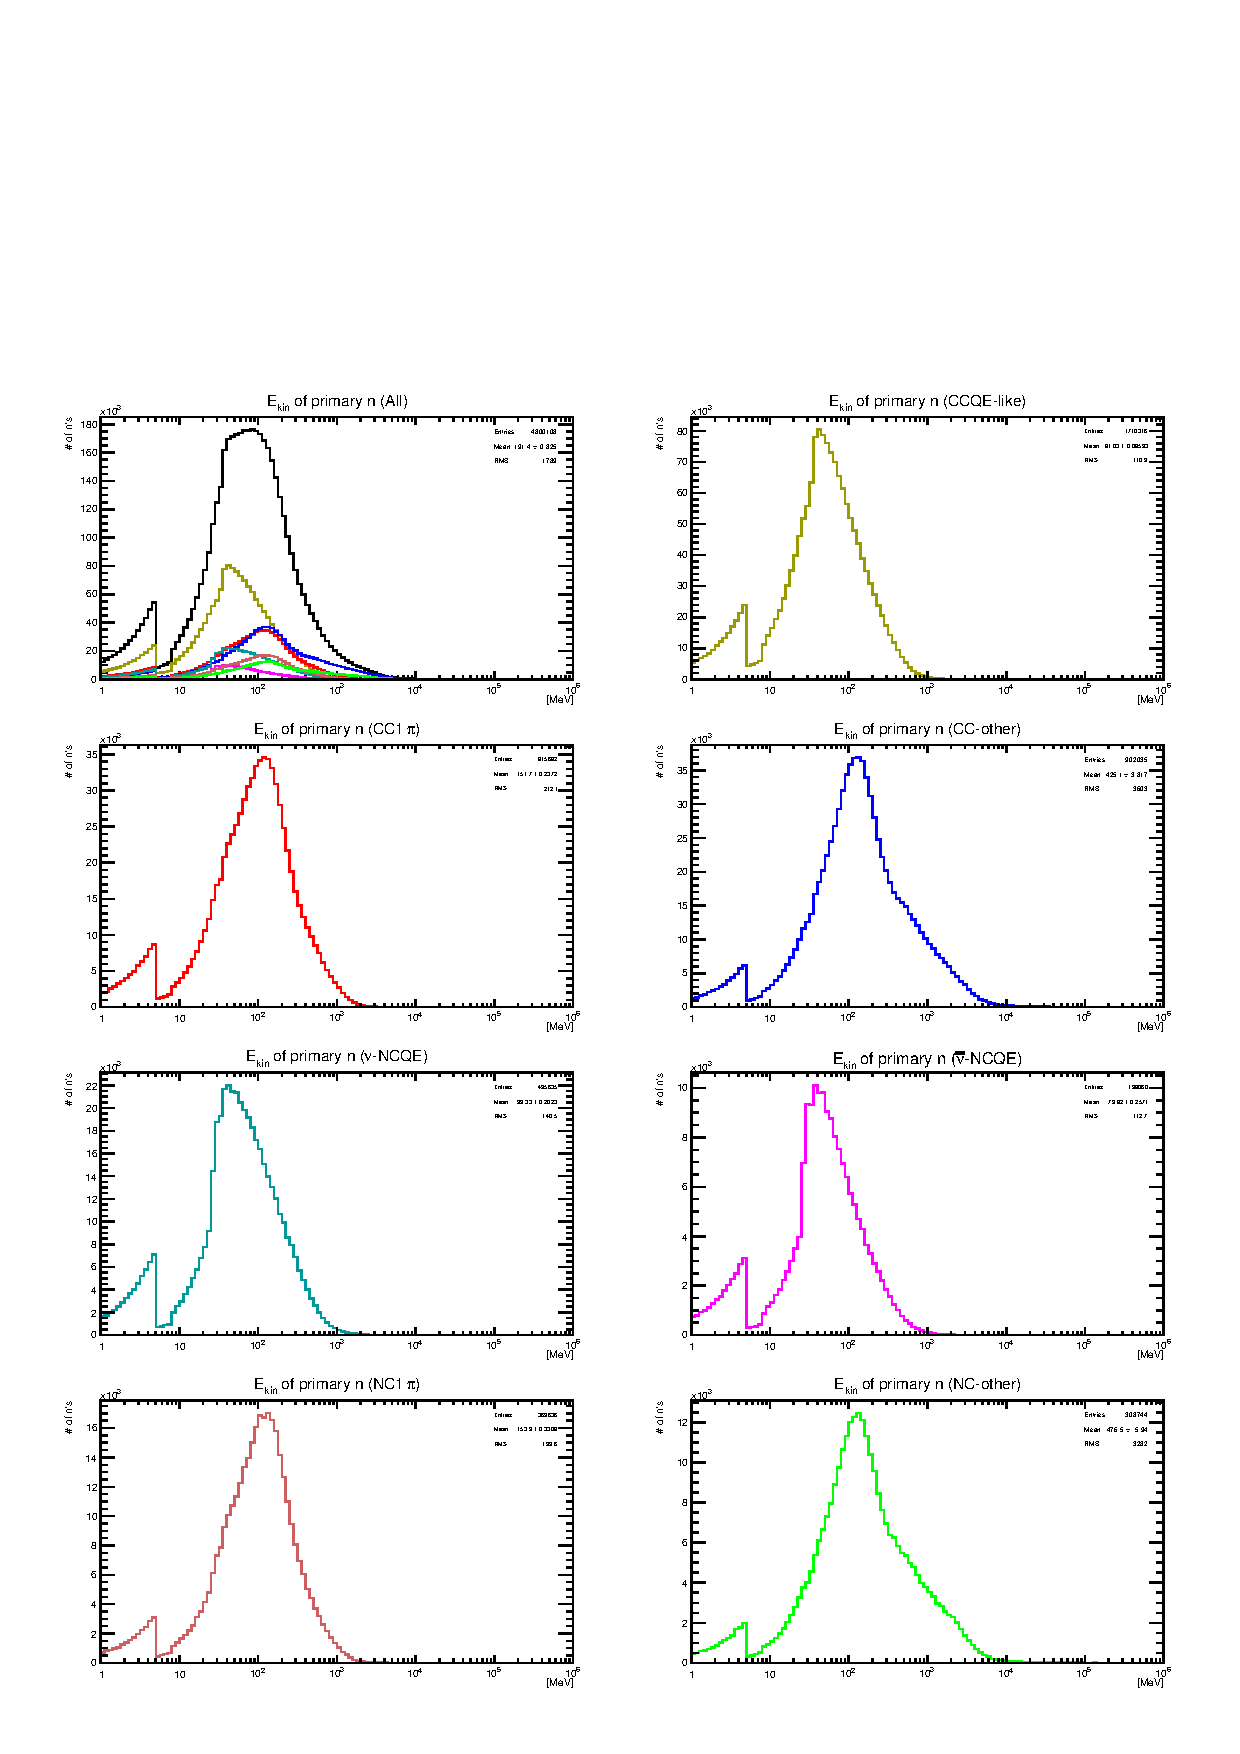
\includegraphics[width=16cm]{PDF/NEUT/s1_2_official/neutron/LogEnePri}
	\caption[Kinetic energy of neutrons generated by neutrino-nucleus interactions]{
	Kinetic energy of neutrons generated by neutrino-nucleus interactions.
	These figures were made using 500 years' worth of atmospheric neutrino events.
	}\label{neutronLogEnePri}
\end{figure}

\begin{figure}[h]
	\centering
	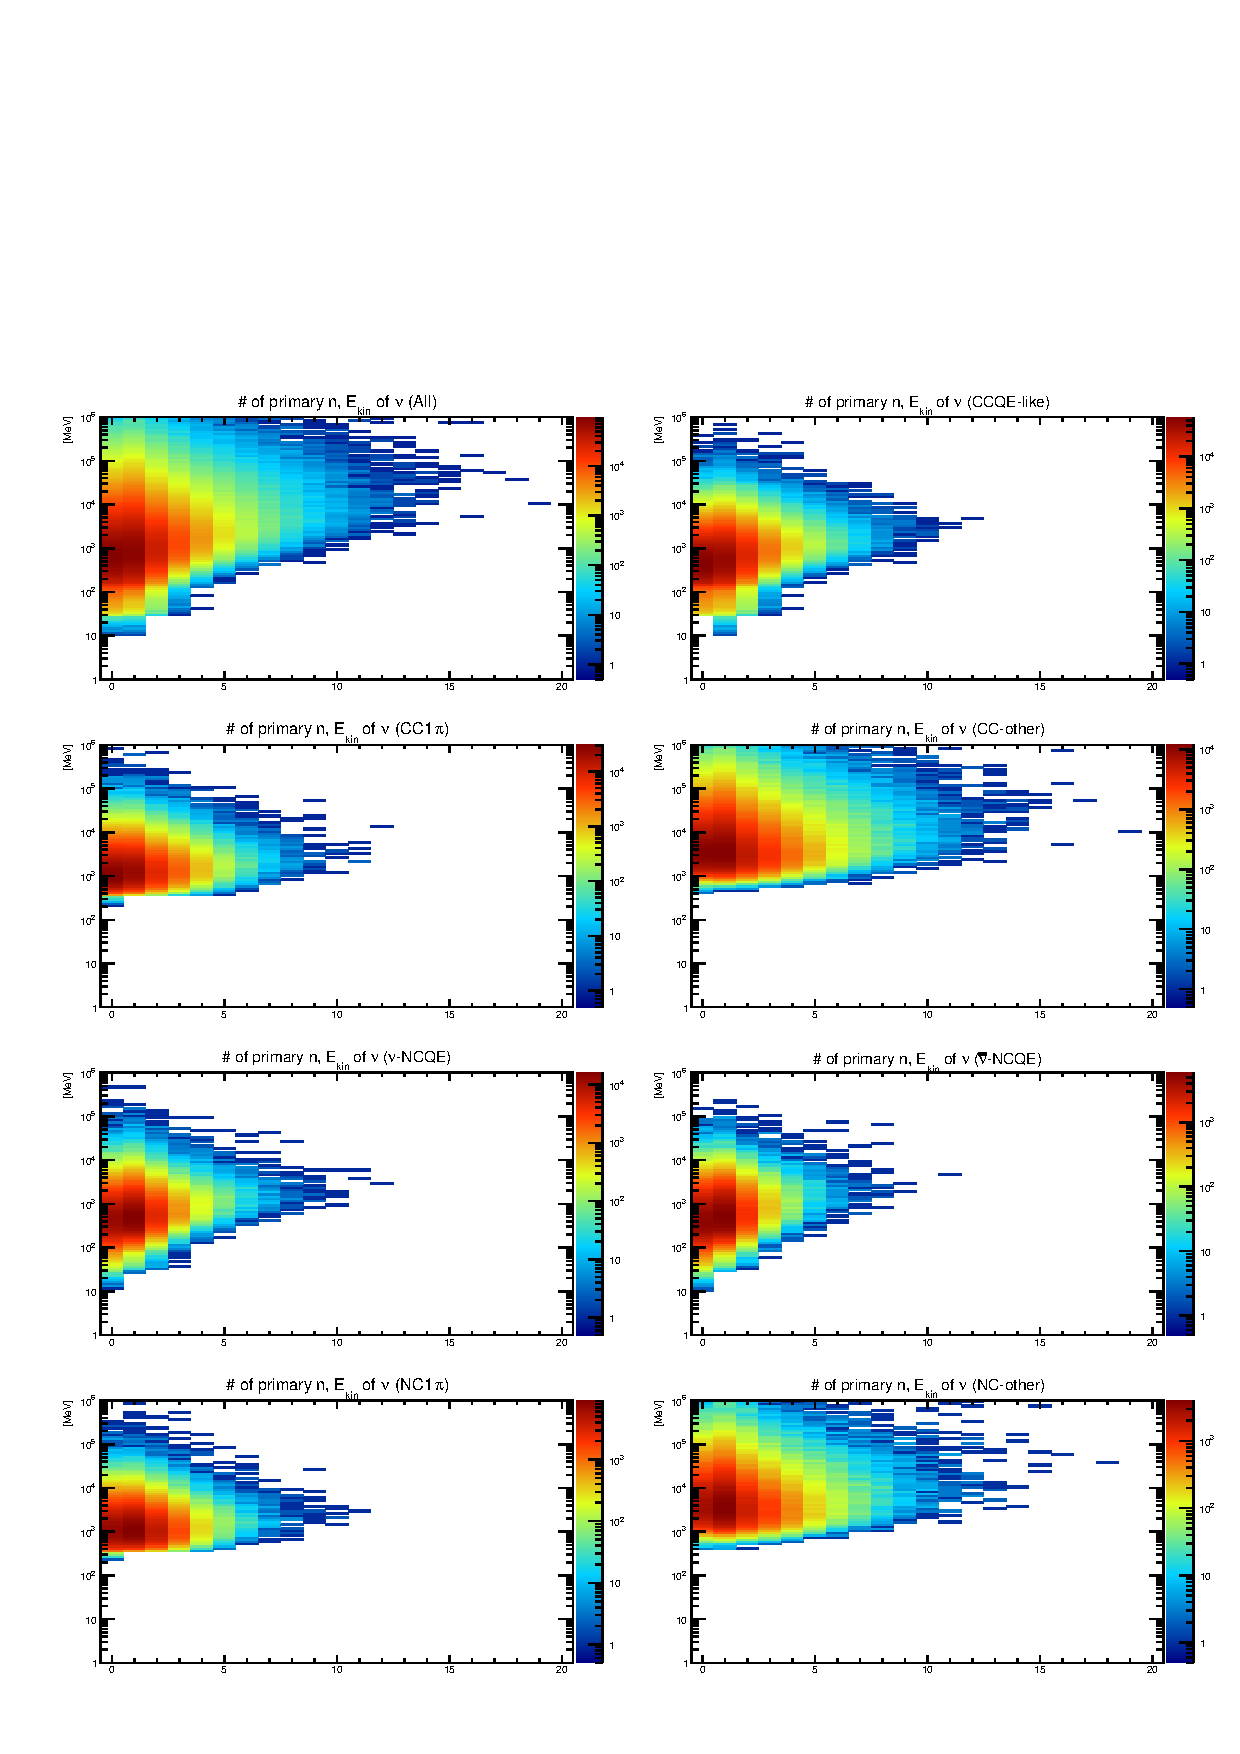
\includegraphics[width=16cm]{PDF/NEUT/s1_2_official/neutron_2D/Logz_NumPri_LogEneNeu}
	\caption[2D distribution of the number of neutrons generated by neutrino-nucleus interactions and energy of atmospheric neutrinos that induced neutrino-nucleus interactions]{
	2D distribution of the number of neutrons generated by neutrino-nucleus interactions (the horisontal axis) and energy of atmospheric neutrinos that induced neutrino-nucleus interactions (the vertical axis).
	These figures were made using 500 years' worth of atmospheric neutrino events.
	}\label{neutron_2DLogz_NumPri_LogEneNeu}
\end{figure}





\clearpage
\subsection{Event selection}\label{App_Selection}
\vs\hs
Other distributions related to Section~\ref{Section_Selection} are summarized here.

\begin{figure}[H]
	\centering
	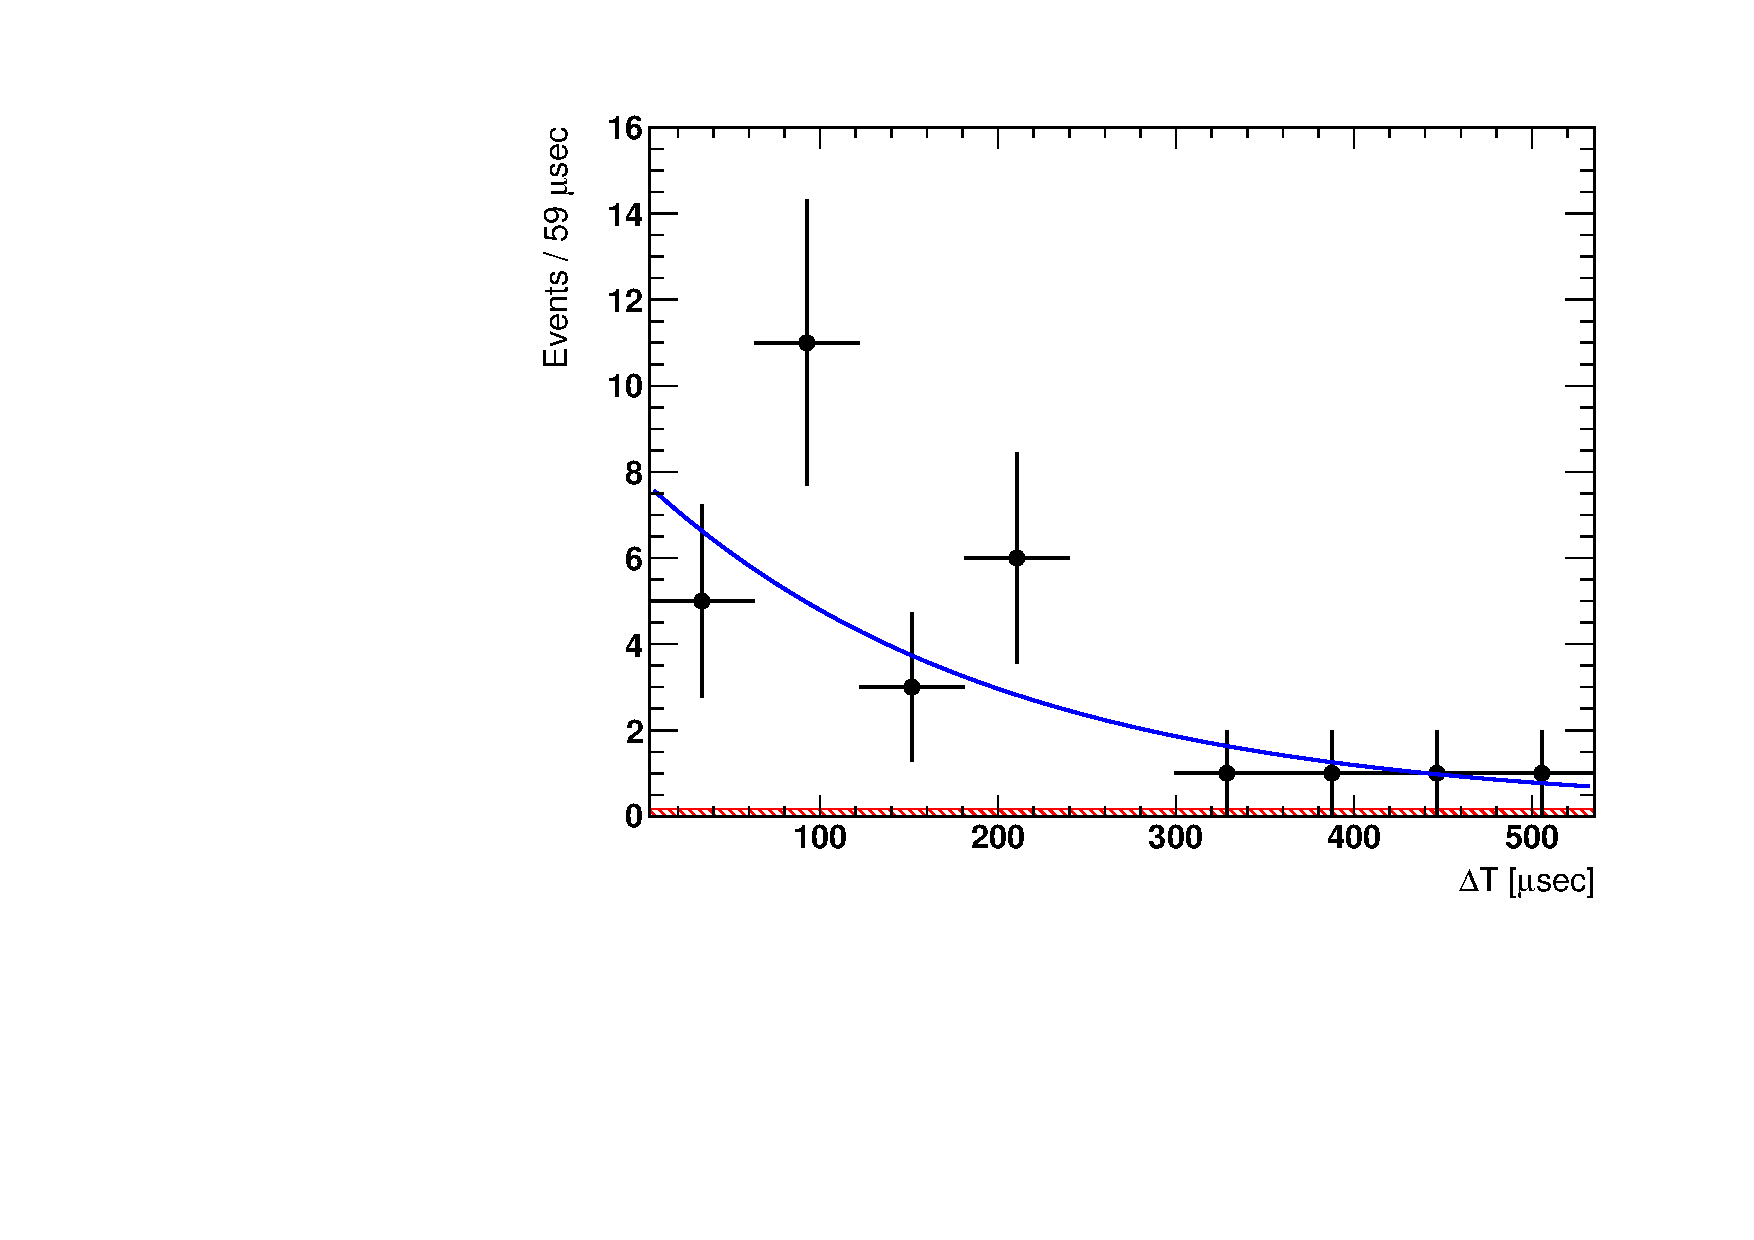
\includegraphics[width=10cm]{PDF/Figure03/Figure03}
	\caption[Timing of delayed signals]{
	Timing of delayed signals.
	Black plots show the data that $N_{\rm delayed} = 1$.
	Red area shows the accidental coincidence events.
	Blue line shows the fitted exponential distribution ($p_{0}\exp(-x/p_{1}) + p_{2}$).
	In this distribution, $p_{0} = 7.646 \pm 2.470$ and $p_{1} = 198.5 \pm 62.1$~[$\mu$s].
	The constant term ($p_{2}$) was fixed at the number of accidental coincidence events per bin ($=1.5524/9$) during the fitting.
	}\label{Figure03}
\end{figure}

\begin{figure}[H]
	\centering
	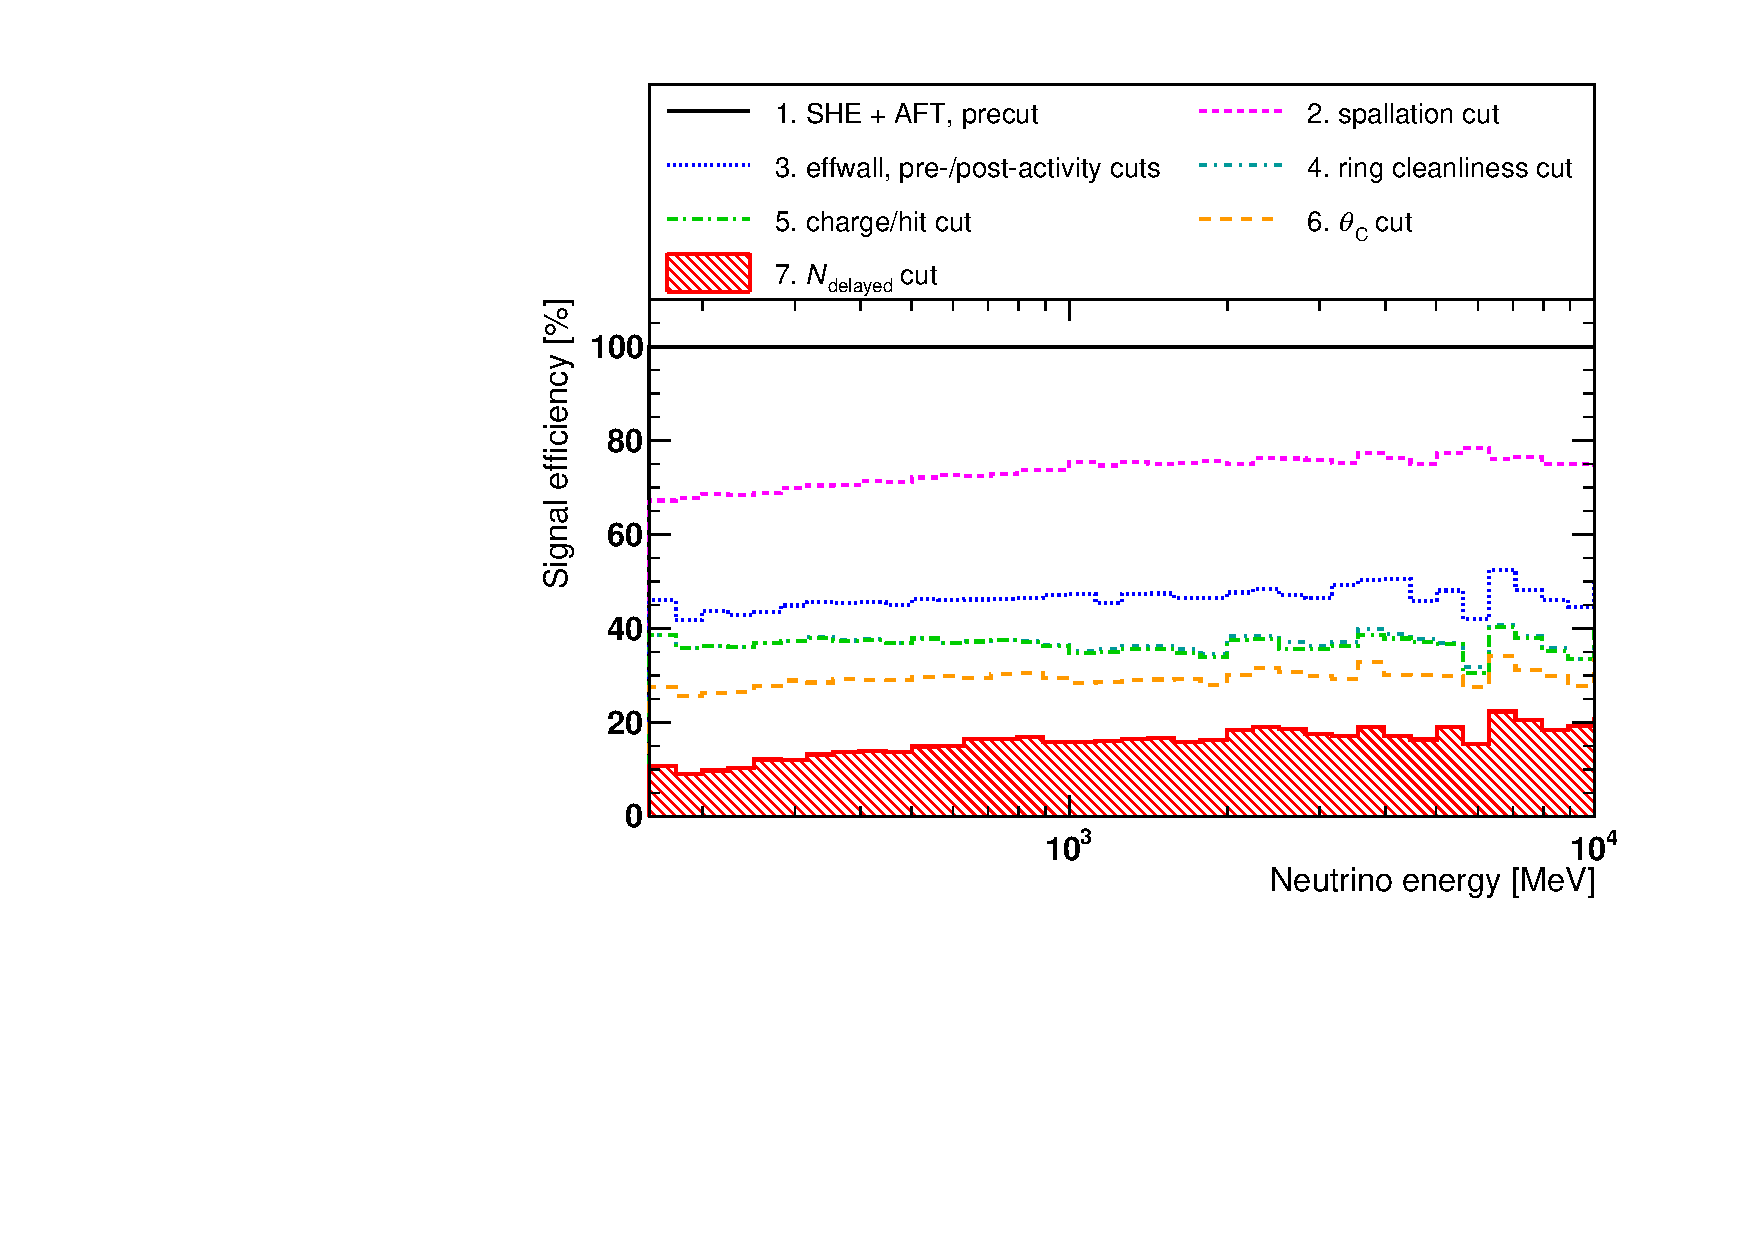
\includegraphics[width=10cm]{PDF/Figure06/FTFP_BERT_HP/Figure06}
	\caption[NCQE cumulative signal efficiencies as a function of neutrino energy]{
	NCQE cumulative signal efficiencies as a function of neutrino energy.
	Event reductions are performed in the order shown in the legend, and before the reduction for spallation events is taken as 100\%.
	}\label{BERT_Figure06}
\end{figure}

\begin{figure}[h]
	\centering
	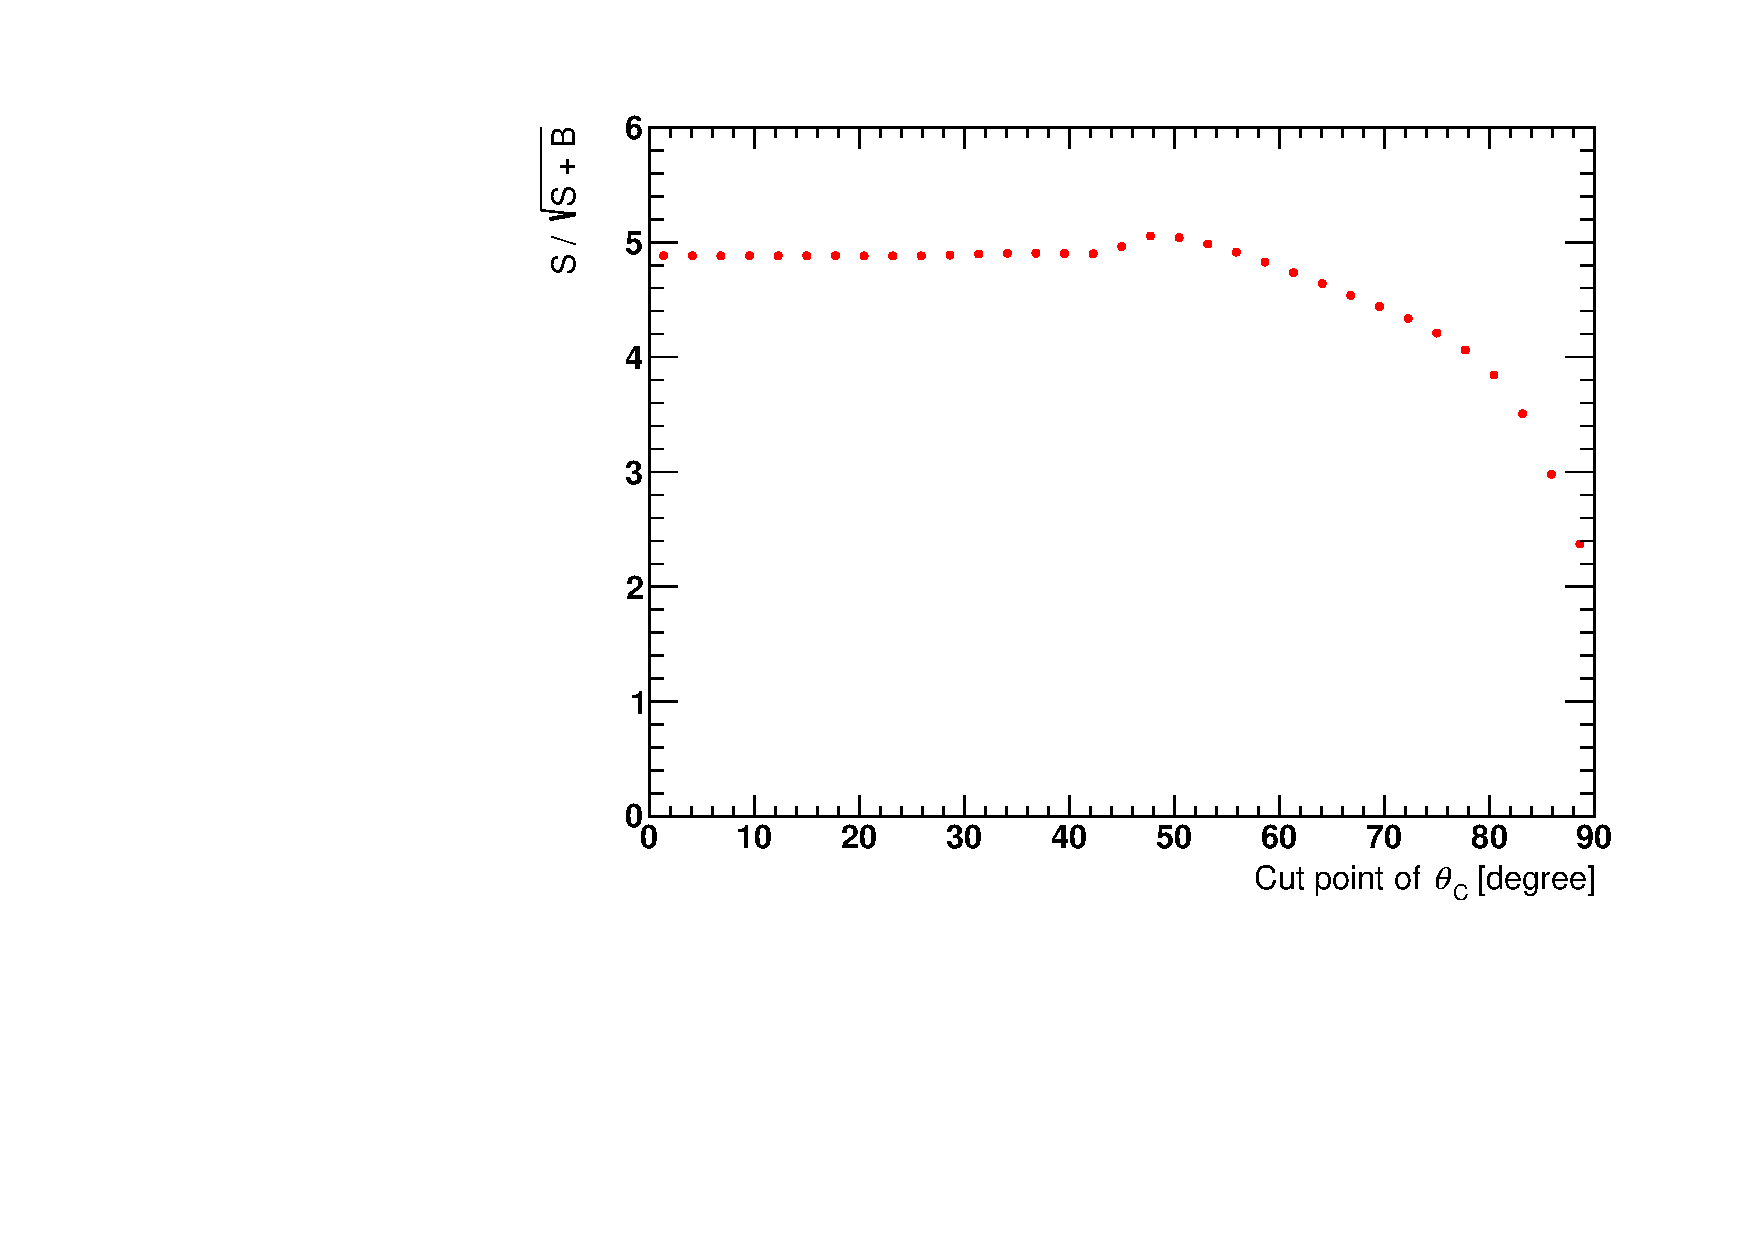
\includegraphics[width=10cm]{PDF/230526_SB/Figure_230526_SB_woNCnonQE}
	\caption[Singal-to-background ratio]{
	Singal-to-background ratio.
	Horizontal axis shows the $\theta_{\rm C}$ cut point.
	Vertical axis shows the singal-to-background ratio $S/\sqrt{S + B}$, where $S$ is the expected number of NCQE events and $B$ is the expected number of events, including CC, spallation, reactor neutrino, and accidental coincidence.
	}\label{Figure_230526_SB_woNCnonQE}
\end{figure}

\begin{figure}[h]
	\centering
	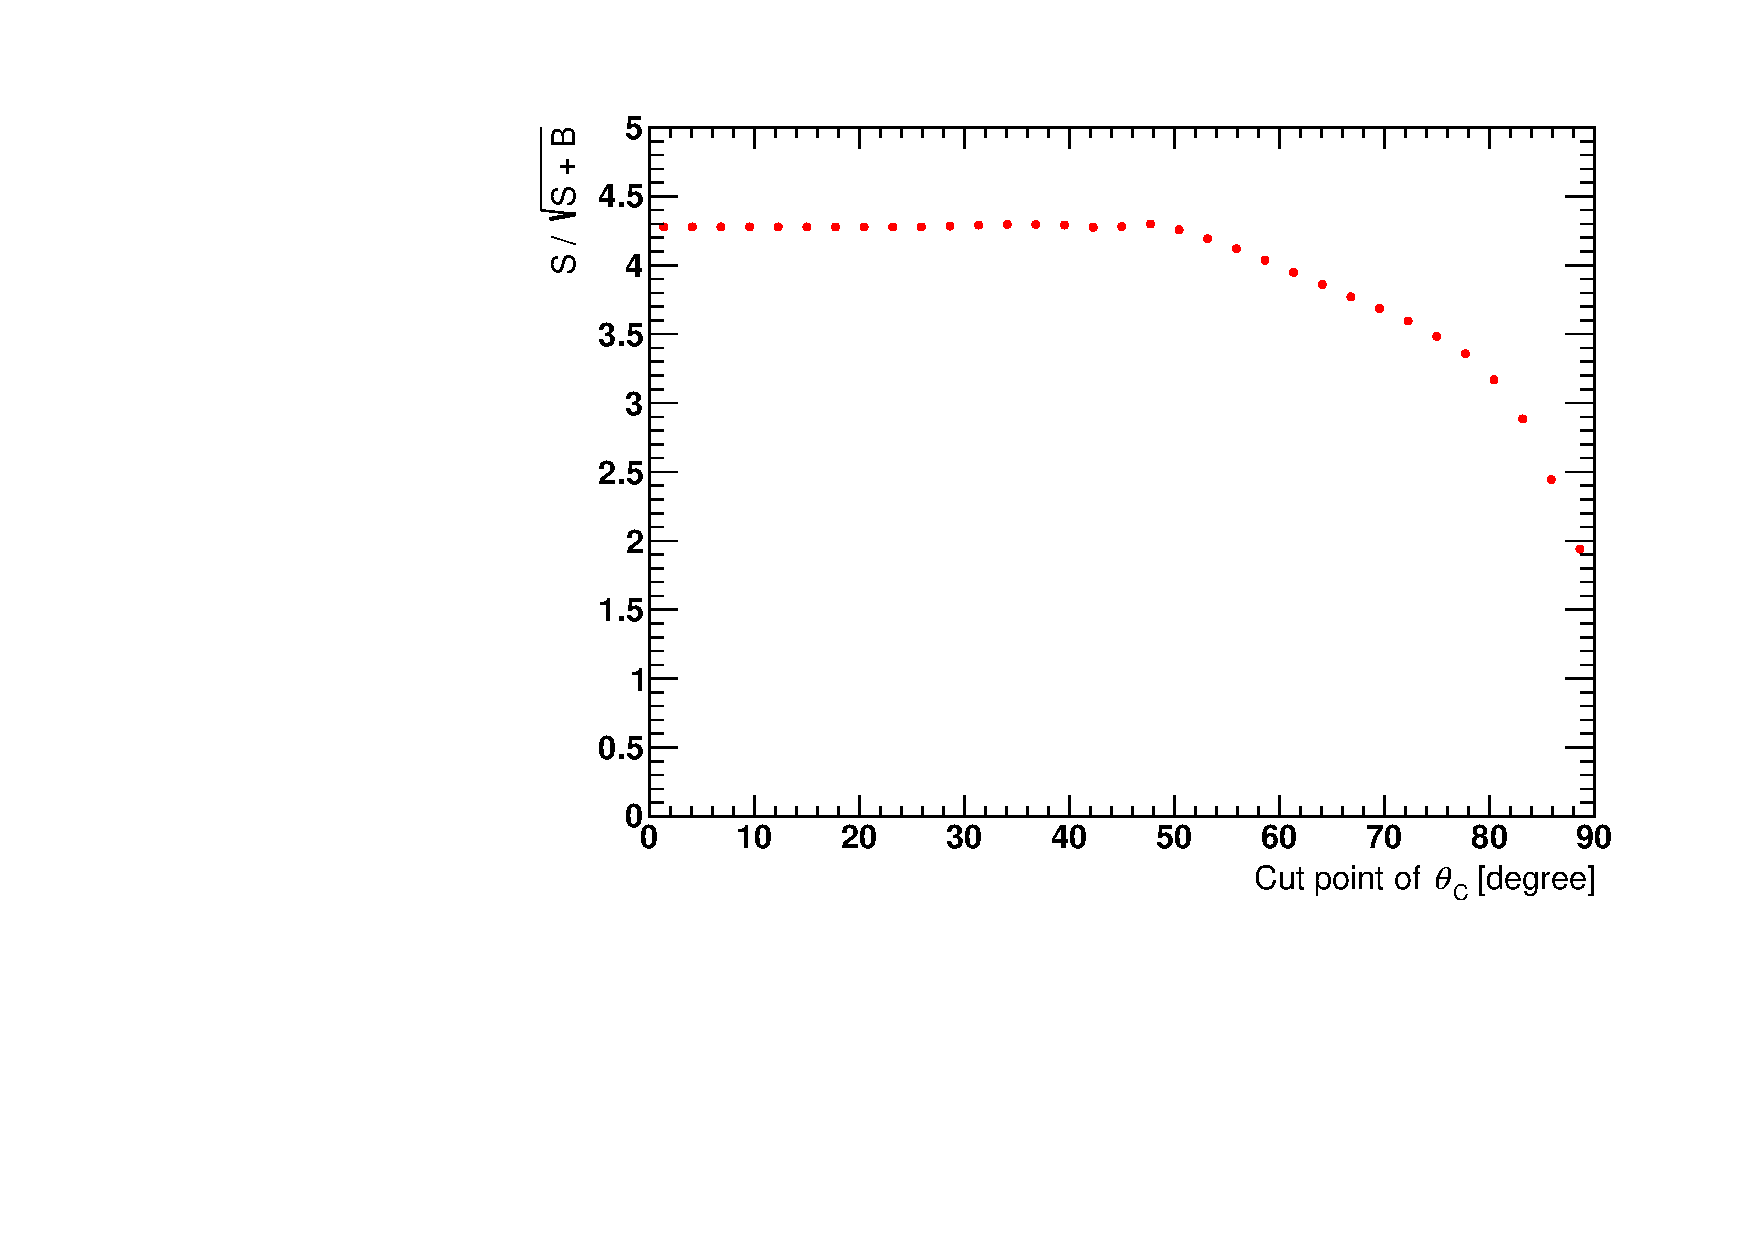
\includegraphics[width=10cm]{PDF/230526_SB/Figure_230526_SB}
	\caption[Singal-to-background ratio]{
	Singal-to-background ratio.
	Horizontal axis shows the $\theta_{\rm C}$ cut point.
	Vertical axis shows the singal-to-background ratio $S/\sqrt{S + B}$, where $S$ is the expected number of NCQE events and $B$ is the expected number of events, including NC non-QE, CC, spallation, reactor neutrino, and accidental coincidence.
	}\label{Figure_230526_SB}
\end{figure}

\begin{figure}[h]
	\centering
	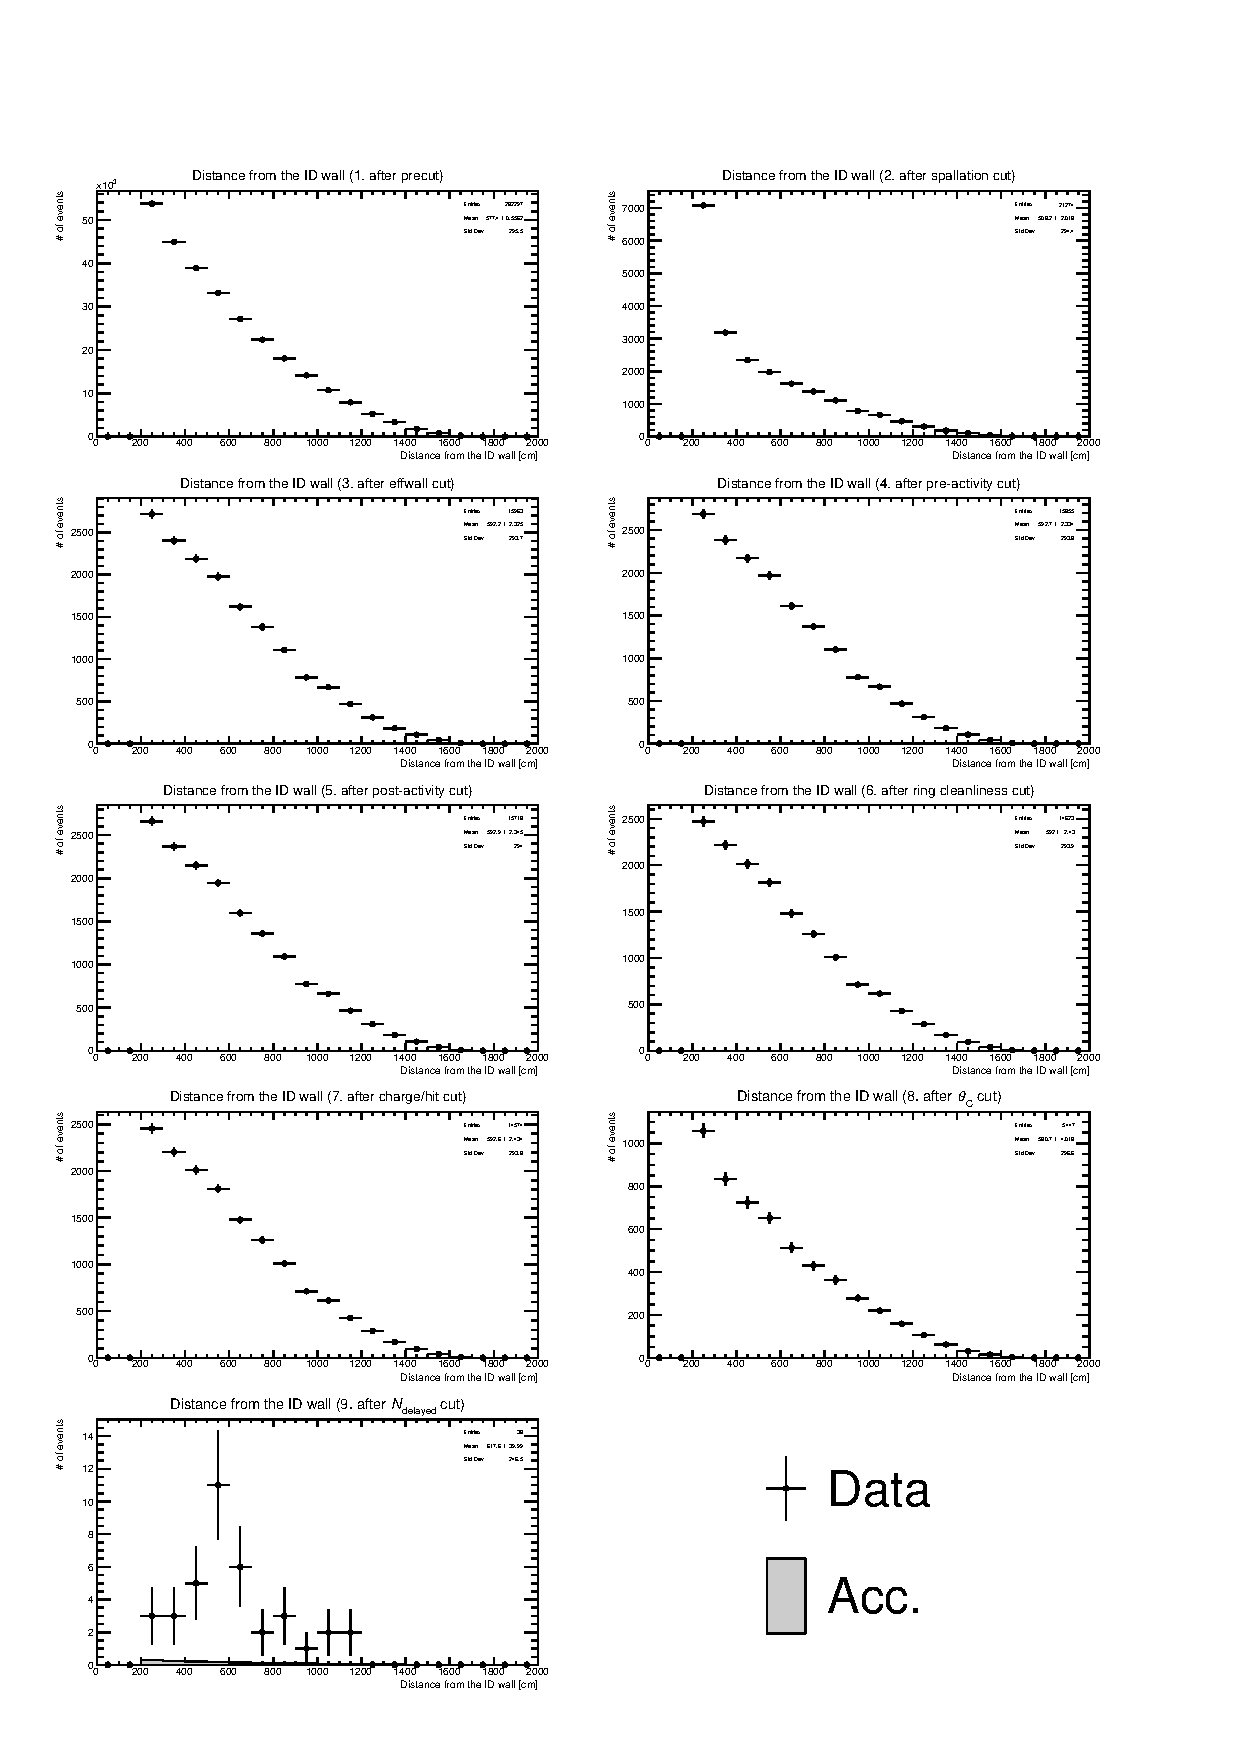
\includegraphics[width=15cm]{PDF/Dist_Data/Che_50deg_tag_ge1/dwall}
	\caption[Distance from the ID wall for the data and accidental coincidence events]{
	Distance form the ID wall for the data and accidental coincidence events.
	Event reductions are performed in the order shown in the title.
	}\label{Data_dwall}
\end{figure}

\begin{figure}[h]
	\centering
	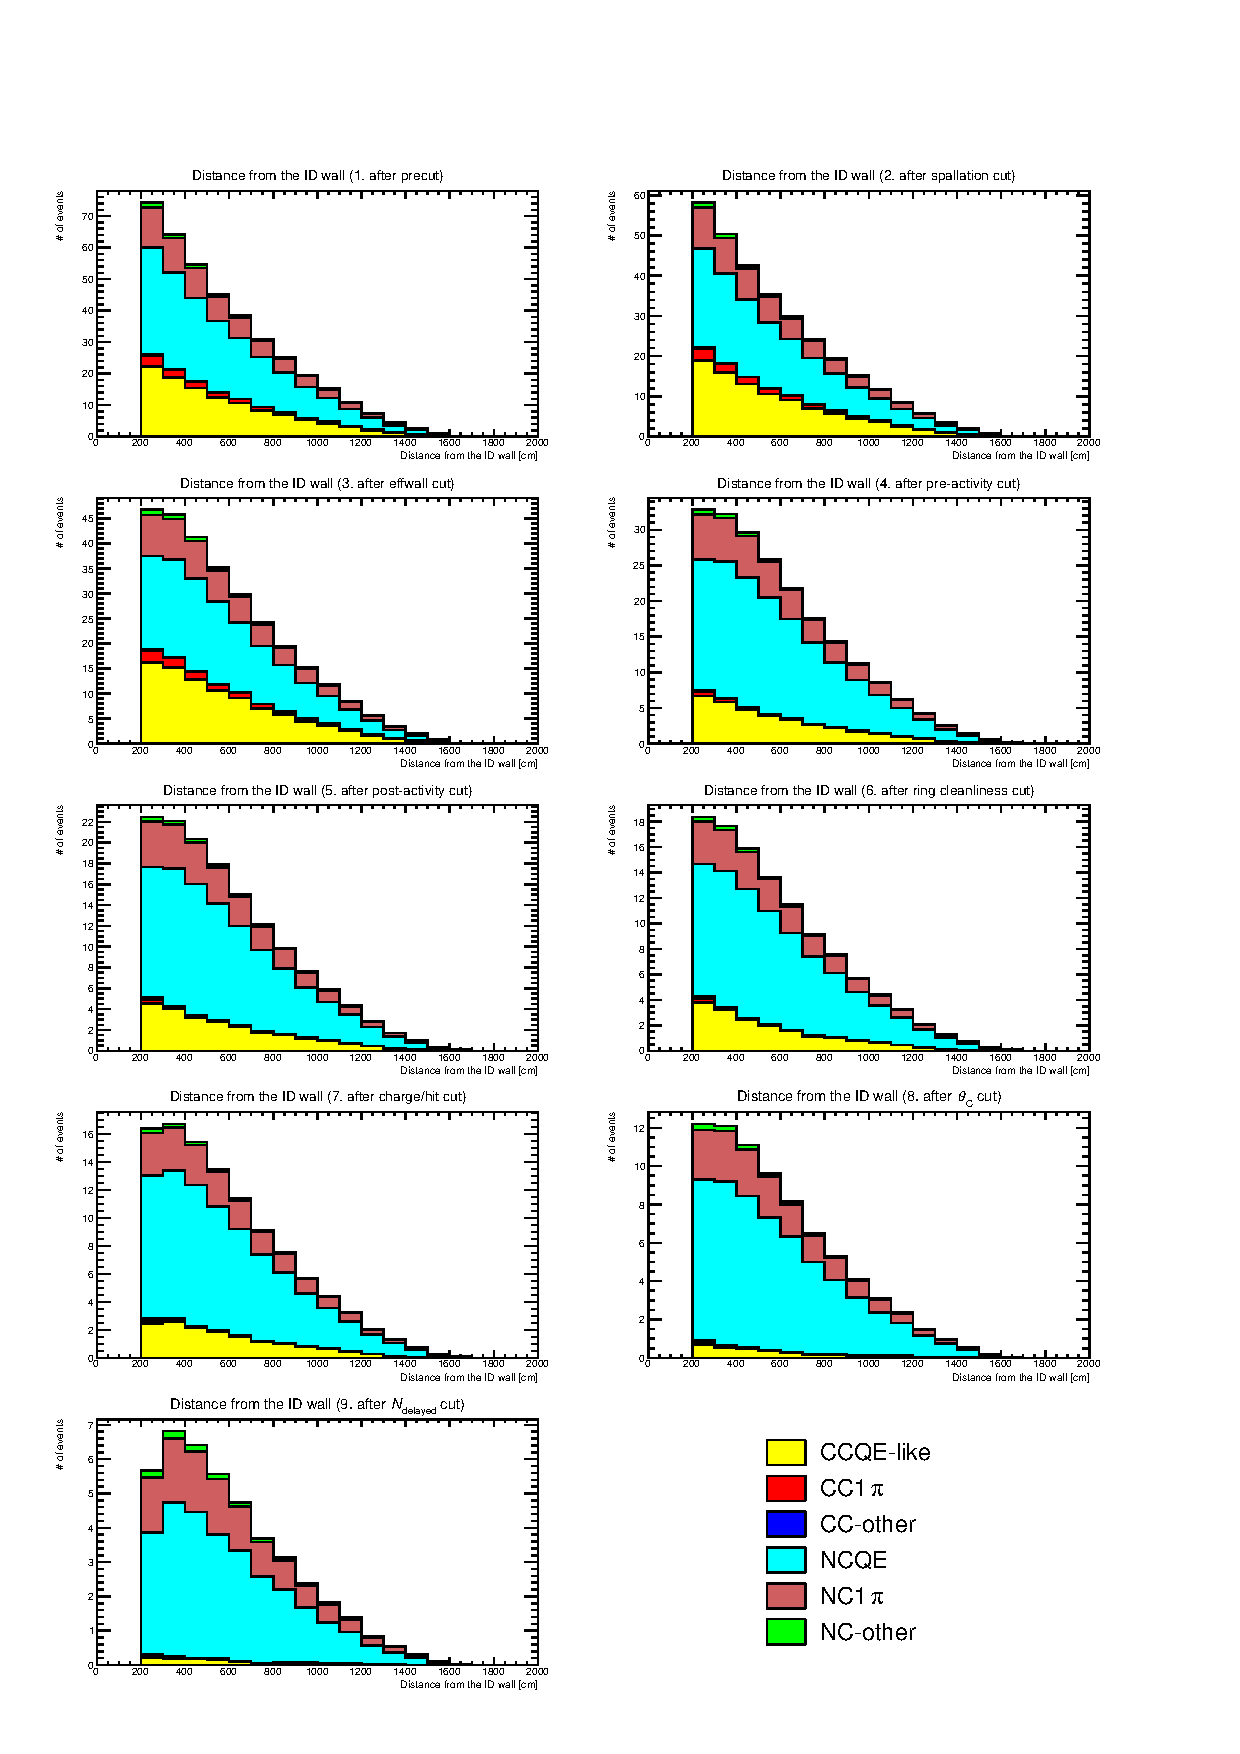
\includegraphics[width=15cm]{PDF/Dist_ATM/Che_50deg_tag_ge1/All/dwall}
	\caption[Distance from the ID wall for atmospheric neutrino events]{
	Distance form the ID wall for atmospheric neutrino events.
	Event reductions are performed in the order shown in the title.
	}\label{ATM_dwall}
\end{figure}

\begin{figure}[h]
	\centering
	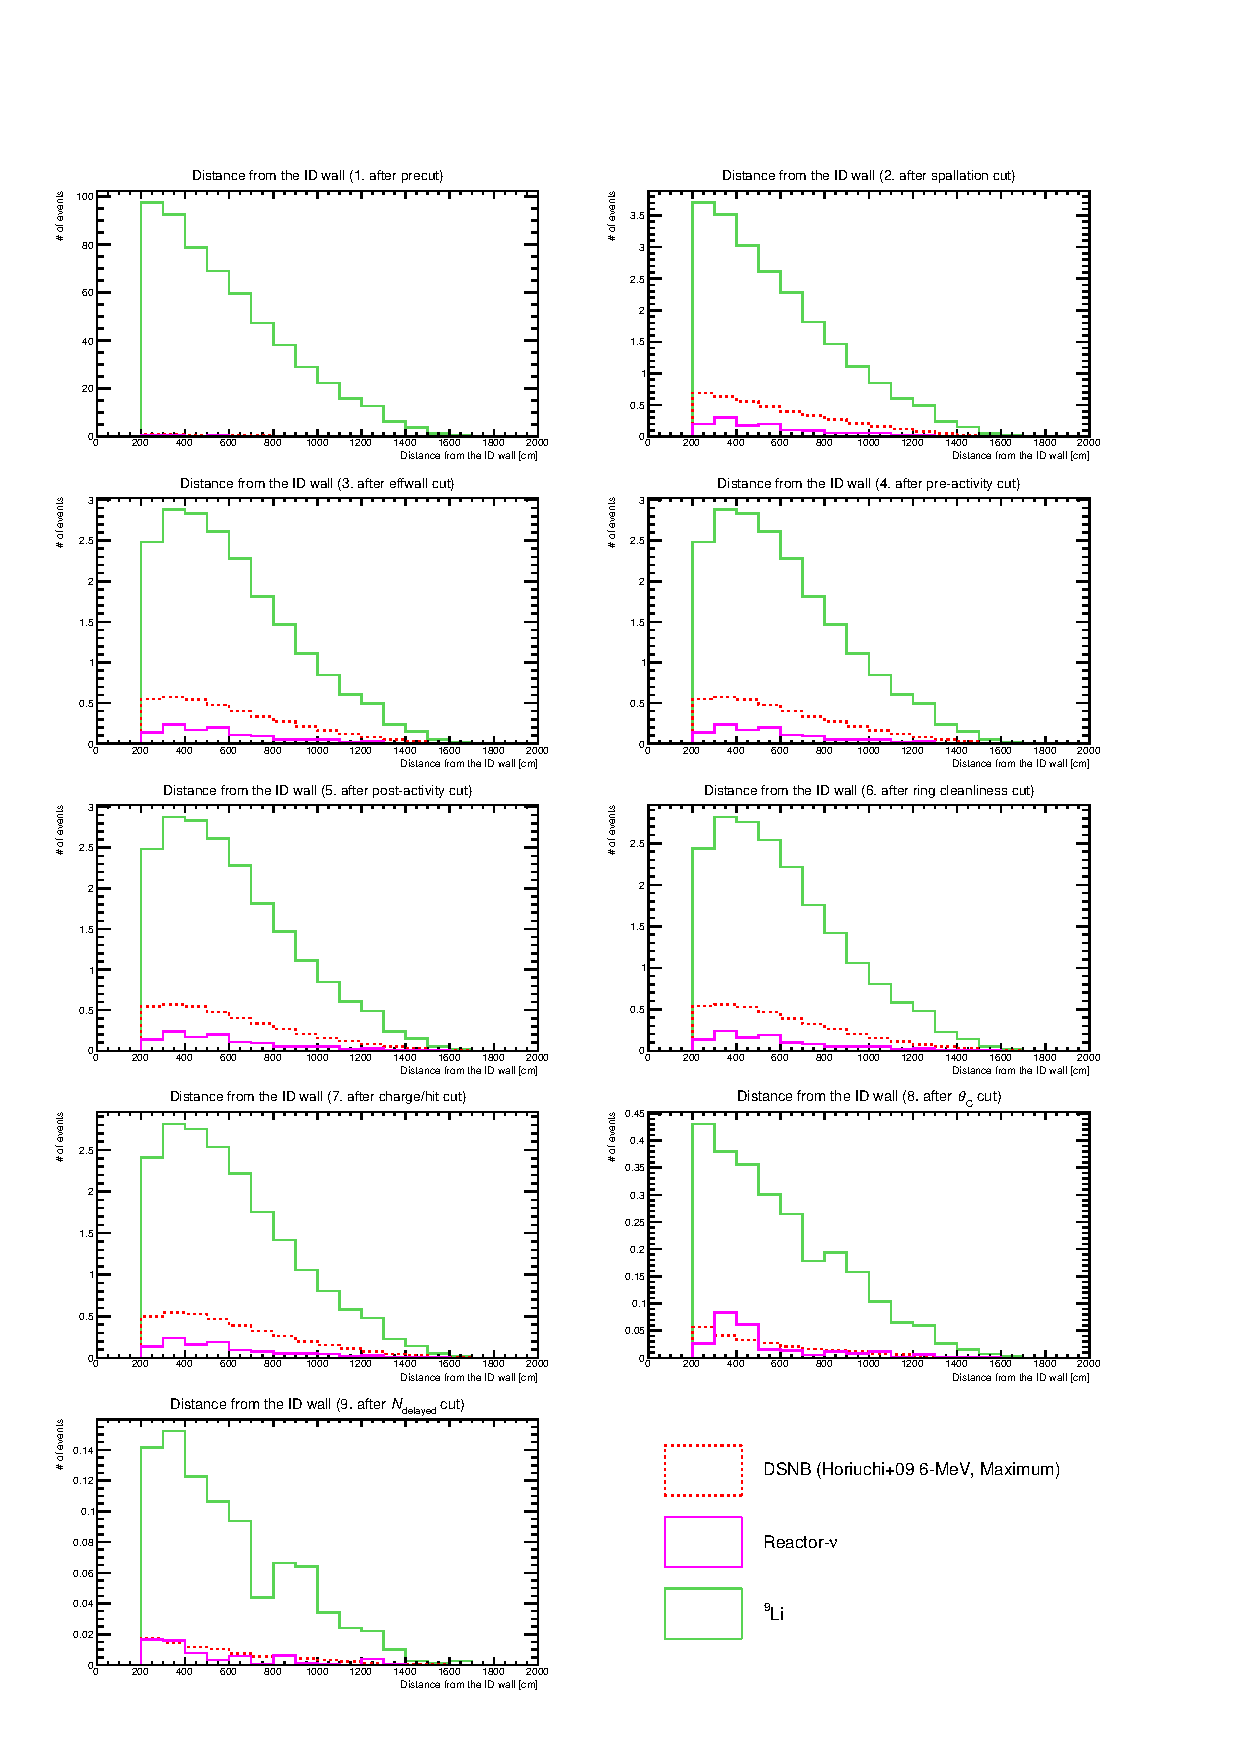
\includegraphics[width=15cm]{PDF/Dist_Nuebar/Che_50deg_tag_ge1/dwall}
	\caption[Distance from the ID wall for spallation, reactor neutrino, and DSNB events]{
	Distance form the ID wall for spallation, reactor neutrino, and DSNB events.
	Event reductions are performed in the order shown in the title.
	}\label{Nuebar_dwall}
\end{figure}

\begin{figure}[h]
	\centering
	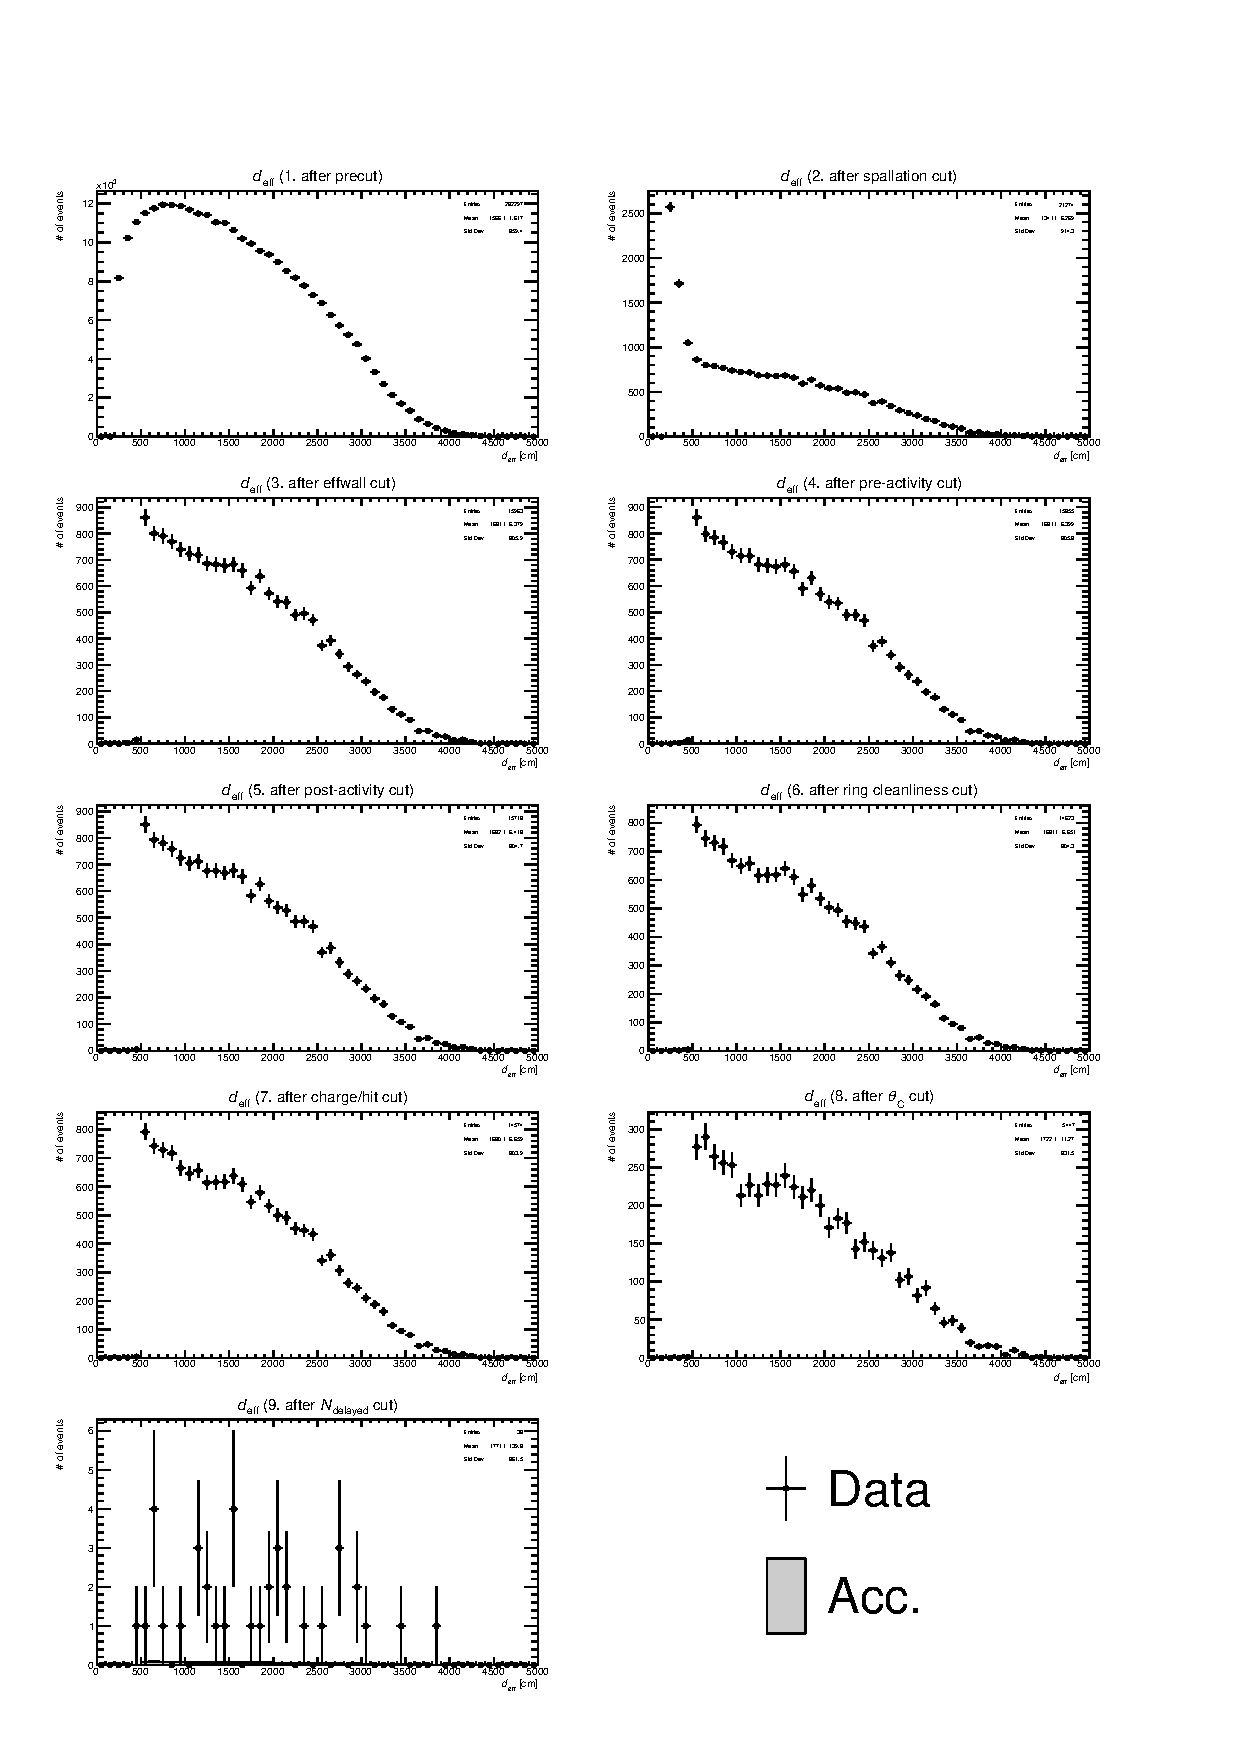
\includegraphics[width=15cm]{PDF/Dist_Data/Che_50deg_tag_ge1/effwall}
	\caption[$d_{\rm eff}$ for the data and accidental coincidence events]{
	$d_{\rm eff}$ for the data and accidental coincidence events.
	Event reductions are performed in the order shown in the title.
	}\label{Data_effwall}
\end{figure}

\begin{figure}[h]
	\centering
	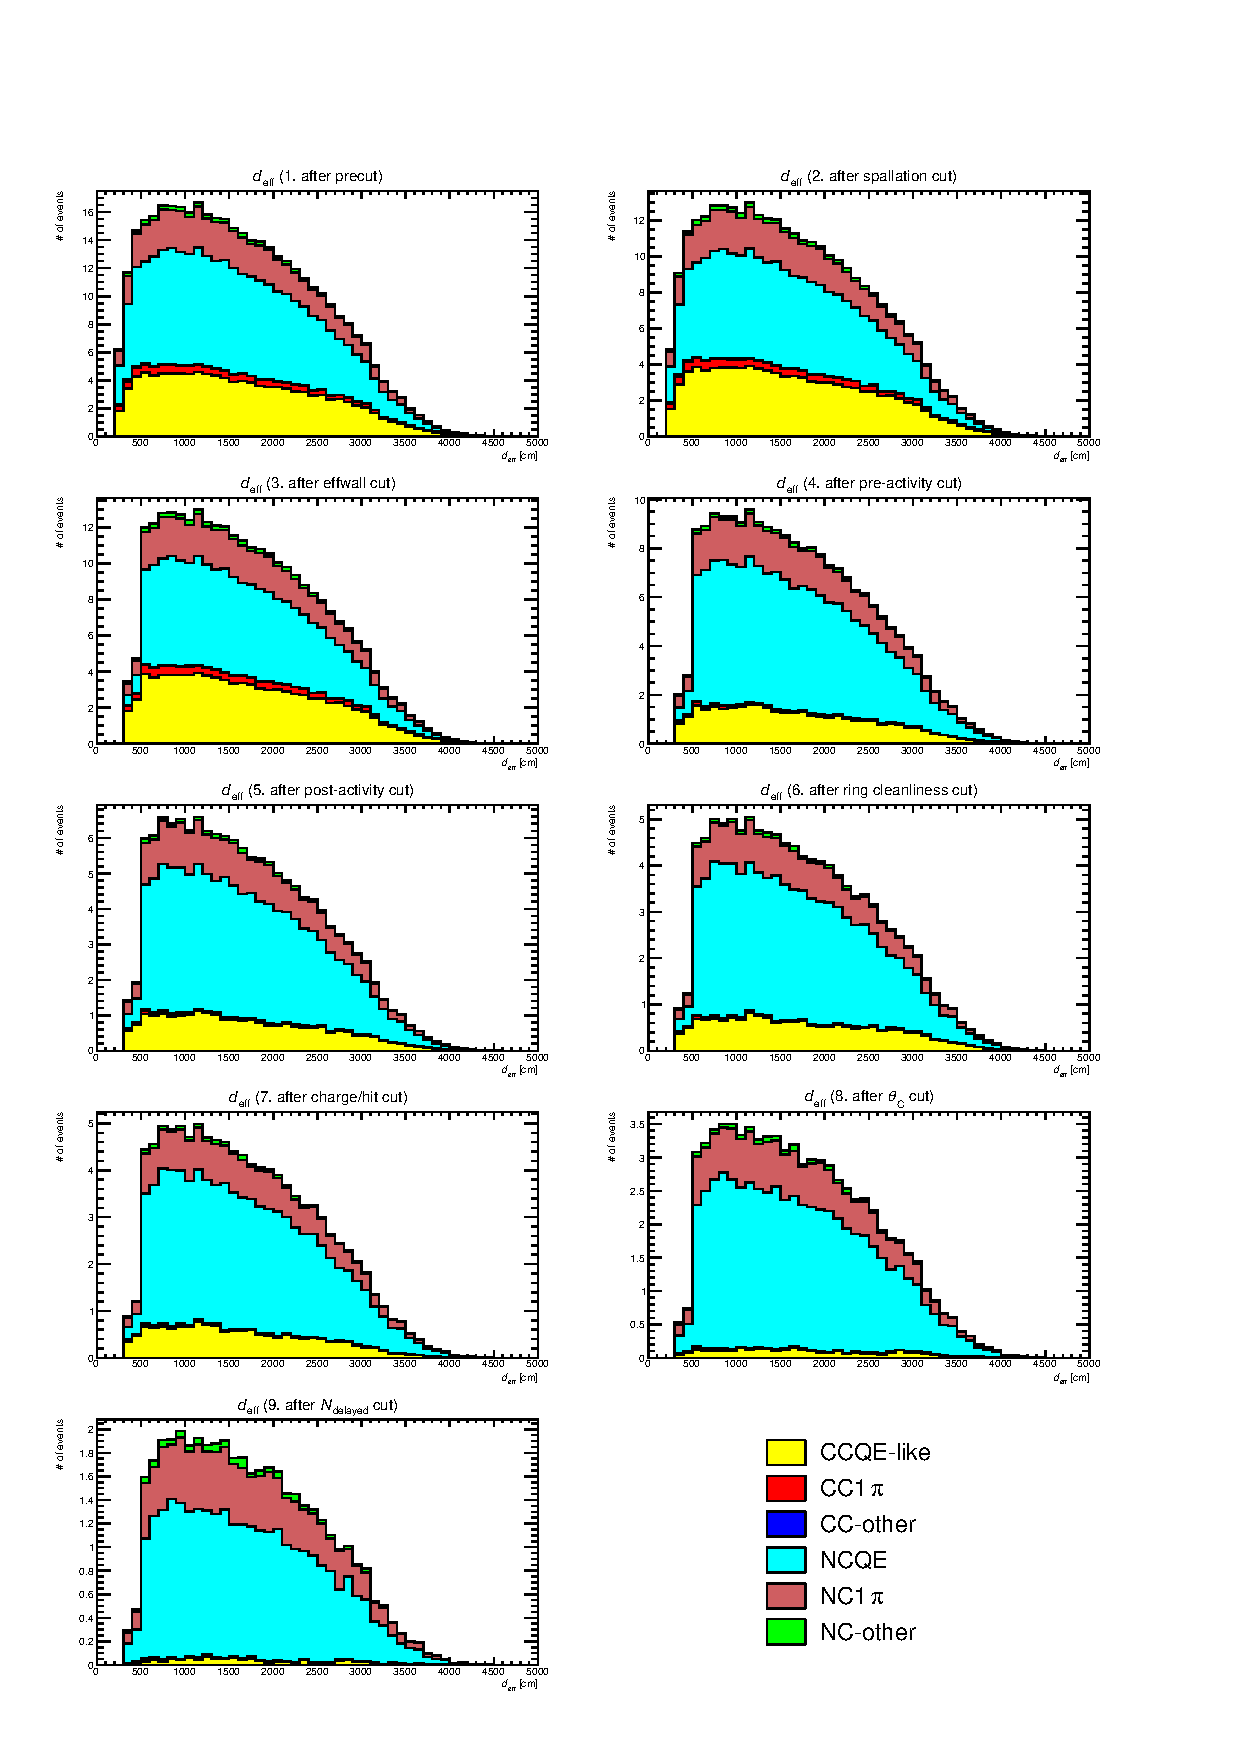
\includegraphics[width=15cm]{PDF/Dist_ATM/Che_50deg_tag_ge1/All/effwall}
	\caption[$d_{\rm eff}$ for atmospheric neutrino events]{
	$d_{\rm eff}$ for atmospheric neutrino events.
	Event reductions are performed in the order shown in the title.
	}\label{ATM_effwall}
\end{figure}

\begin{figure}[h]
	\centering
	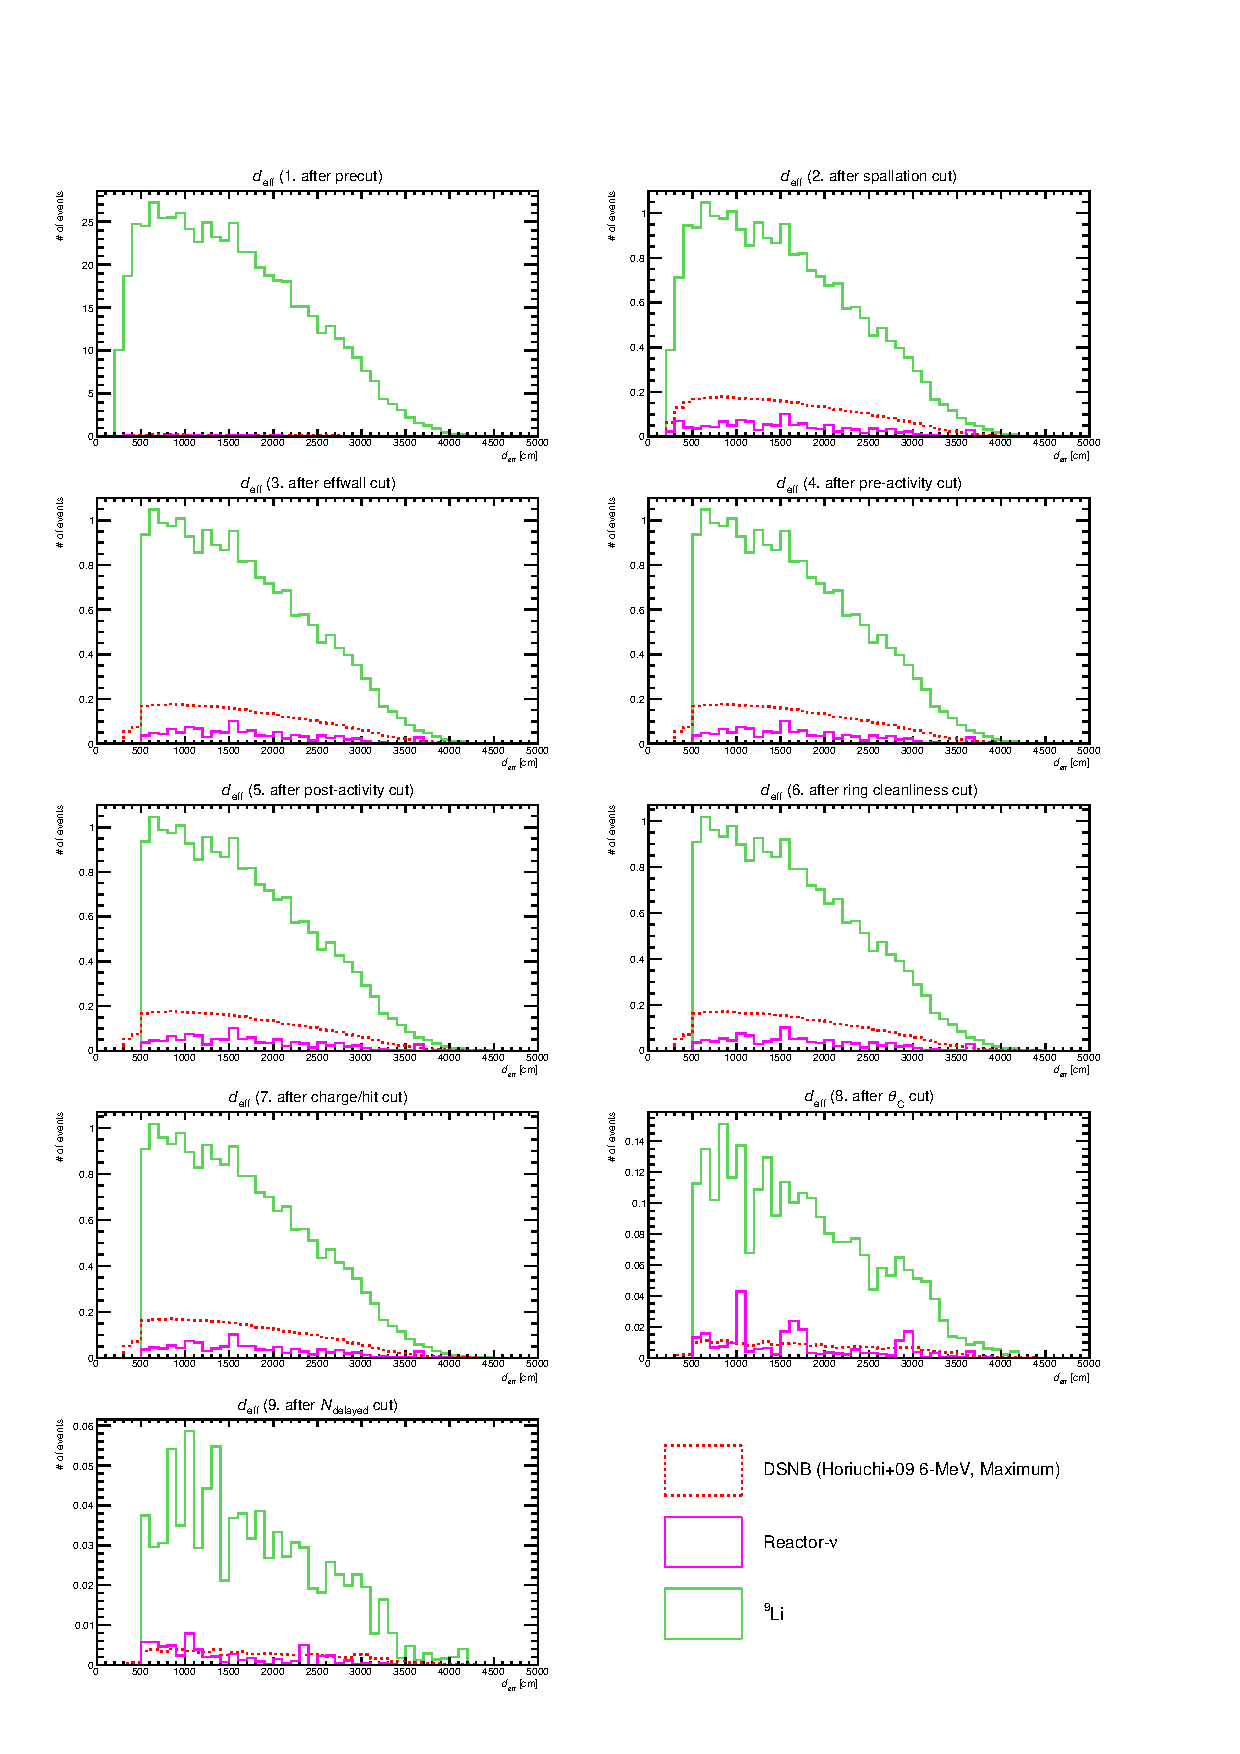
\includegraphics[width=15cm]{PDF/Dist_Nuebar/Che_50deg_tag_ge1/effwall}
	\caption[$d_{\rm eff}$ for spallation, reactor neutrino, and DSNB events]{
	$d_{\rm eff}$ for spallation, reactor neutrino, and DSNB events.
	Event reductions are performed in the order shown in the title.
	}\label{Nuebar_effwall}
\end{figure}

\begin{figure}[h]
	\centering
	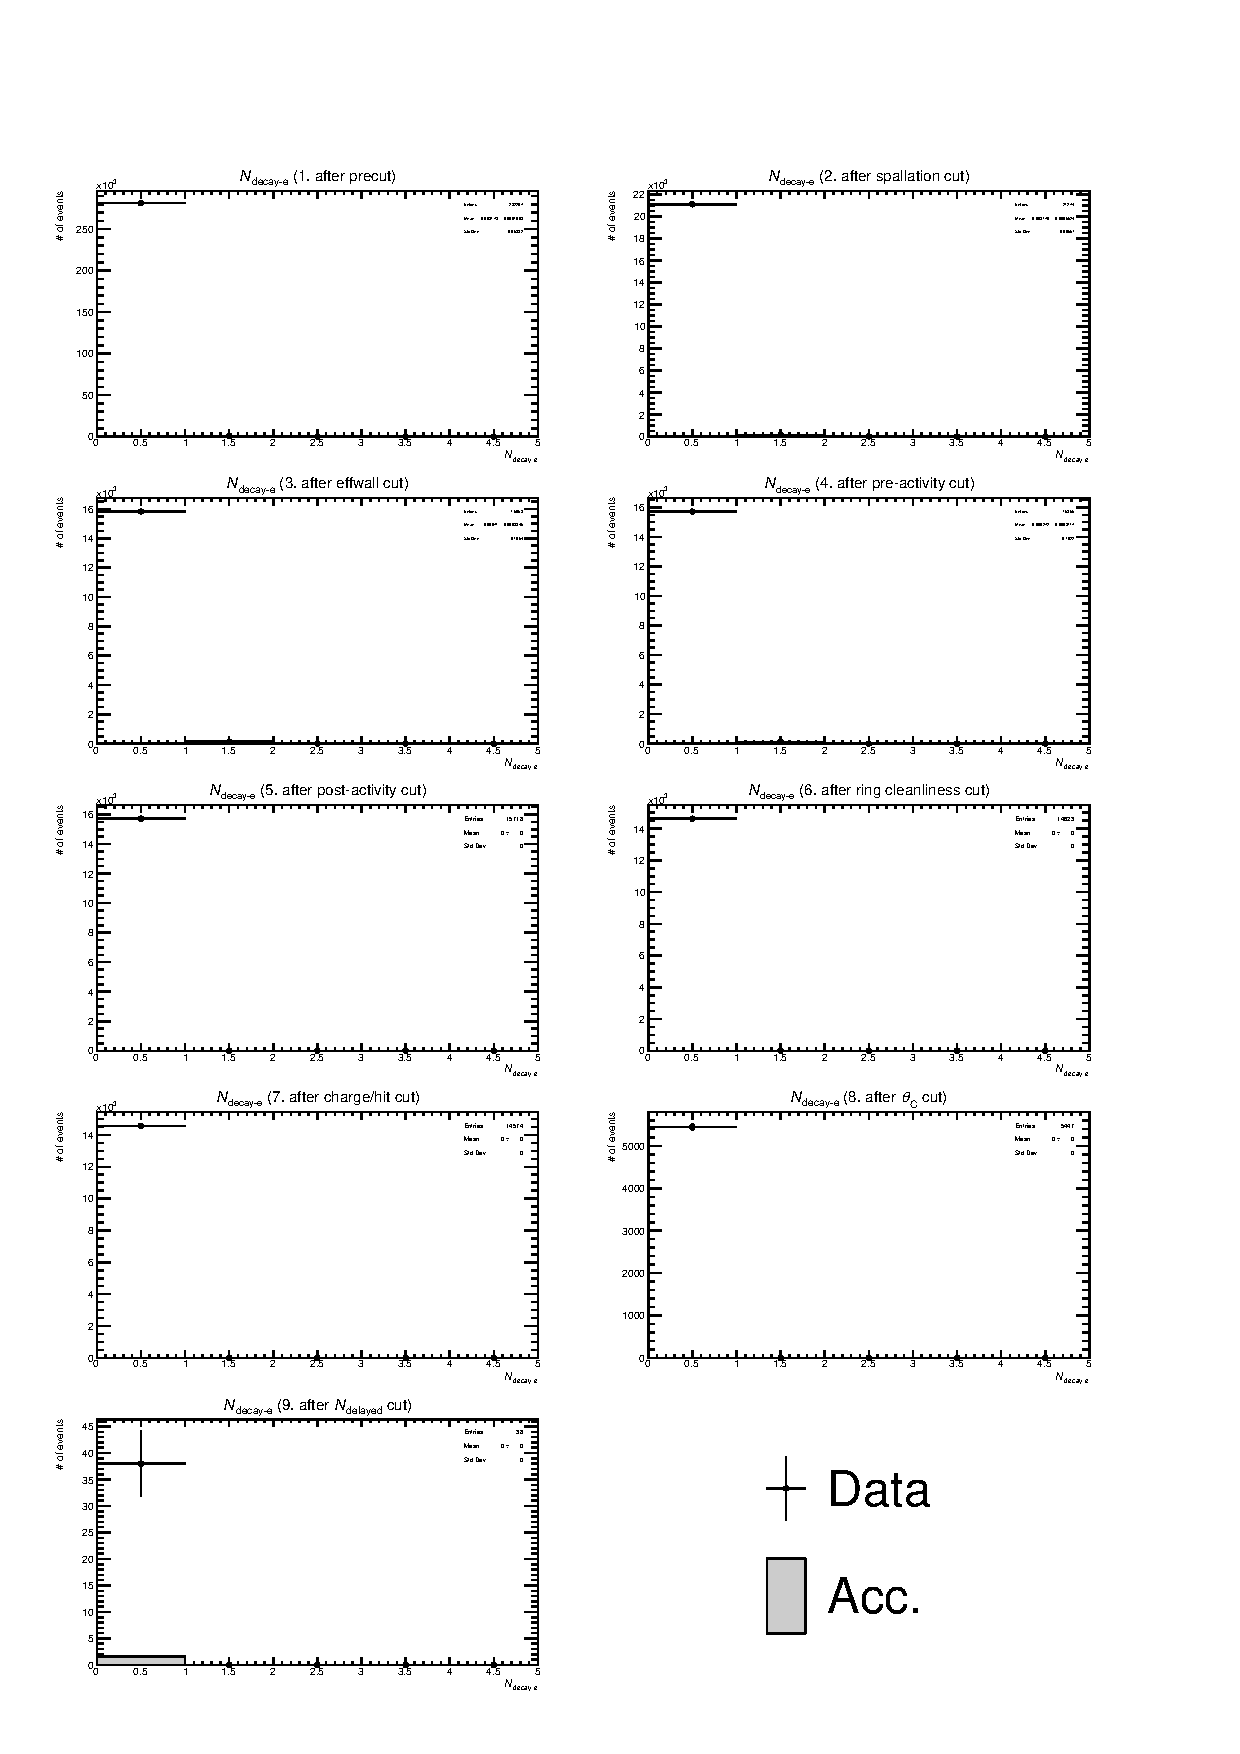
\includegraphics[width=15cm]{PDF/Dist_Data/Che_50deg_tag_ge1/nmue}
	\caption[$N_{\rm decay\mathchar`-e}$ for the data and accidental coincidence events]{
	$N_{\rm decay\mathchar`-e}$ for the data and accidental coincidence events.
	Event reductions are performed in the order shown in the title.
	}\label{Data_nmue}
\end{figure}

\begin{figure}[h]
	\centering
	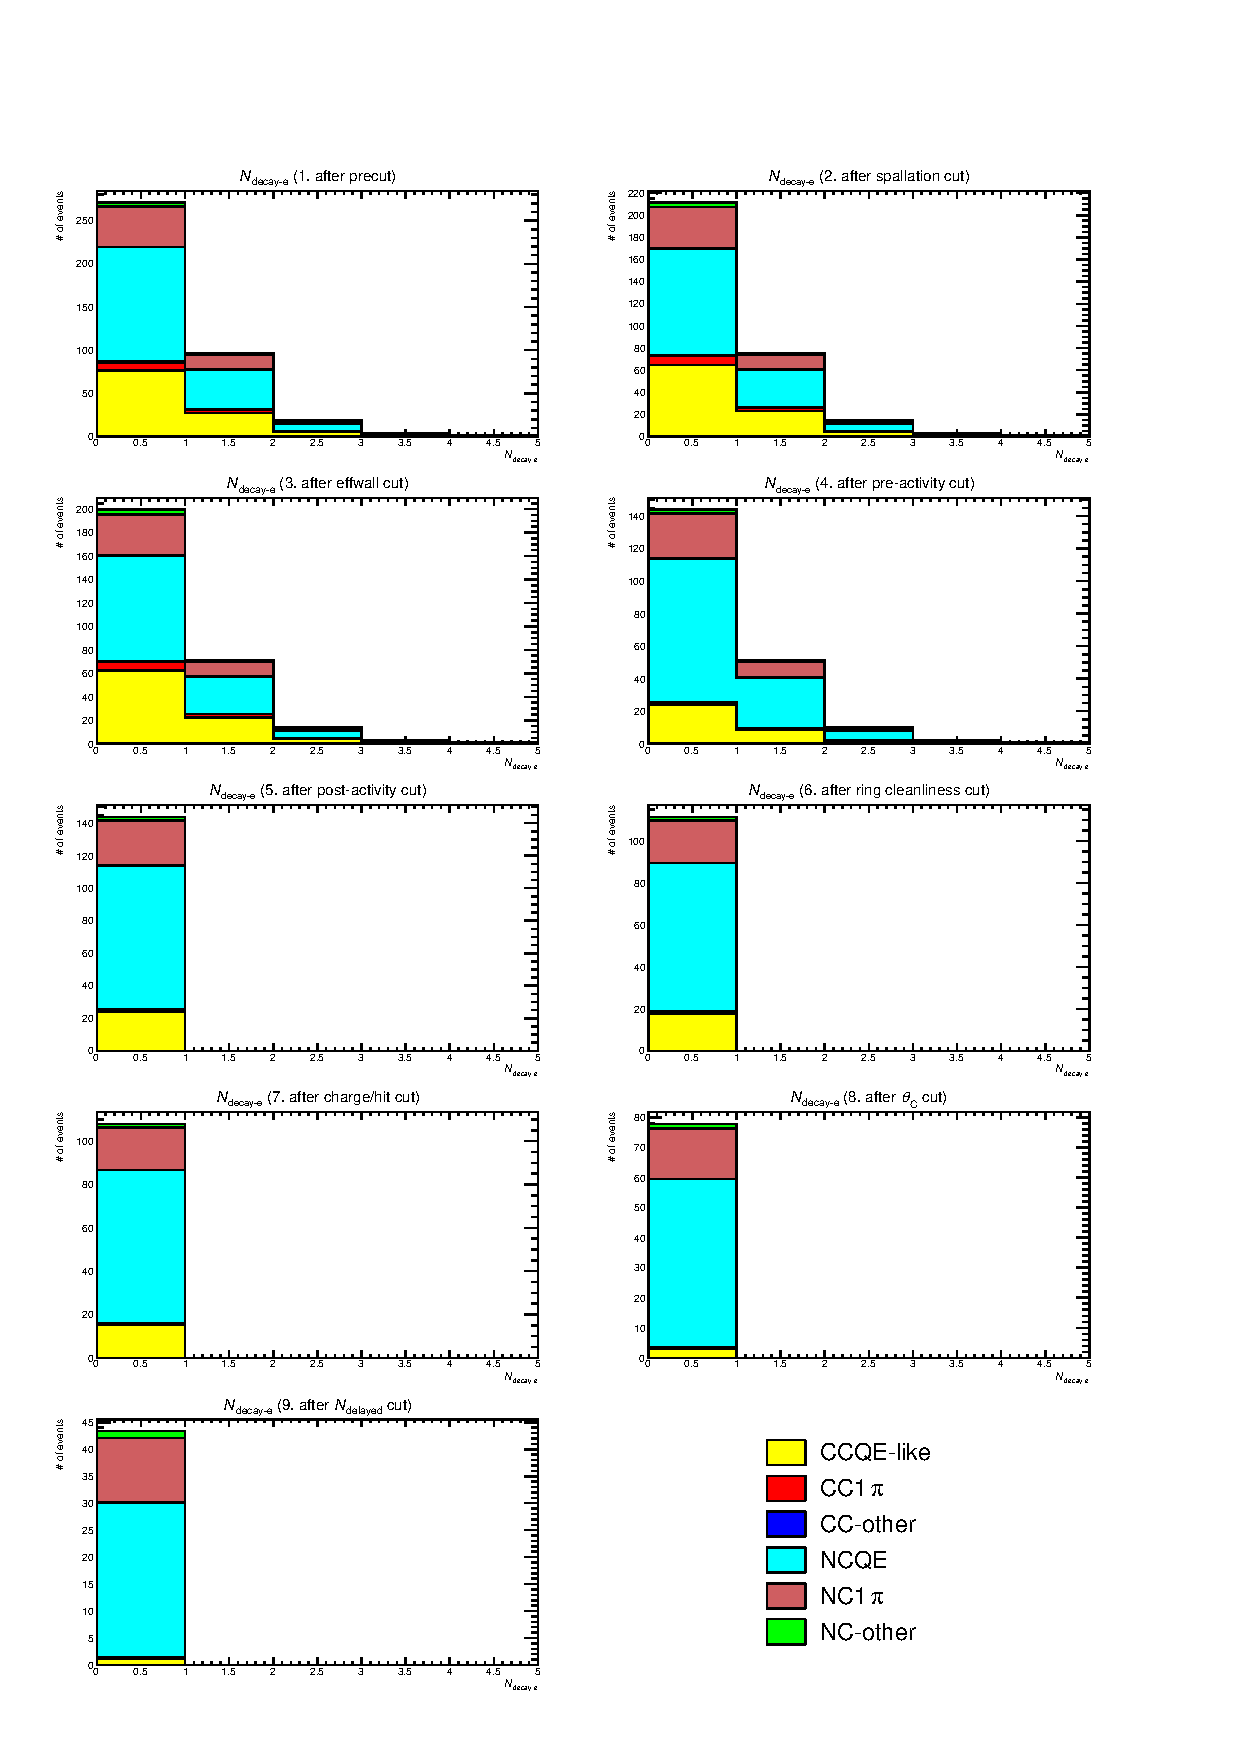
\includegraphics[width=15cm]{PDF/Dist_ATM/Che_50deg_tag_ge1/All/nmue}
	\caption[$N_{\rm decay\mathchar`-e}$ for atmospheric neutrino events]{
	$N_{\rm decay\mathchar`-e}$ for atmospheric neutrino events.
	Event reductions are performed in the order shown in the title.
	}\label{ATM_nmue}
\end{figure}

\begin{figure}[h]
	\centering
	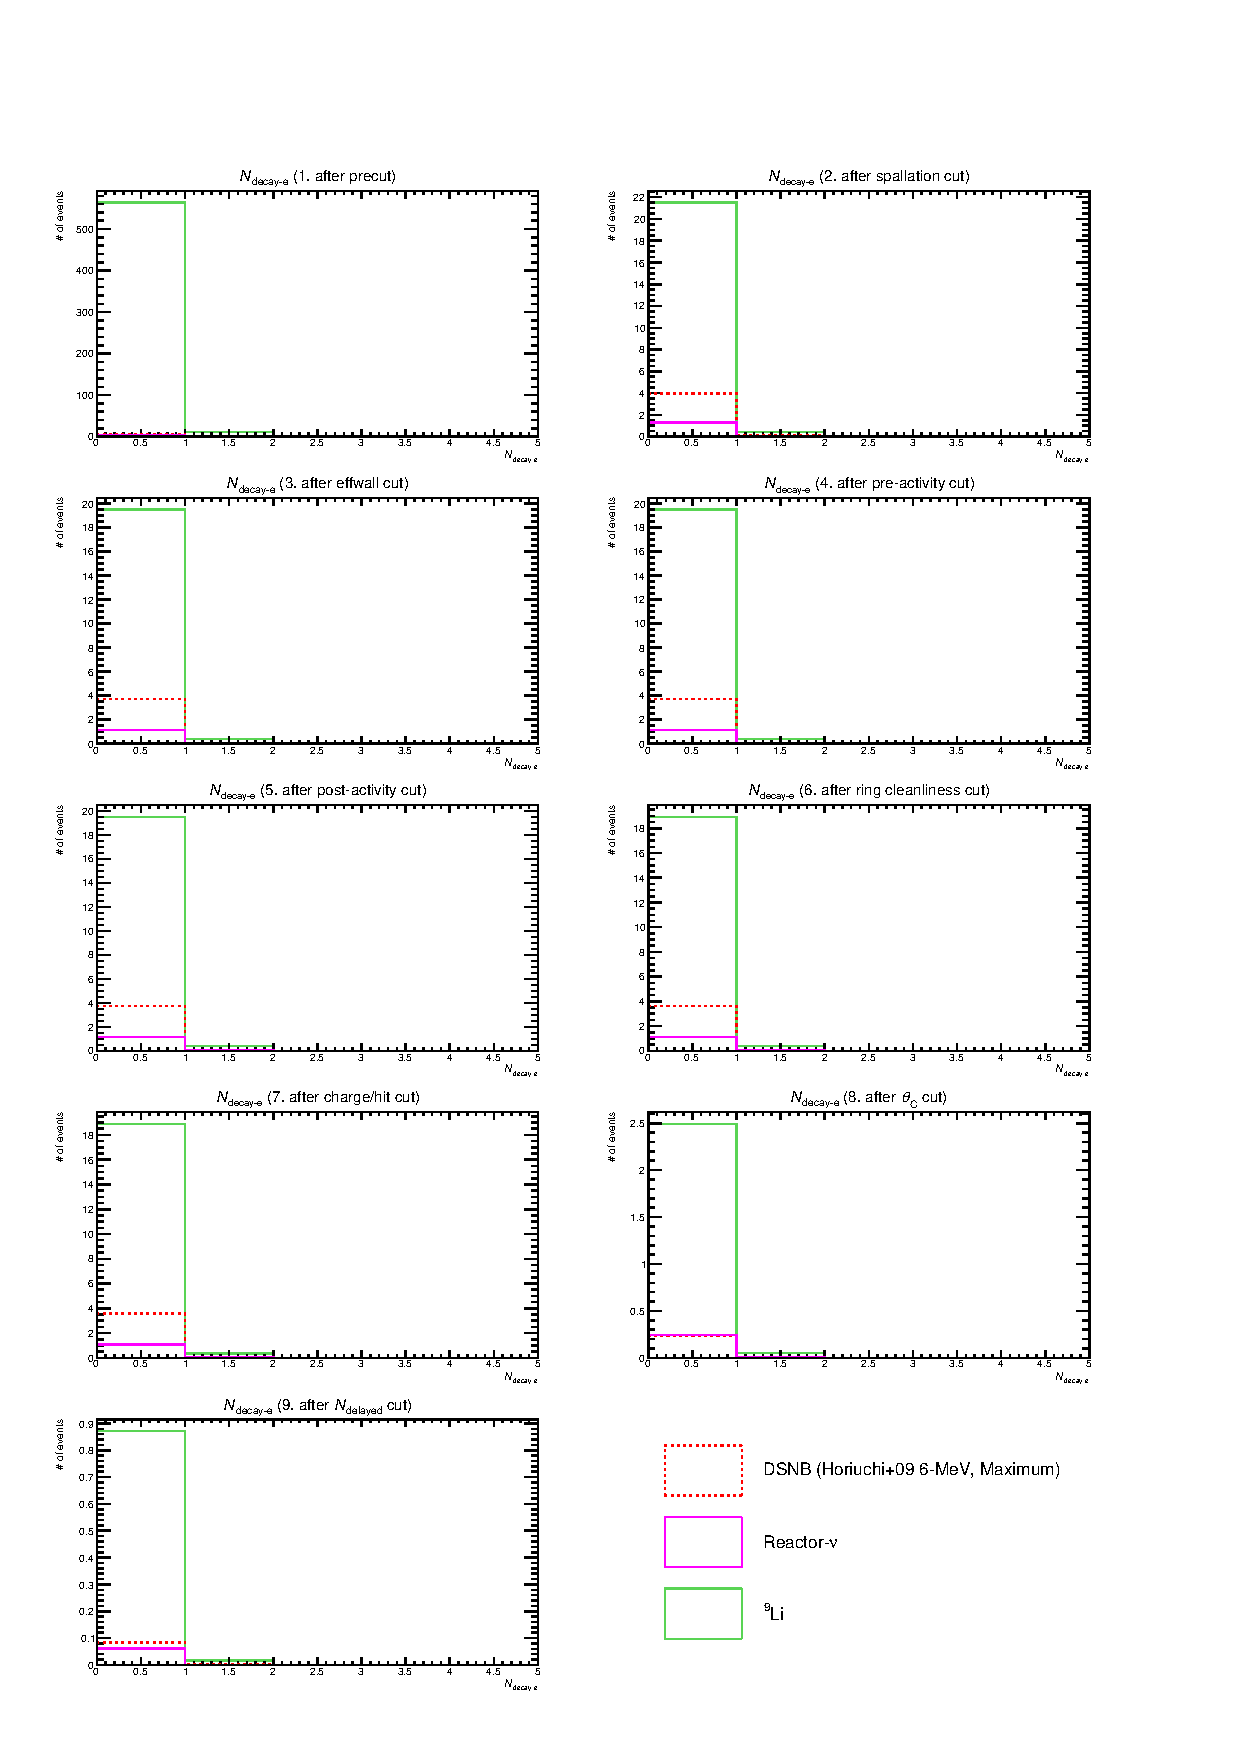
\includegraphics[width=15cm]{PDF/Dist_Nuebar/Che_50deg_tag_ge1/nmue}
	\caption[$N_{\rm decay\mathchar`-e}$ for spallation, reactor neutrino, and DSNB events]{
	$N_{\rm decay\mathchar`-e}$ for spallation, reactor neutrino, and DSNB events.
	Event reductions are performed in the order shown in the title.
	}\label{Nuebar_nmue}
\end{figure}

\begin{figure}[h]
	\centering
	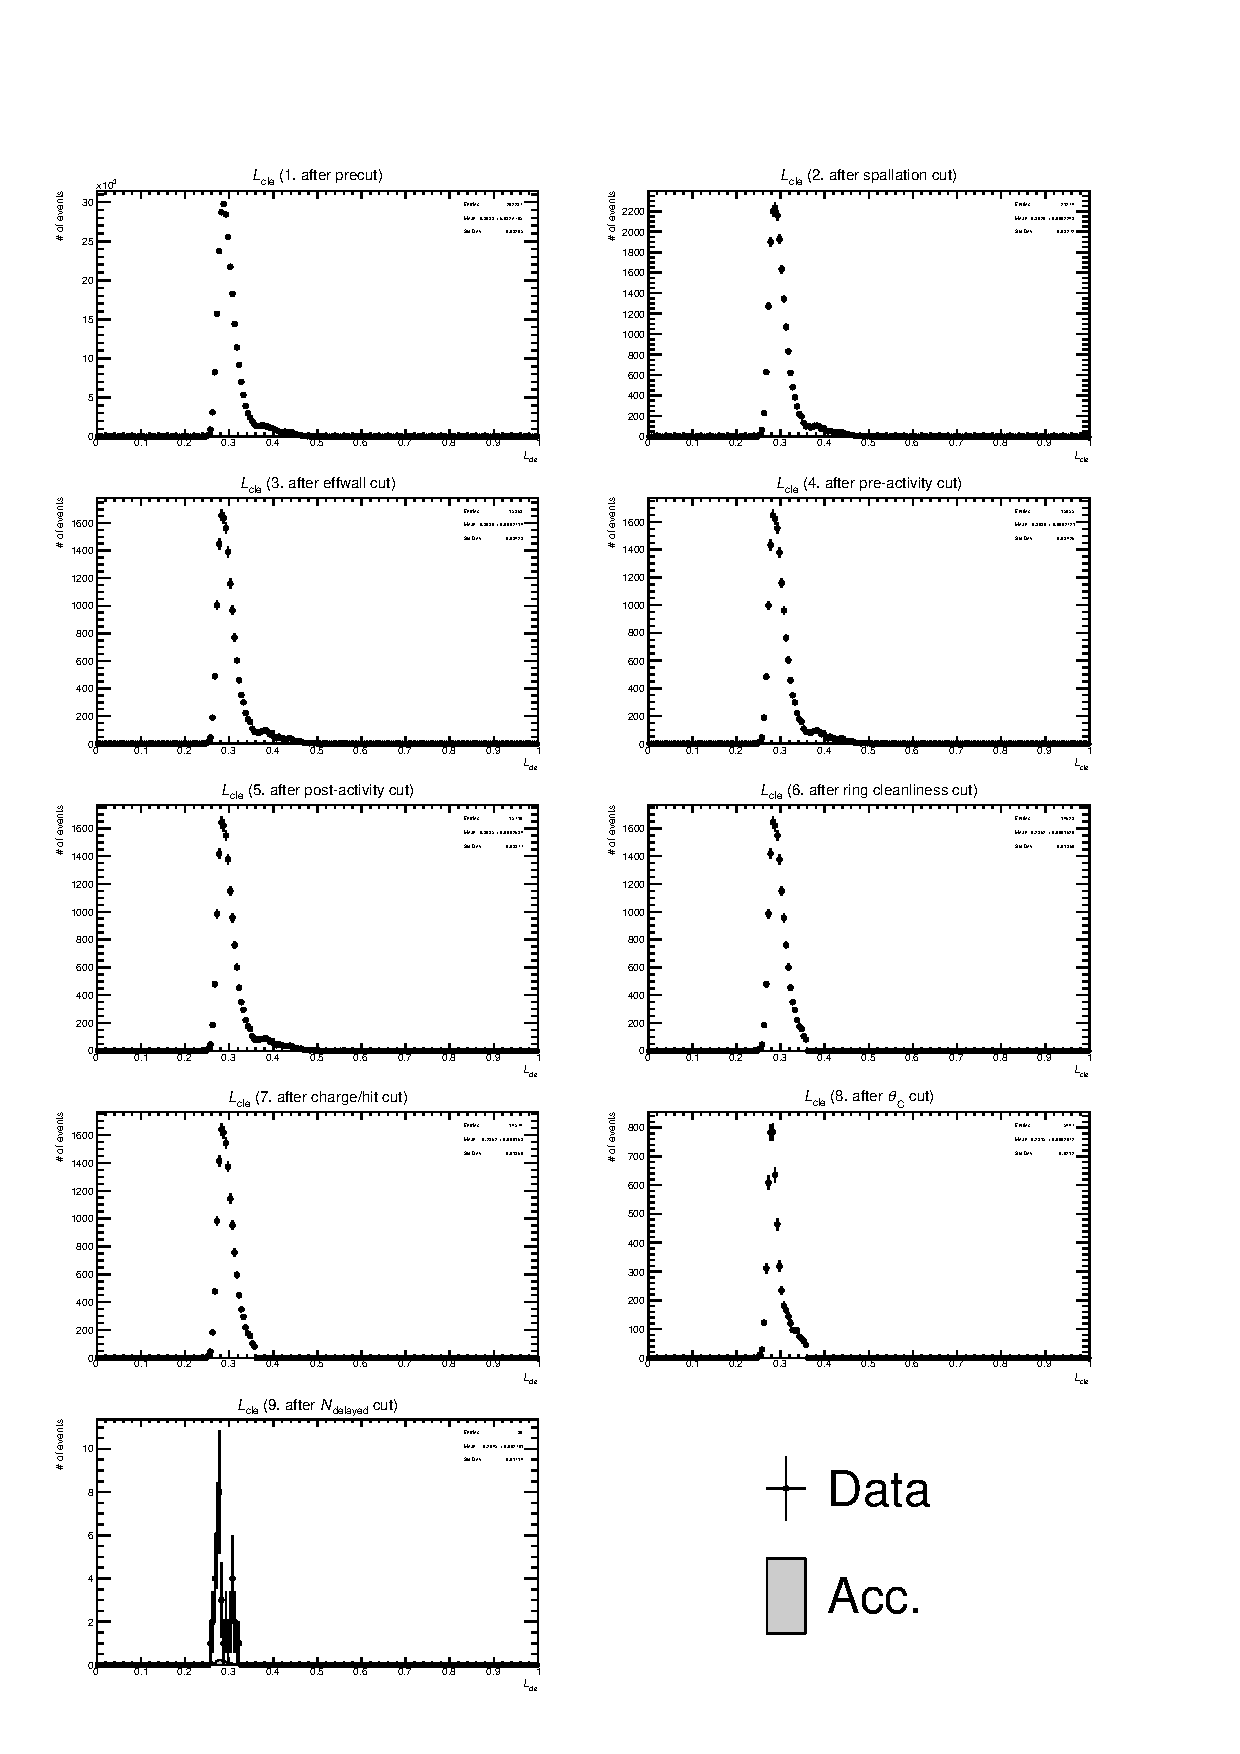
\includegraphics[width=15cm]{PDF/Dist_Data/Che_50deg_tag_ge1/pilike}
	\caption[$L_{\rm cle}$ for the data and accidental coincidence events]{
	$L_{\rm cle}$ for the data and accidental coincidence events.
	Event reductions are performed in the order shown in the title.
	}\label{Data_pilike}
\end{figure}

\begin{figure}[h]
	\centering
	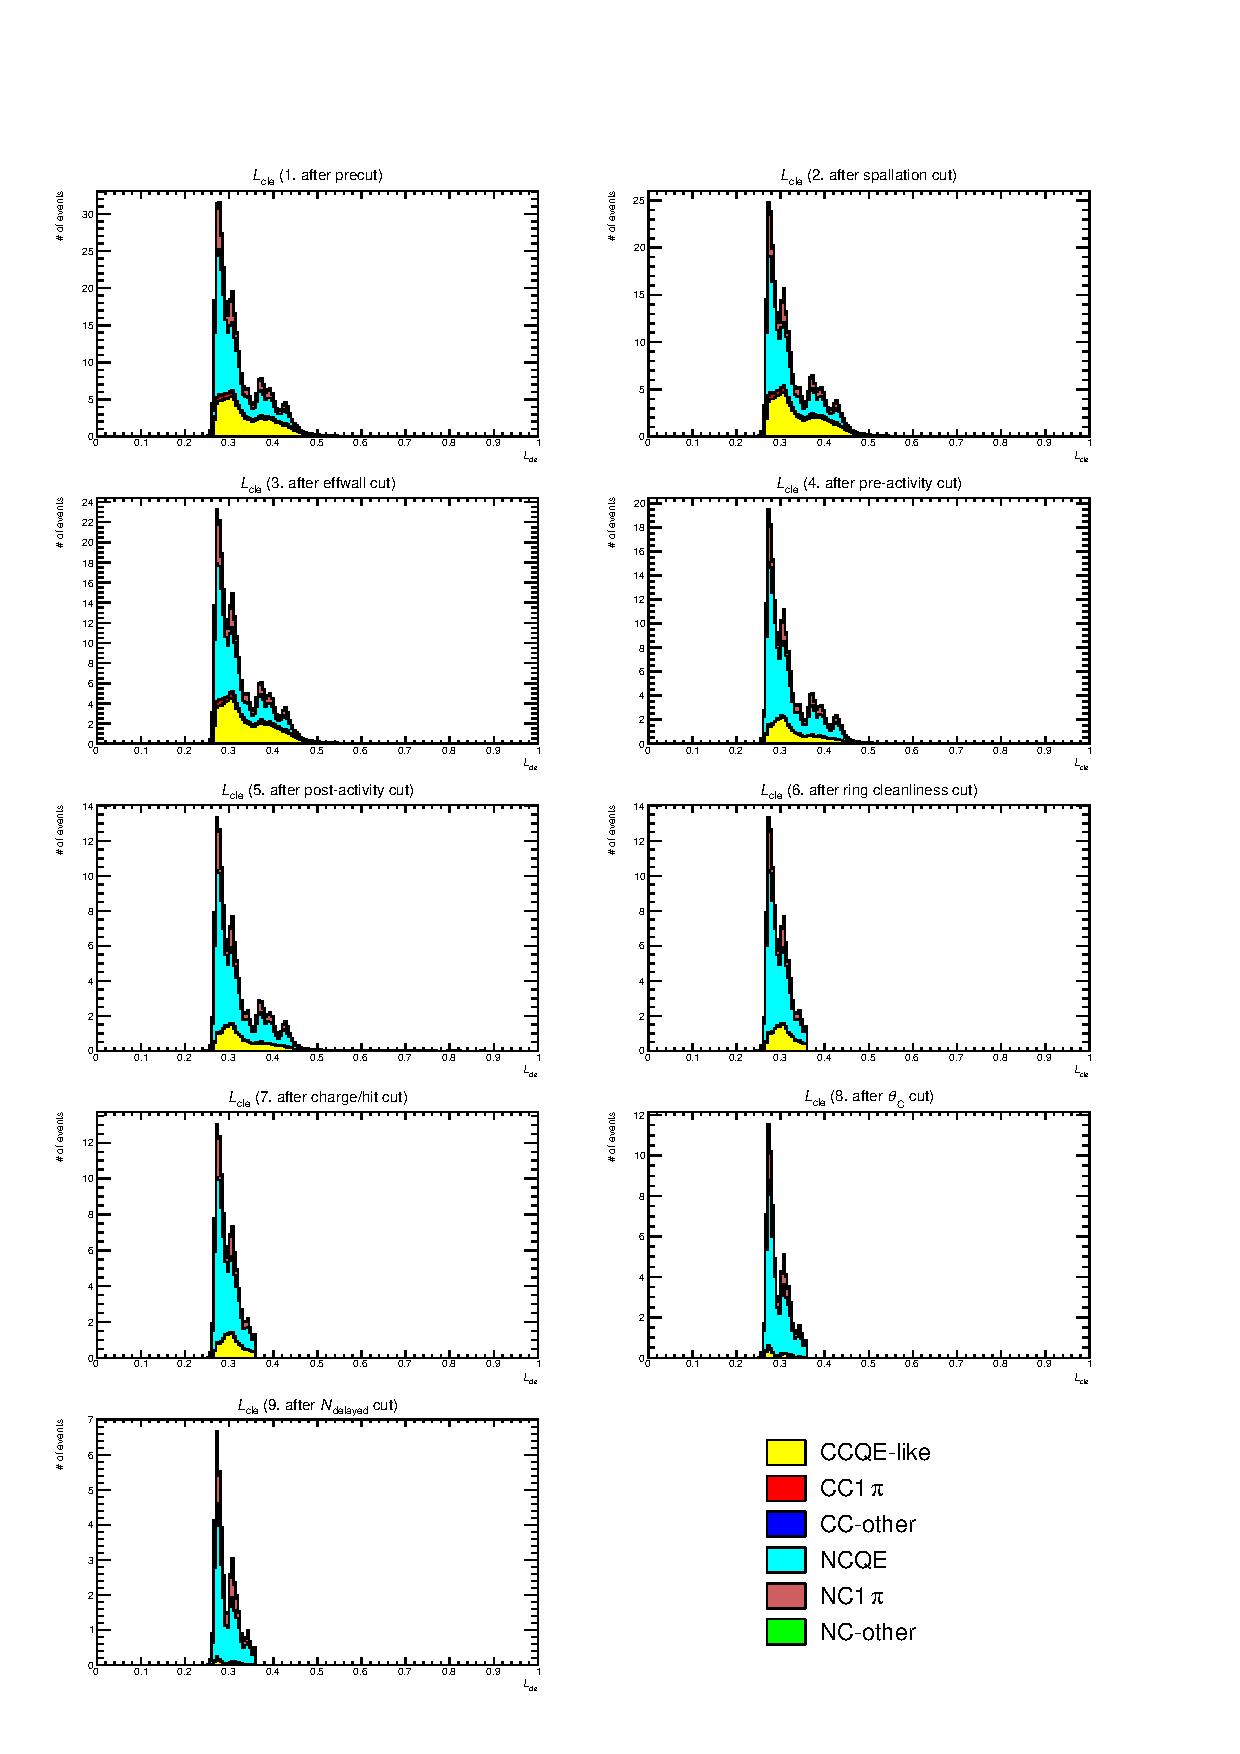
\includegraphics[width=15cm]{PDF/Dist_ATM/Che_50deg_tag_ge1/All/pilike}
	\caption[$L_{\rm cle}$ for atmospheric neutrino events]{
	$L_{\rm cle}$ for atmospheric neutrino events.
	Event reductions are performed in the order shown in the title.
	}\label{ATM_pilike}
\end{figure}

\begin{figure}[h]
	\centering
	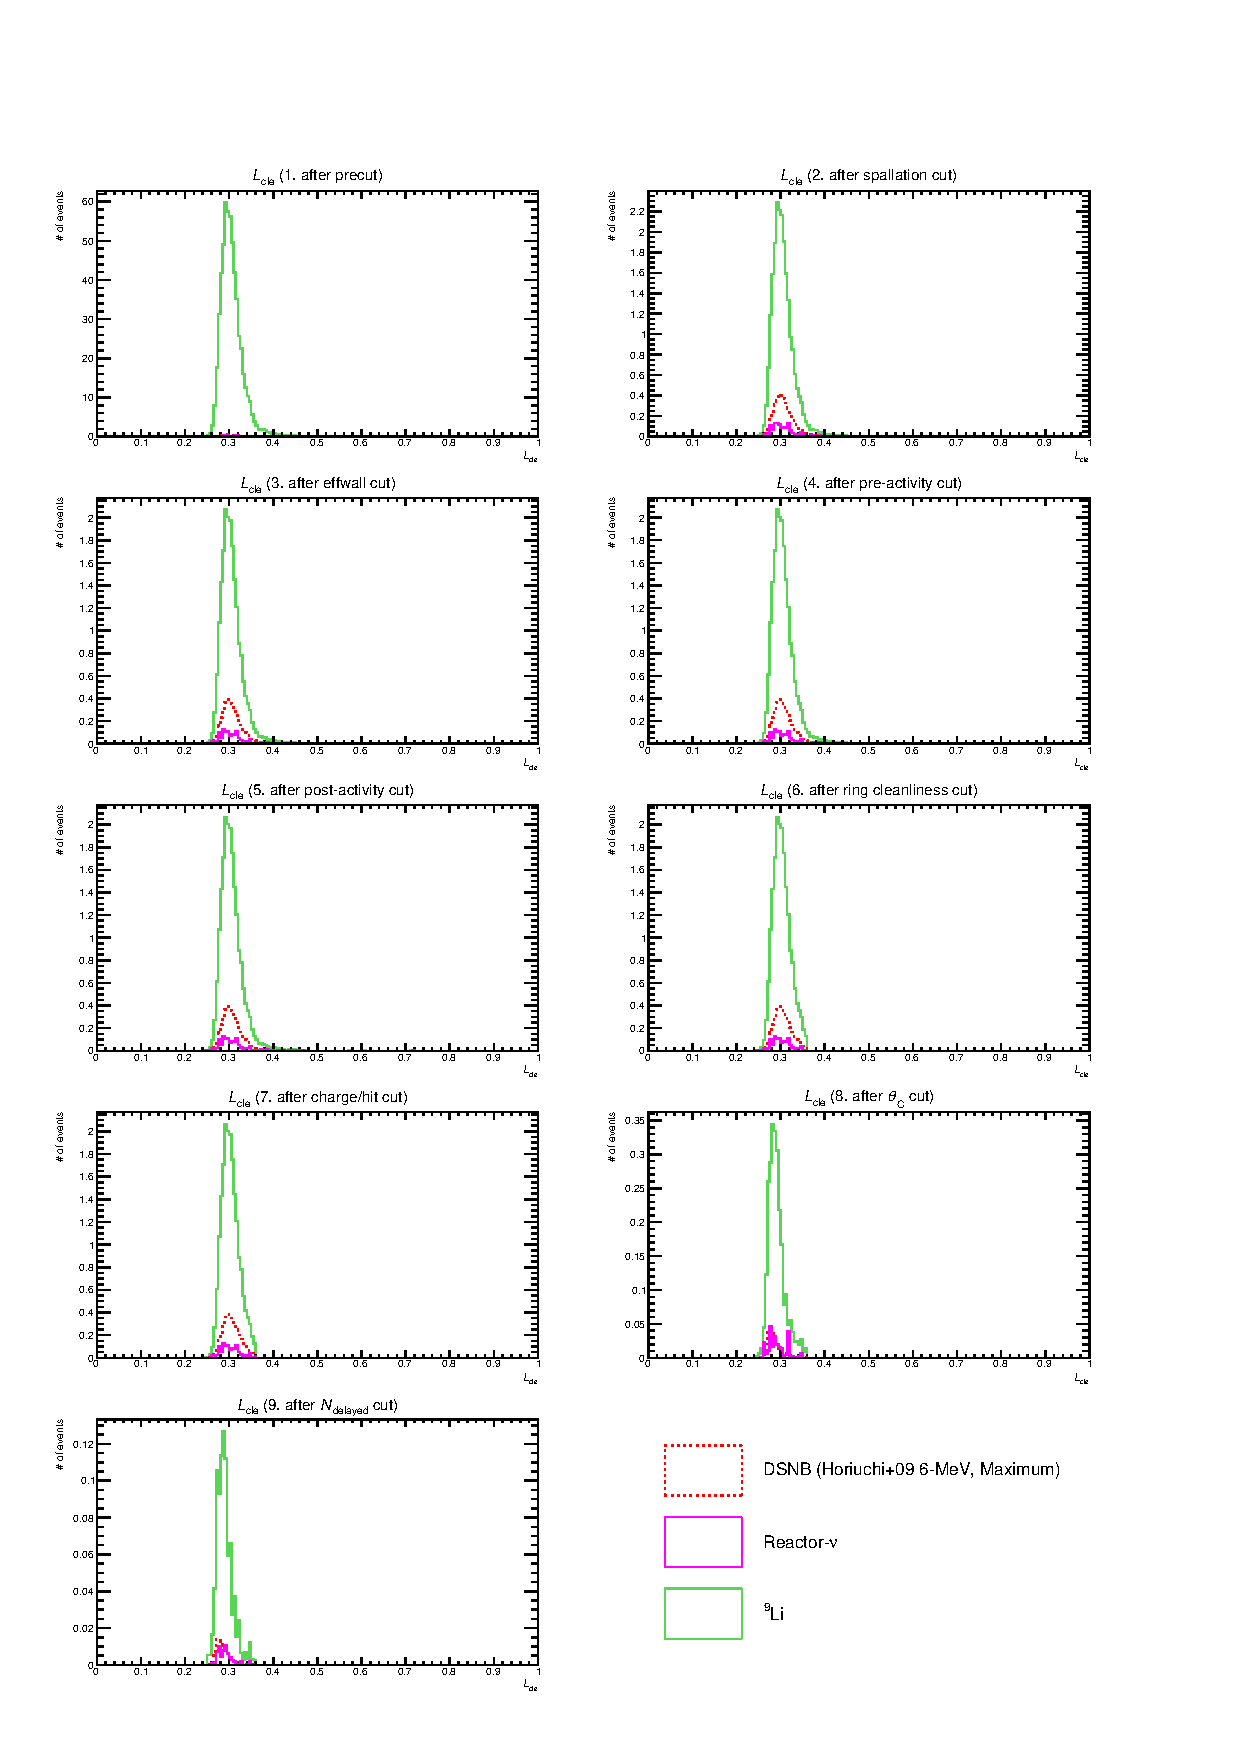
\includegraphics[width=15cm]{PDF/Dist_Nuebar/Che_50deg_tag_ge1/pilike}
	\caption[$L_{\rm cle}$ for spallation, reactor neutrino, and DSNB events]{
	$L_{\rm cle}$ for spallation, reactor neutrino, and DSNB events.
	Event reductions are performed in the order shown in the title.
	}\label{Nuebar_pilike}
\end{figure}

\begin{figure}[h]
	\centering
	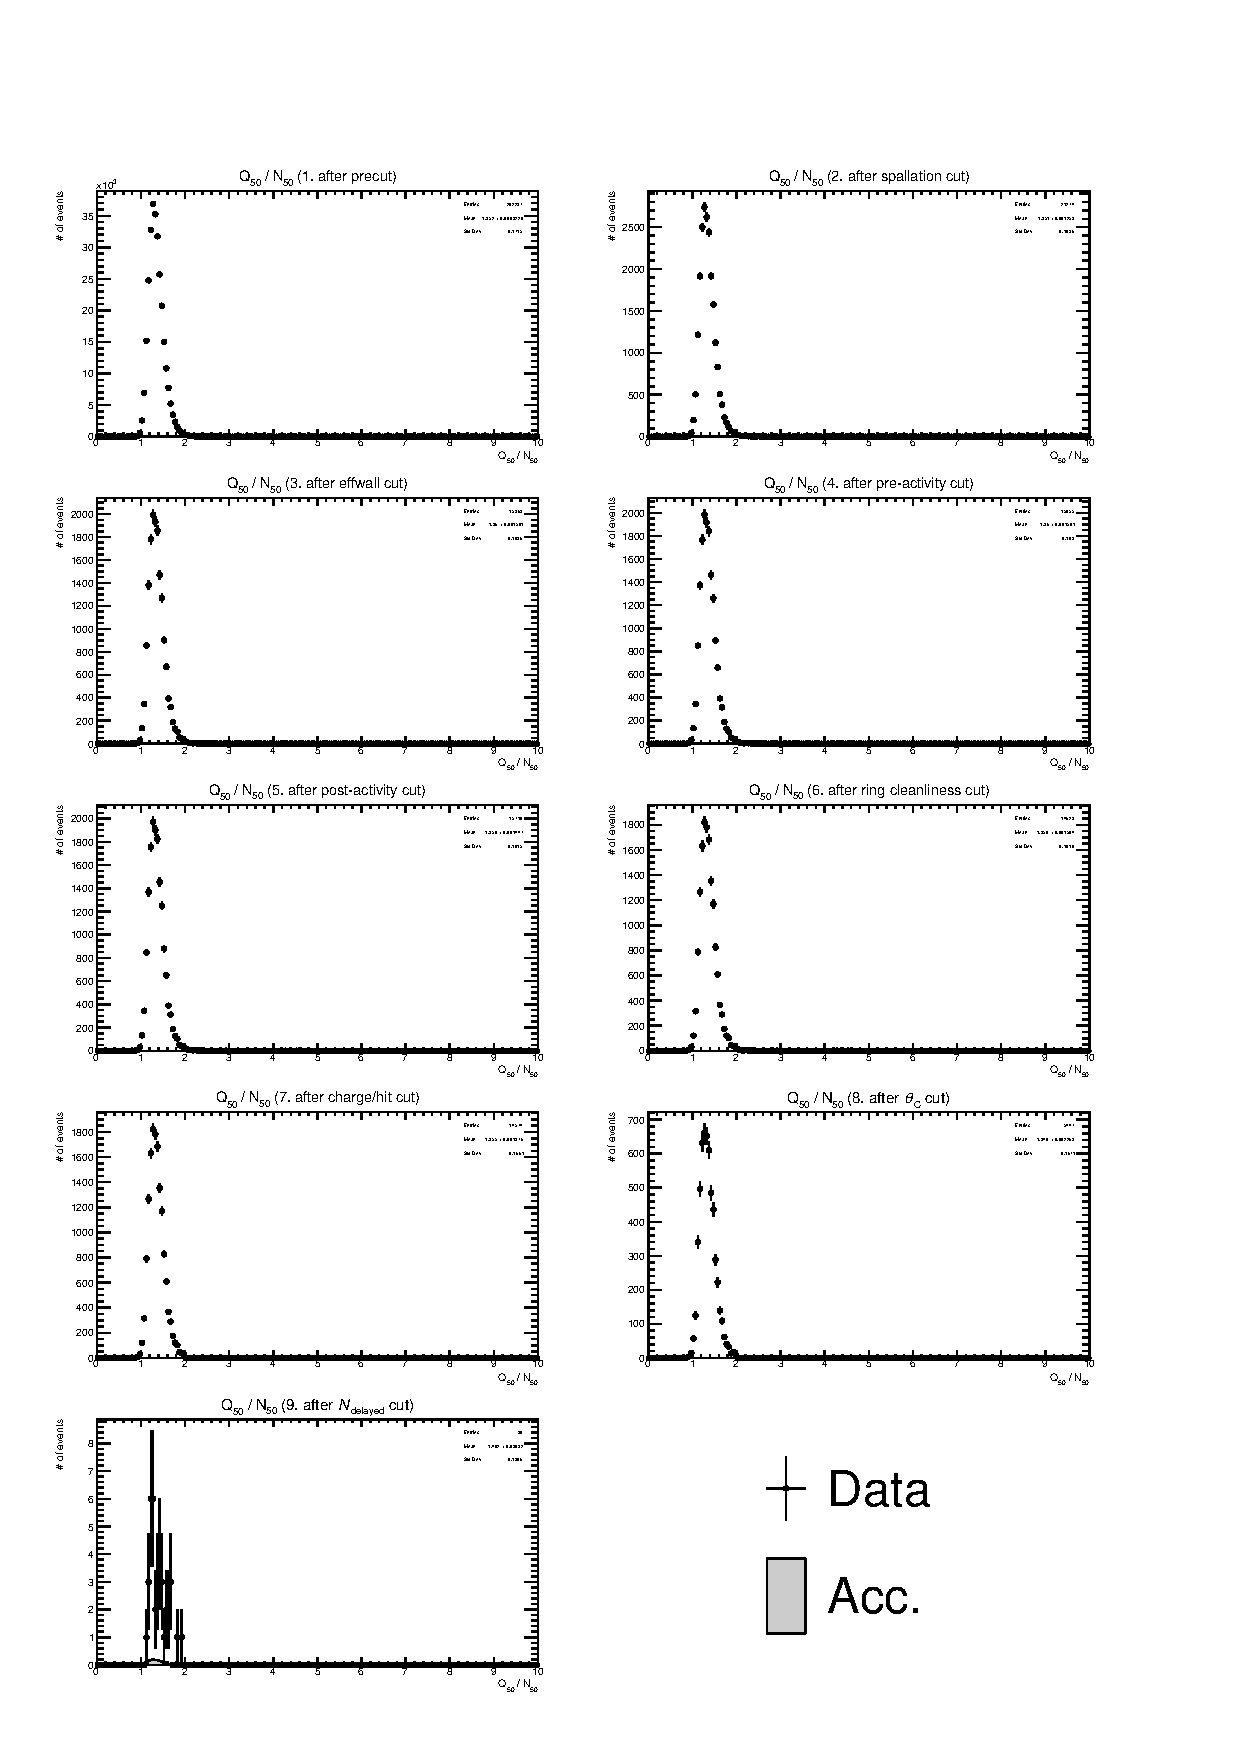
\includegraphics[width=15cm]{PDF/Dist_Data/Che_50deg_tag_ge1/q50n50}
	\caption[$Q_{50}/N_{50}$ for the data and accidental coincidence events]{
	$Q_{50}/N_{50}$ for the data and accidental coincidence events.
	Event reductions are performed in the order shown in the title.
	}\label{Data_q50n50}
\end{figure}

\begin{figure}[h]
	\centering
	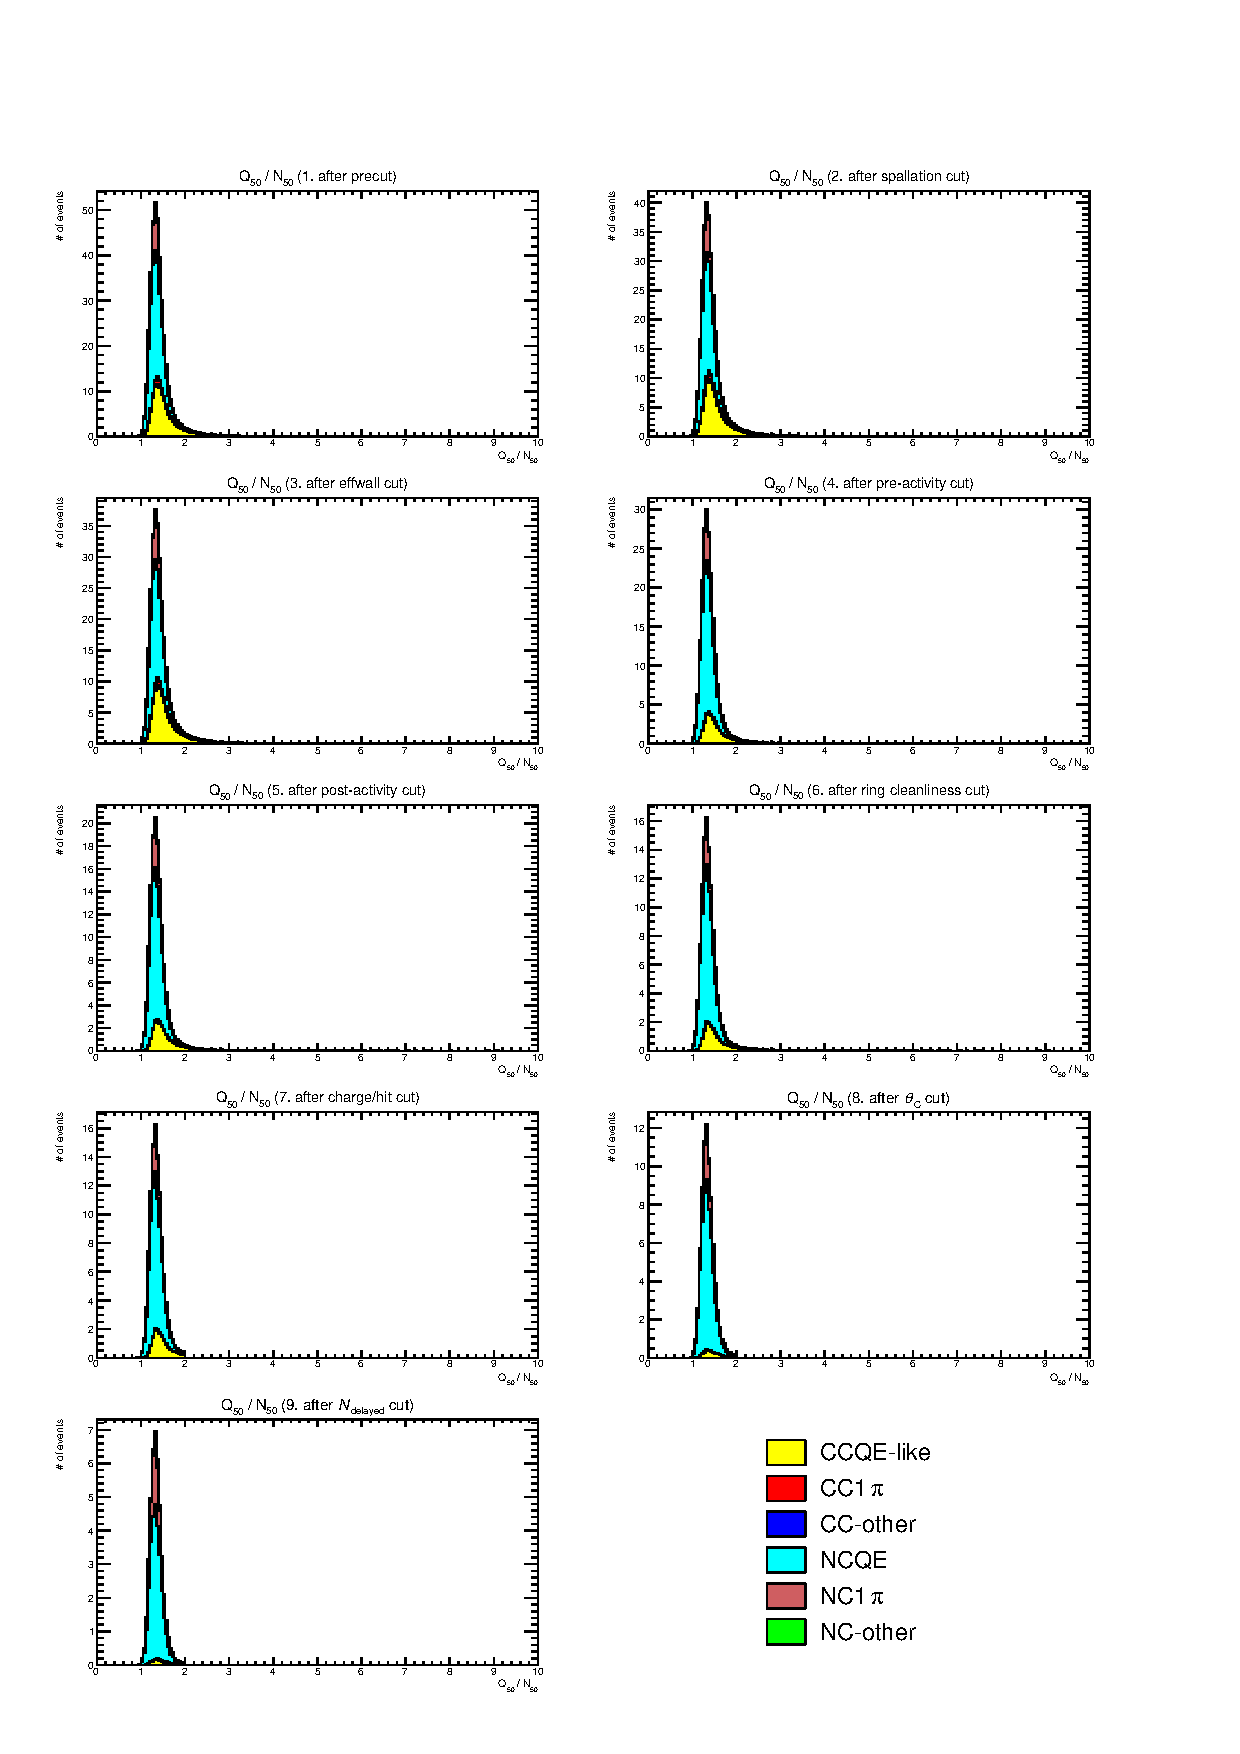
\includegraphics[width=15cm]{PDF/Dist_ATM/Che_50deg_tag_ge1/All/q50n50}
	\caption[$Q_{50}/N_{50}$ for atmospheric neutrino events]{
	$Q_{50}/N_{50}$ for atmospheric neutrino events.
	Event reductions are performed in the order shown in the title.
	}\label{ATM_q50n50}
\end{figure}

\begin{figure}[h]
	\centering
	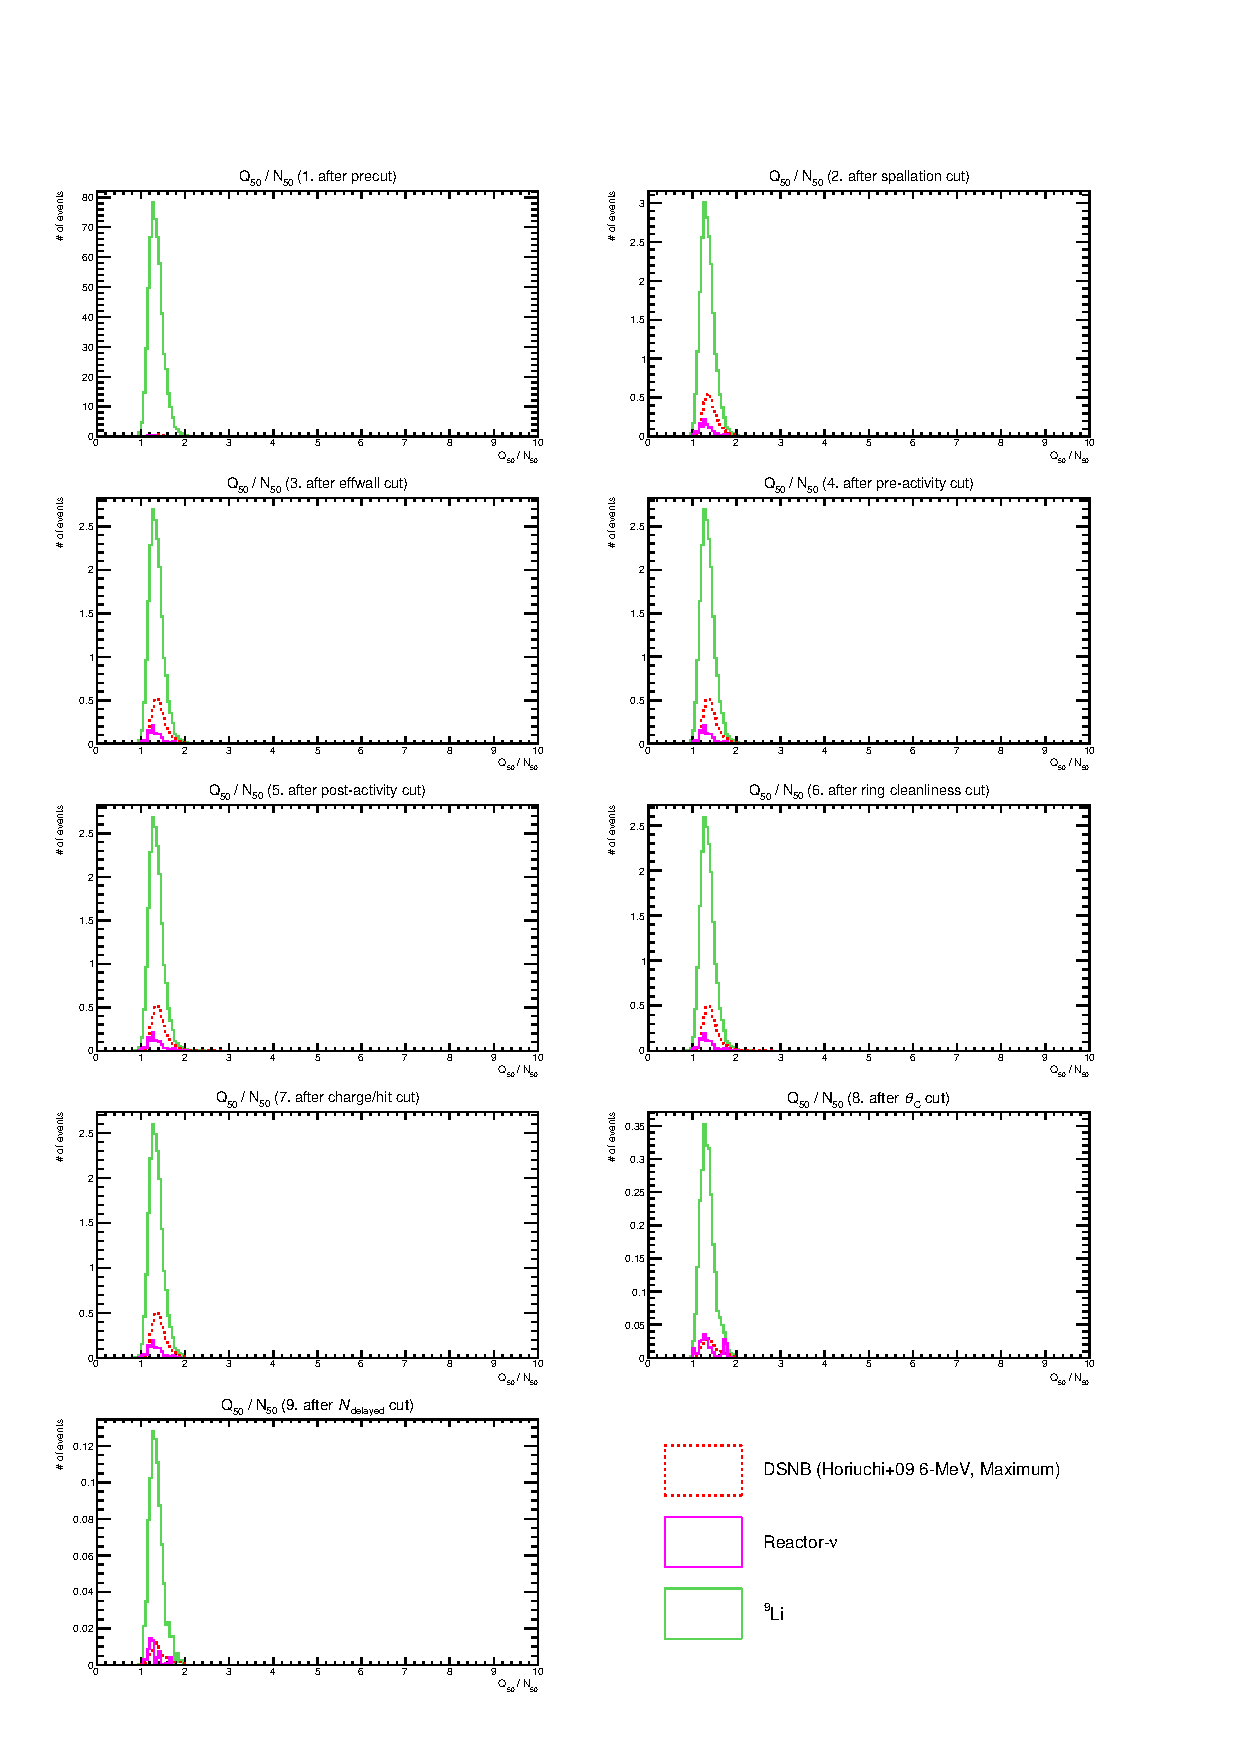
\includegraphics[width=15cm]{PDF/Dist_Nuebar/Che_50deg_tag_ge1/q50n50}
	\caption[$Q_{50}/N_{50}$ for spallation, reactor neutrino, and DSNB events]{
	$Q_{50}/N_{50}$ for spallation, reactor neutrino, and DSNB events.
	Event reductions are performed in the order shown in the title.
	}\label{Nuebar_q50n50}
\end{figure}

\begin{figure}[h]
	\centering
	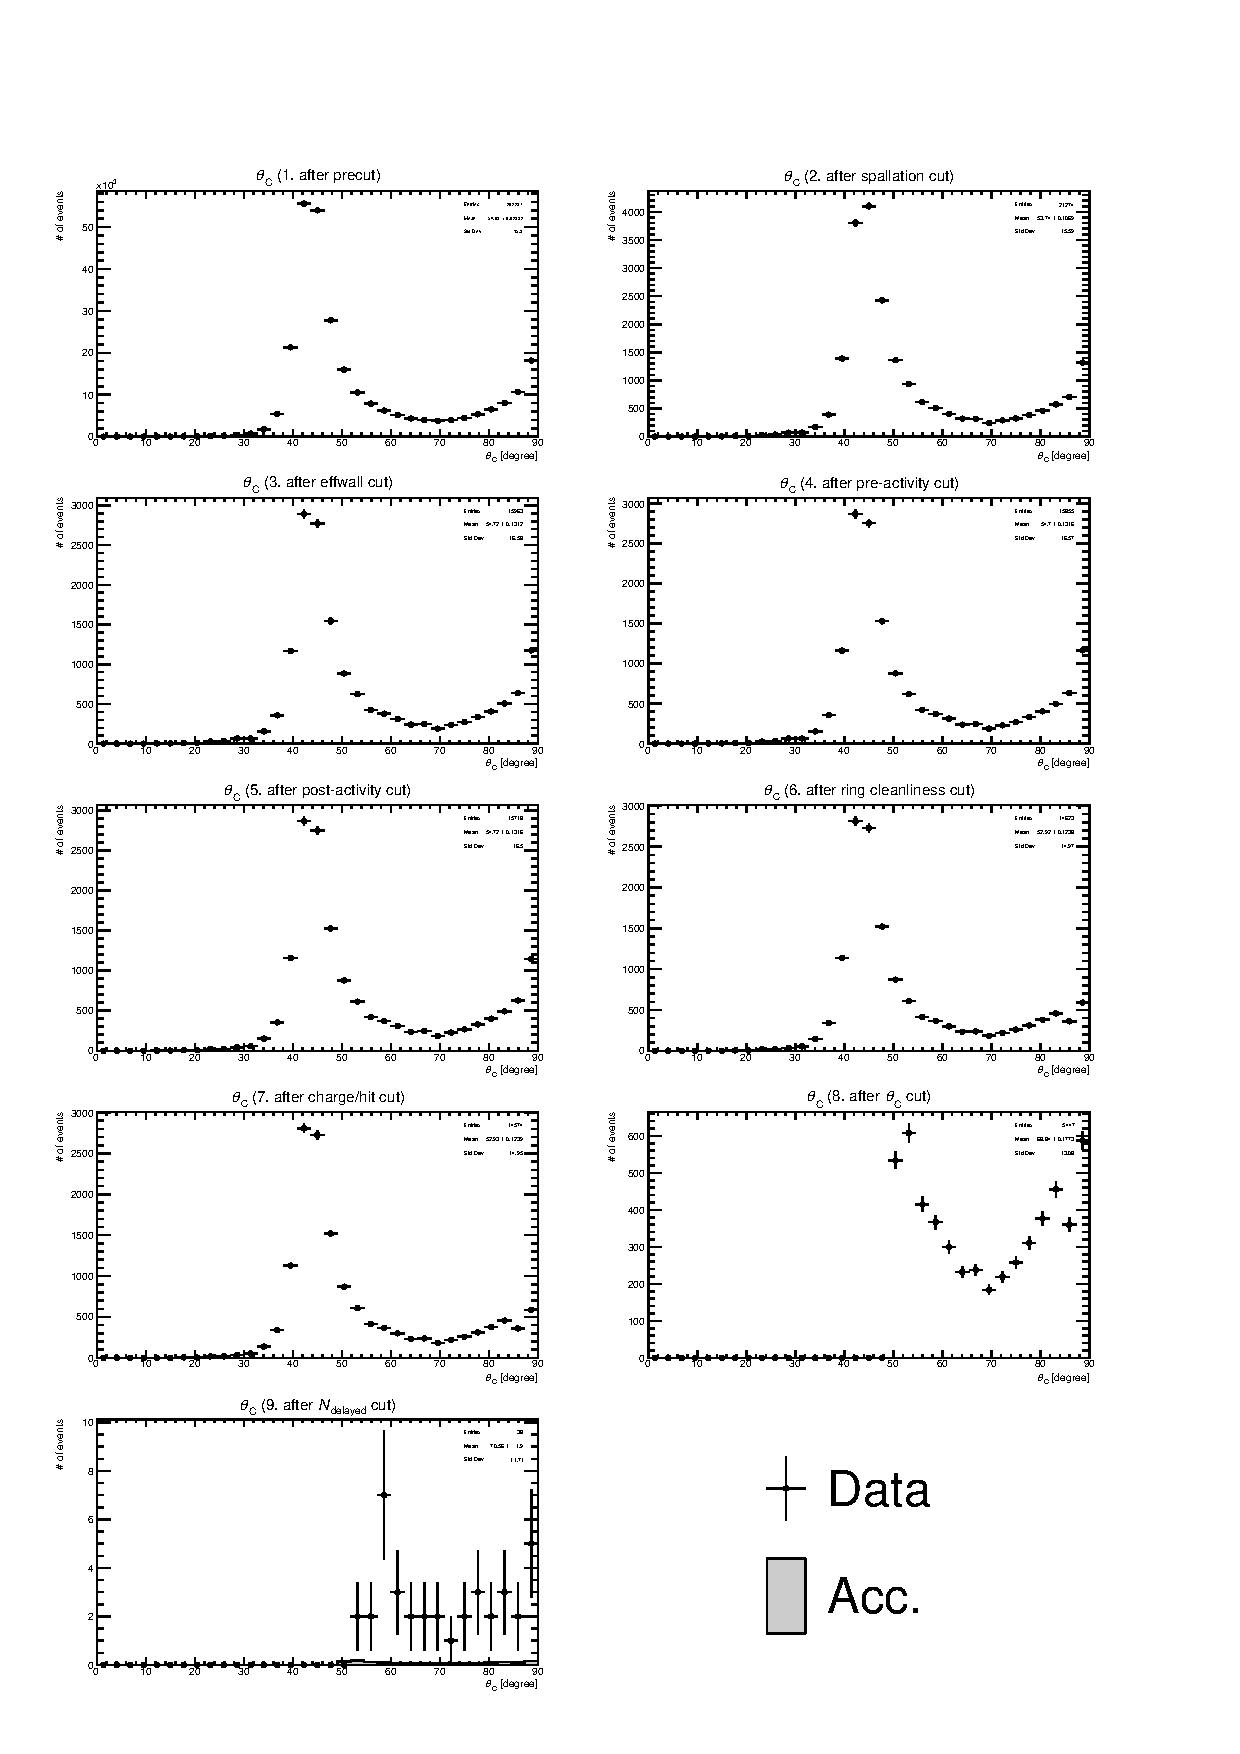
\includegraphics[width=15cm]{PDF/Dist_Data/Che_50deg_tag_ge1/angle}
	\caption[$\theta_{\rm C}$ for the data and accidental coincidence events]{
	$\theta_{\rm C}$ for the data and accidental coincidence events.
	Event reductions are performed in the order shown in the title.
	}\label{Data_angle}
\end{figure}

\begin{figure}[h]
	\centering
	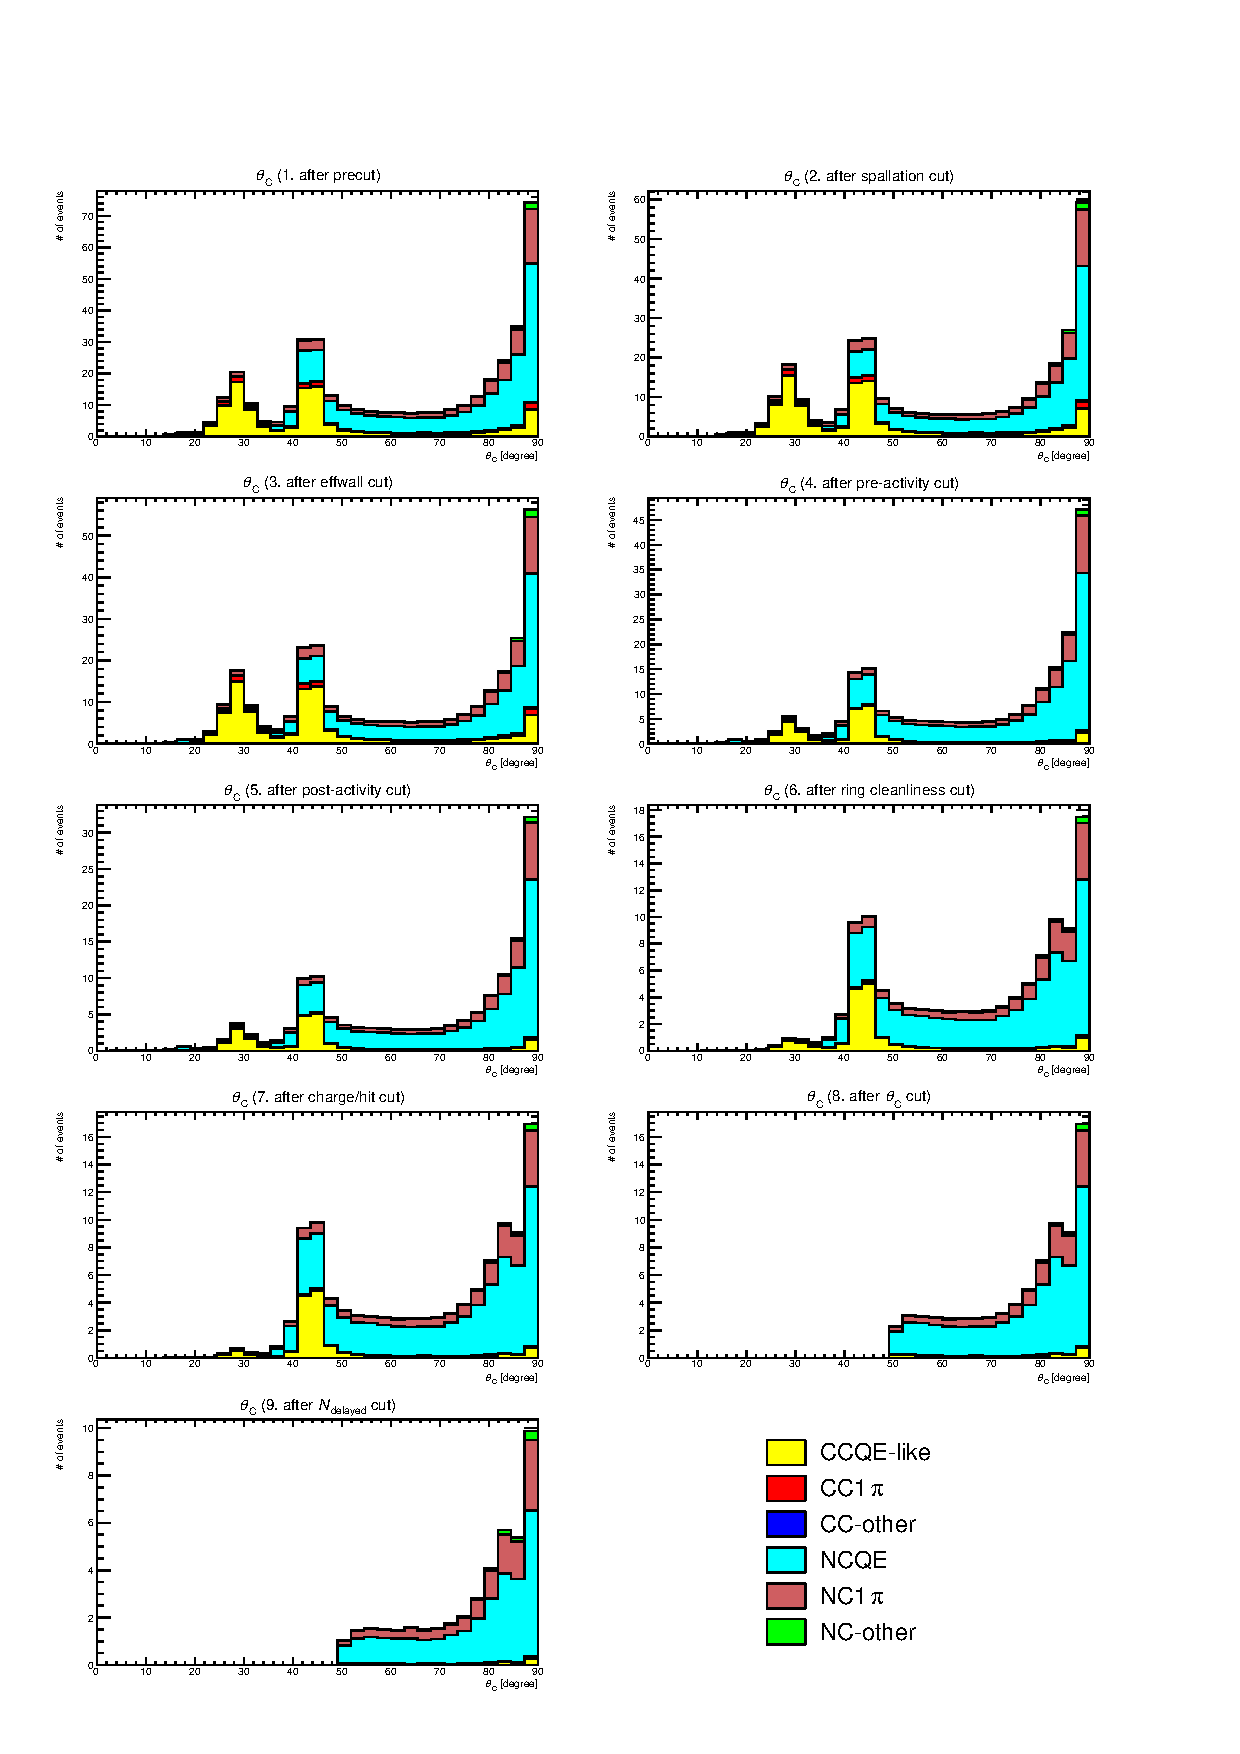
\includegraphics[width=15cm]{PDF/Dist_ATM/Che_50deg_tag_ge1/All/angle}
	\caption[$\theta_{\rm C}$ for atmospheric neutrino events]{
	$\theta_{\rm C}$ for atmospheric neutrino events.
	Event reductions are performed in the order shown in the title.
	}\label{ATM_angle}
\end{figure}

\begin{figure}[h]
	\centering
	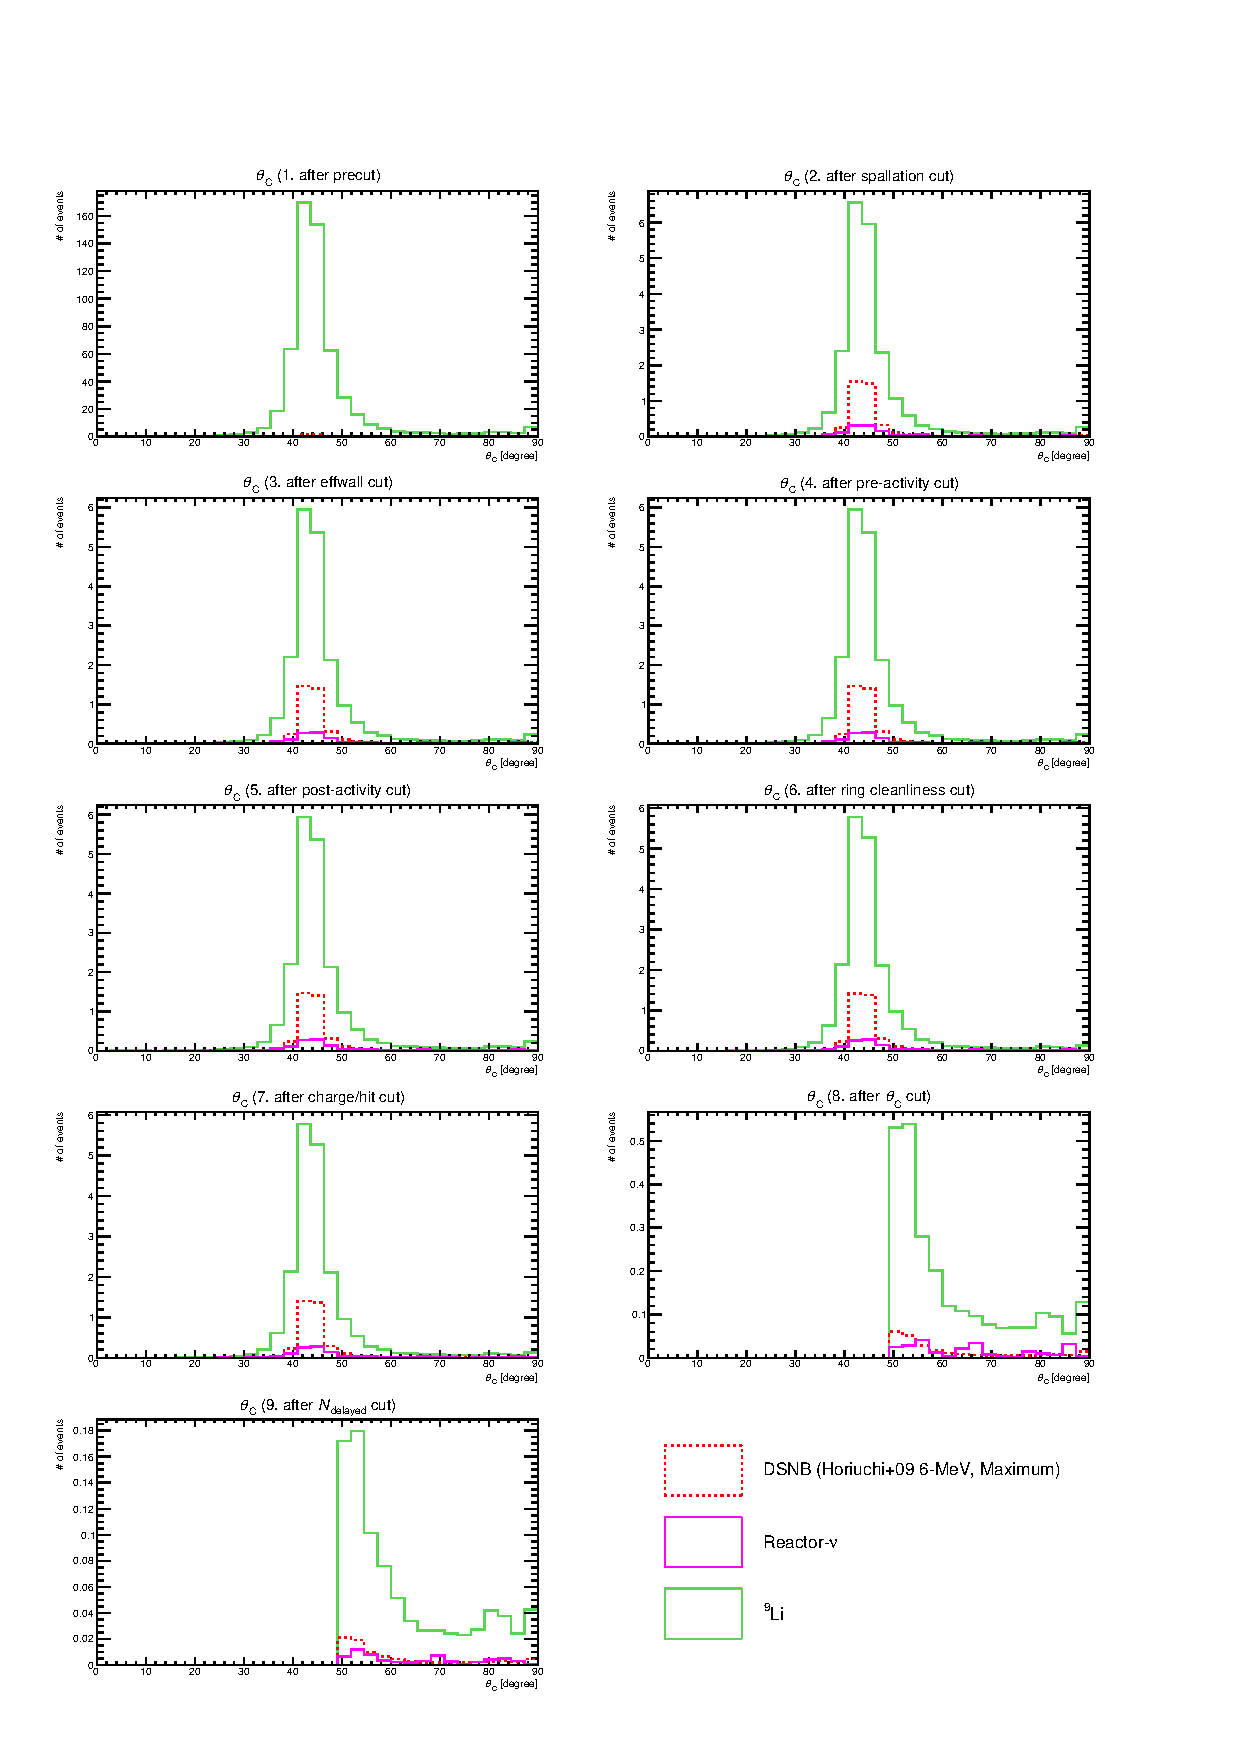
\includegraphics[width=15cm]{PDF/Dist_Nuebar/Che_50deg_tag_ge1/angle}
	\caption[$\theta_{\rm C}$ for spallation, reactor neutrino, and DSNB events]{
	$\theta_{\rm C}$ for spallation, reactor neutrino, and DSNB events.
	Event reductions are performed in the order shown in the title.
	}\label{Nuebar_angle}
\end{figure}

\begin{figure}[h]
	\centering
	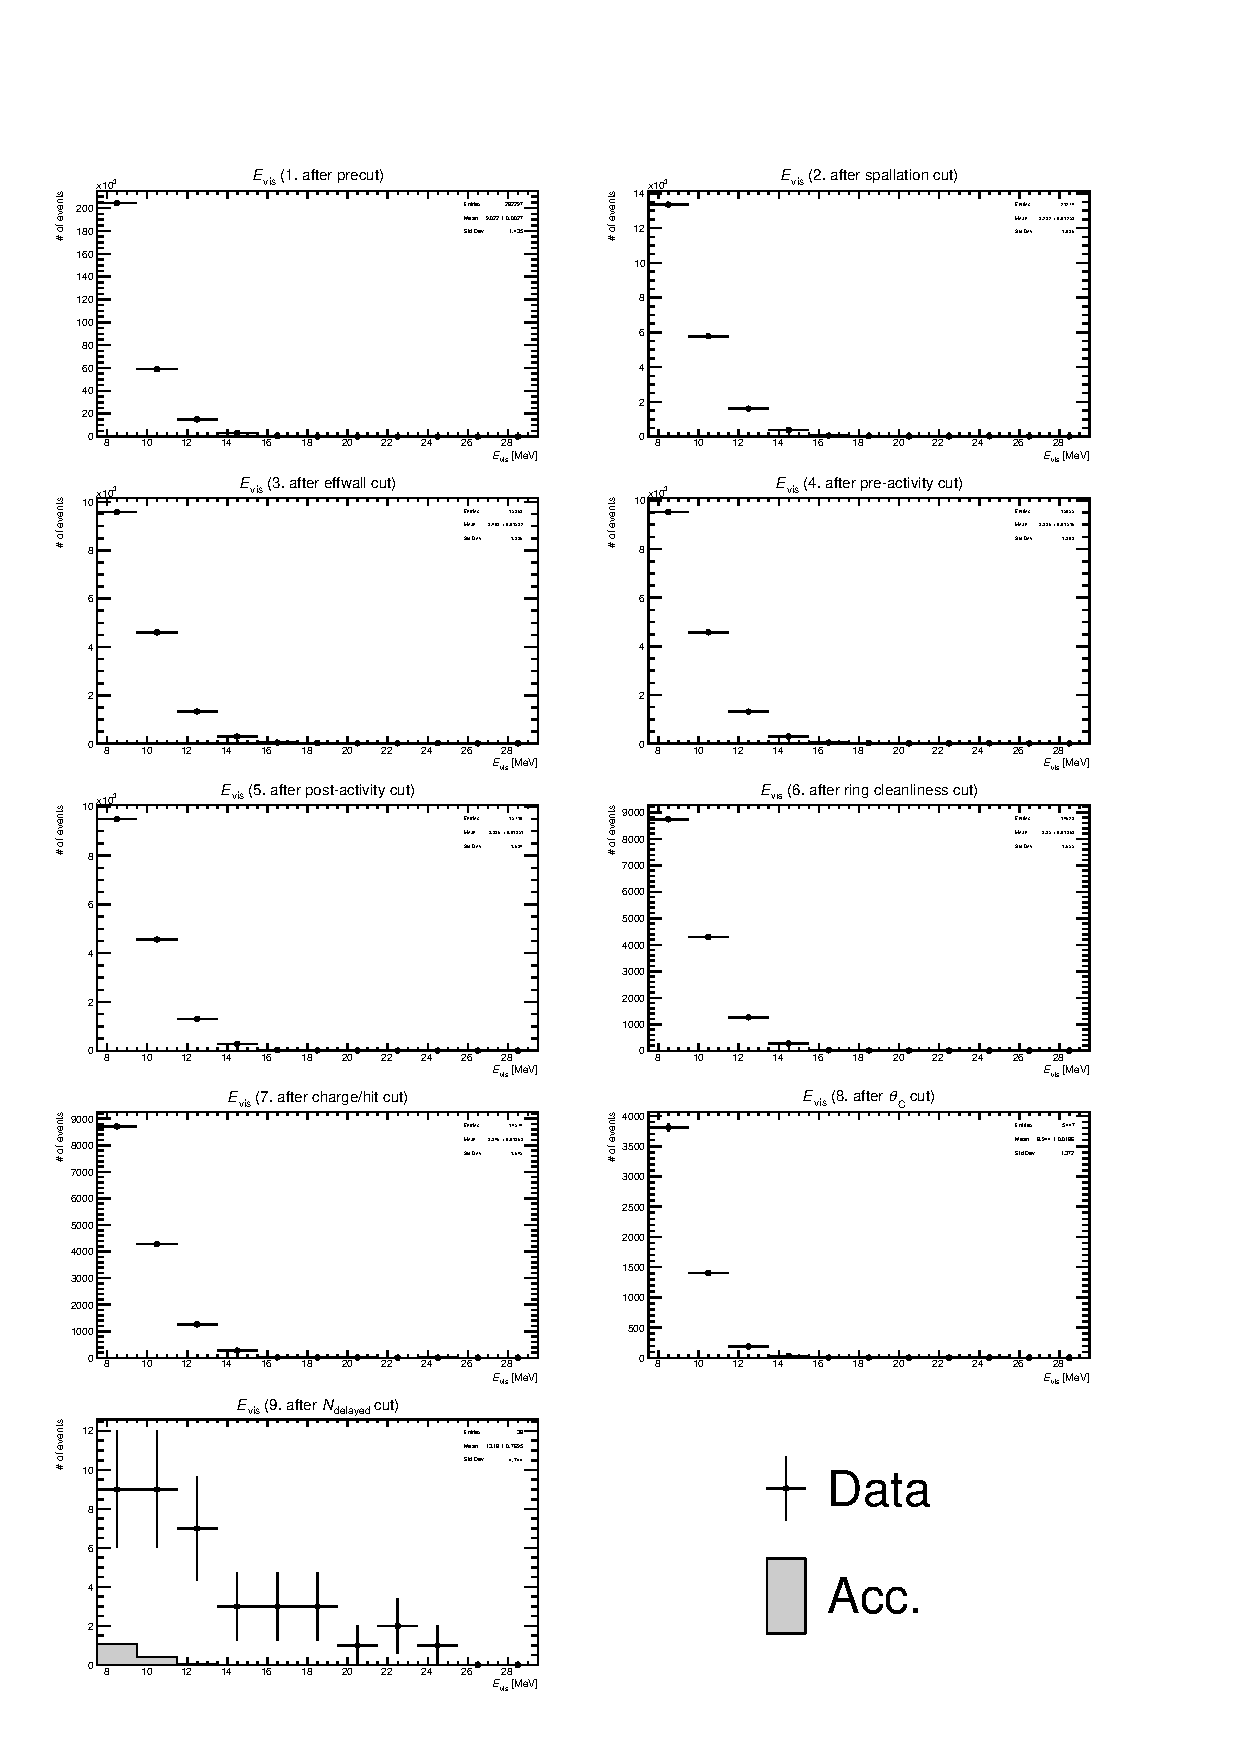
\includegraphics[width=15cm]{PDF/Dist_Data/Che_50deg_tag_ge1/erec}
	\caption[$E_{\rm vis}$ for the data and accidental coincidence events]{
	$E_{\rm vis}$ for the data and accidental coincidence events.
	Event reductions are performed in the order shown in the title.
	}\label{Data_erec}
\end{figure}

\begin{figure}[h]
	\centering
	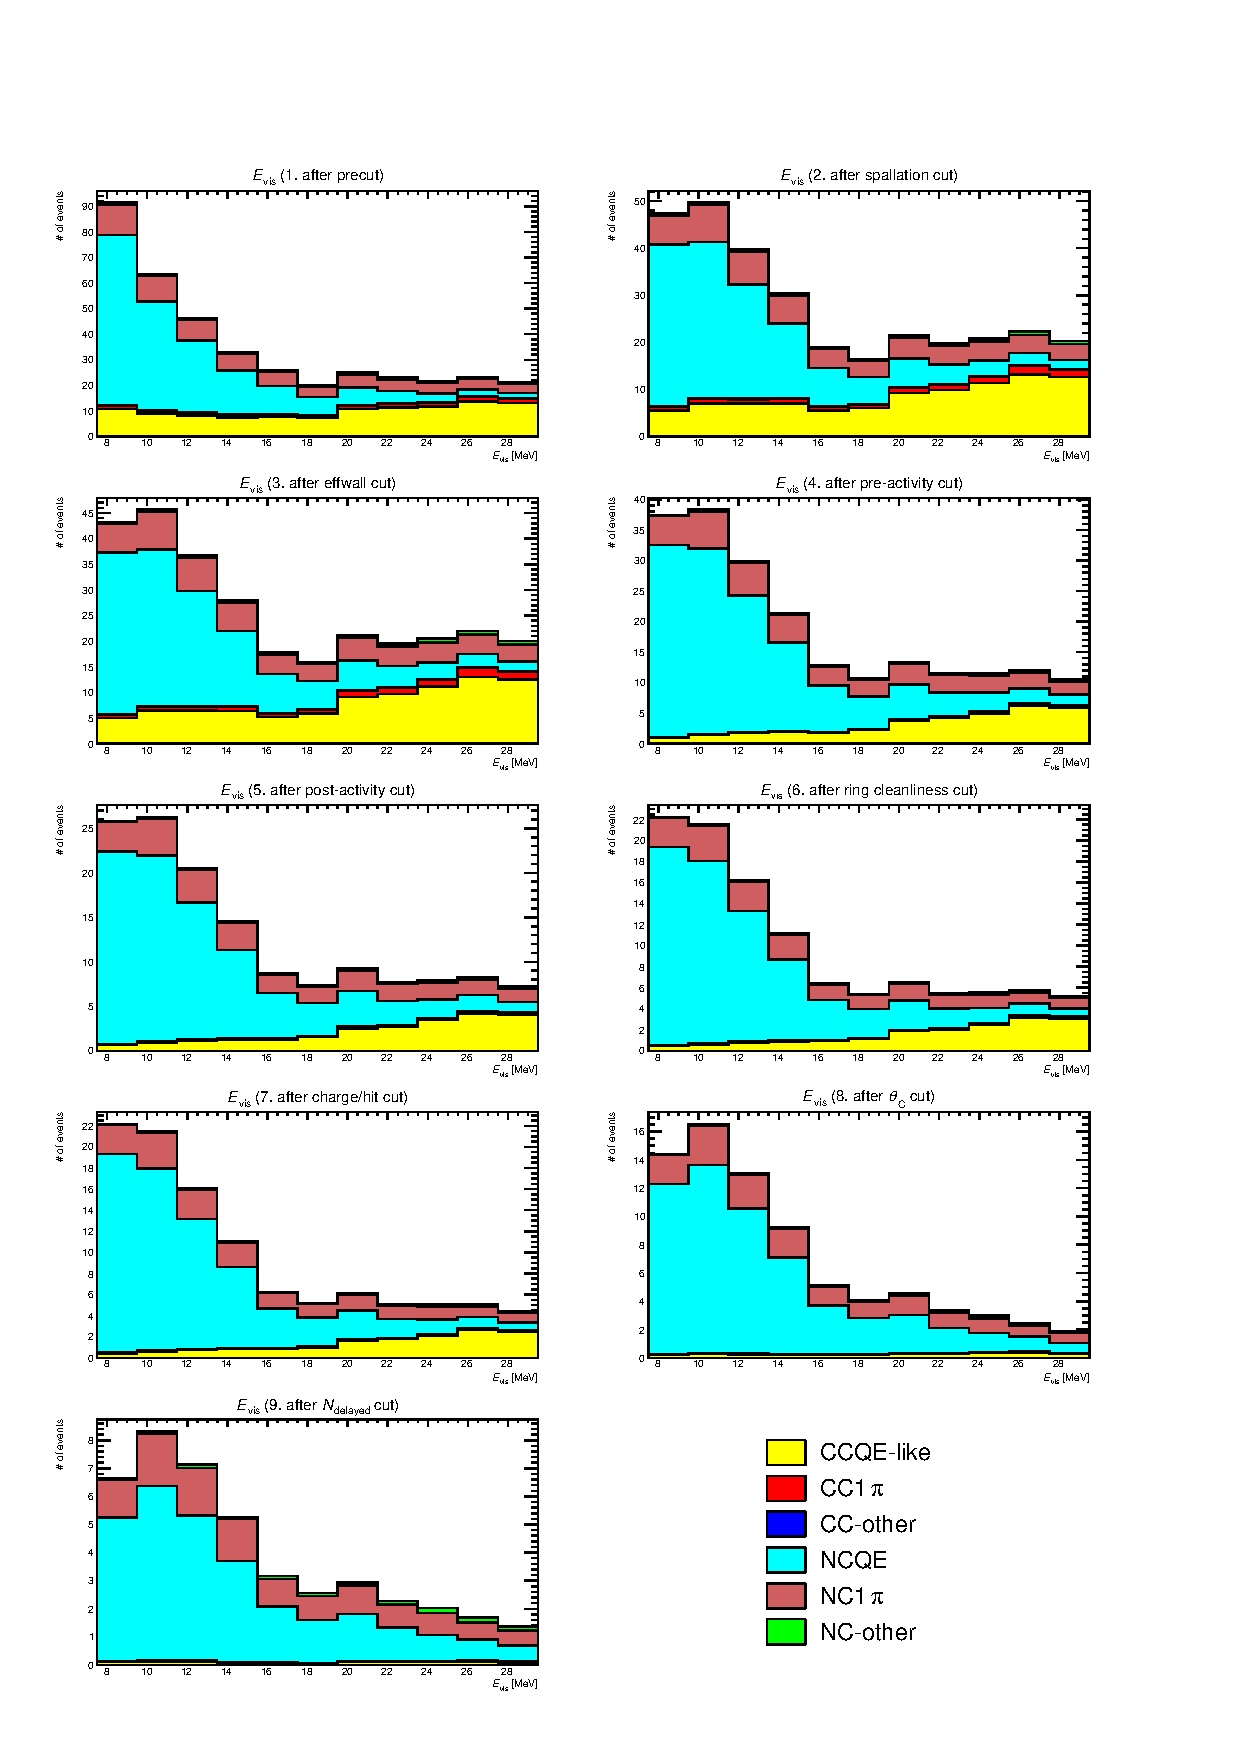
\includegraphics[width=15cm]{PDF/Dist_ATM/Che_50deg_tag_ge1/All/erec}
	\caption[$E_{\rm vis}$ for atmospheric neutrino events]{
	$E_{\rm vis}$ for atmospheric neutrino events.
	Event reductions are performed in the order shown in the title.
	}\label{ATM_erec}
\end{figure}

\begin{figure}[h]
	\centering
	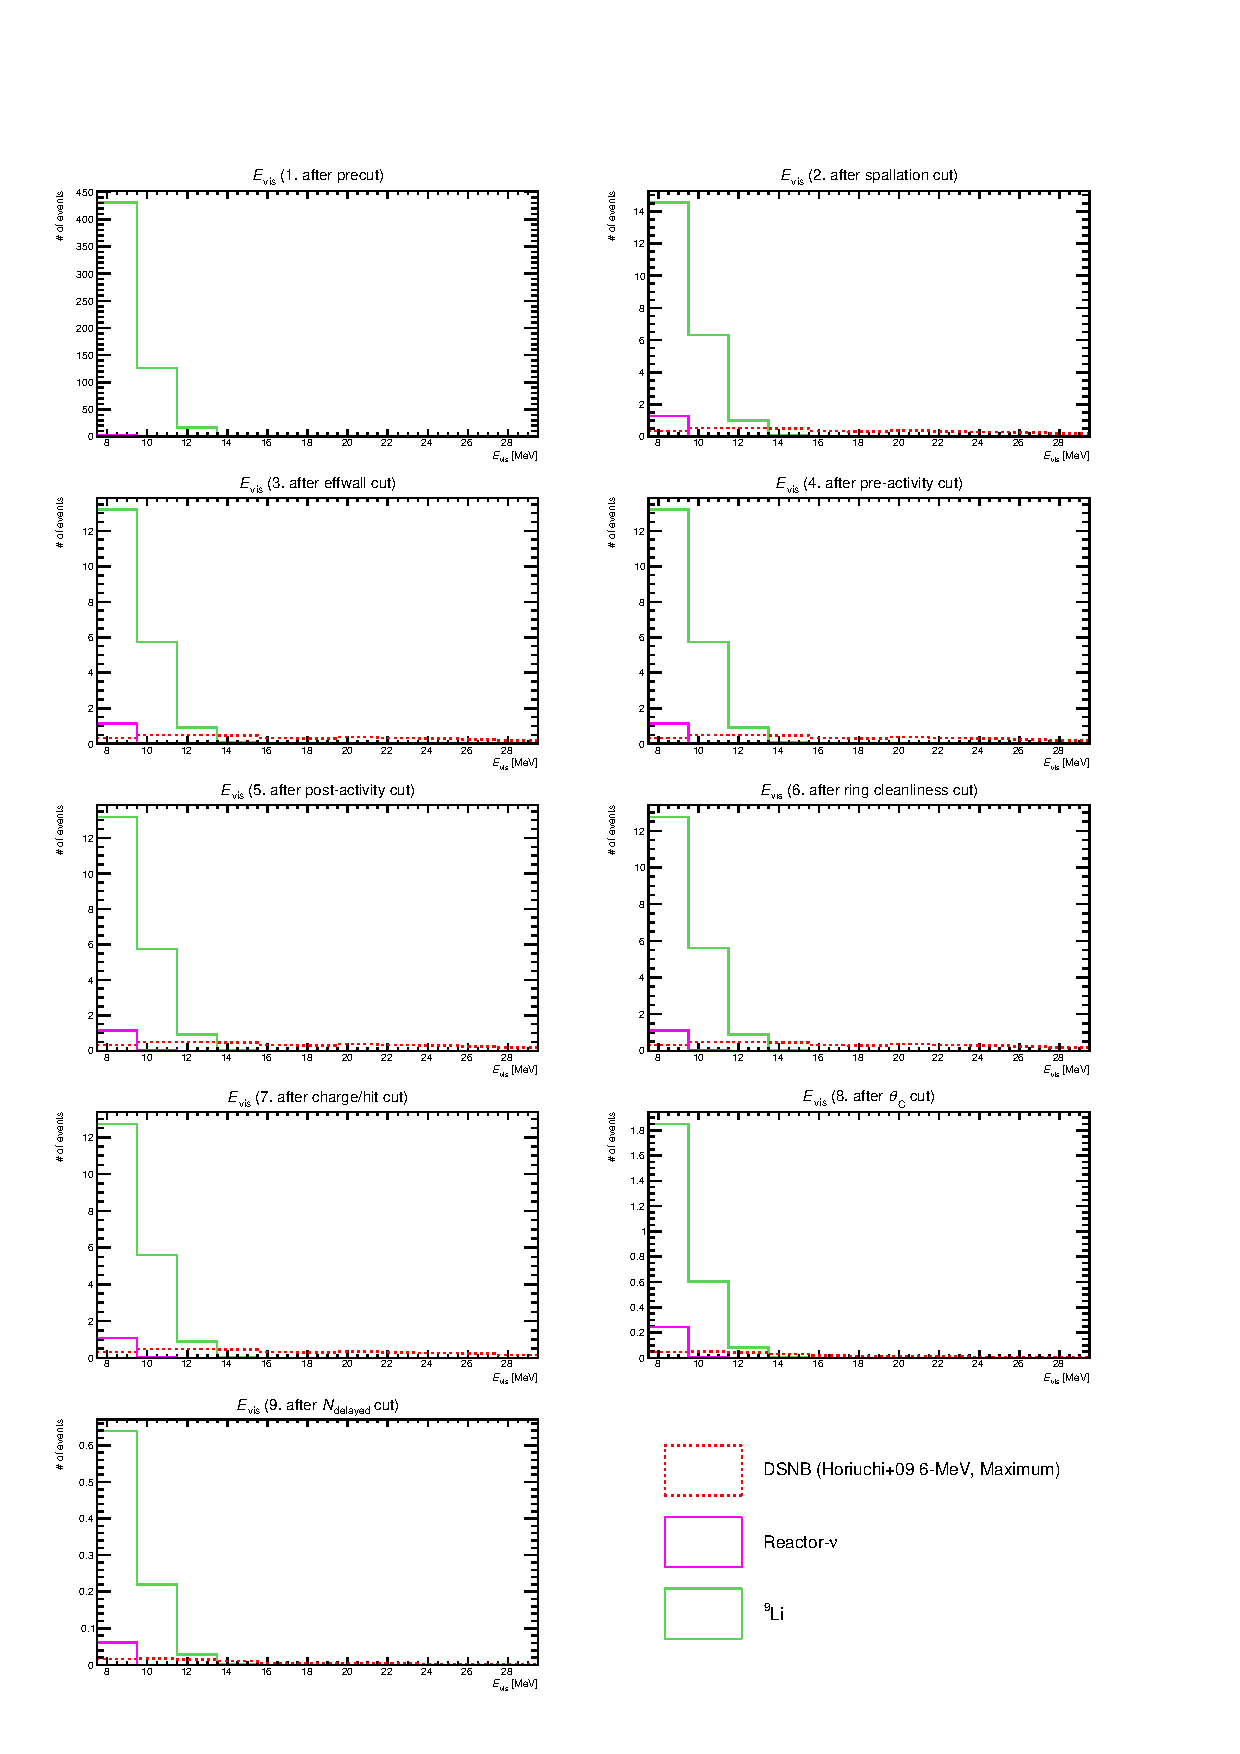
\includegraphics[width=15cm]{PDF/Dist_Nuebar/Che_50deg_tag_ge1/erec}
	\caption[$E_{\rm vis}$ for spallation, reactor neutrino, and DSNB events]{
	$E_{\rm vis}$ for spallation, reactor neutrino, and DSNB events.
	Event reductions are performed in the order shown in the title.
	}\label{Nuebar_erec}
\end{figure}

\begin{figure}[h]
	\centering
	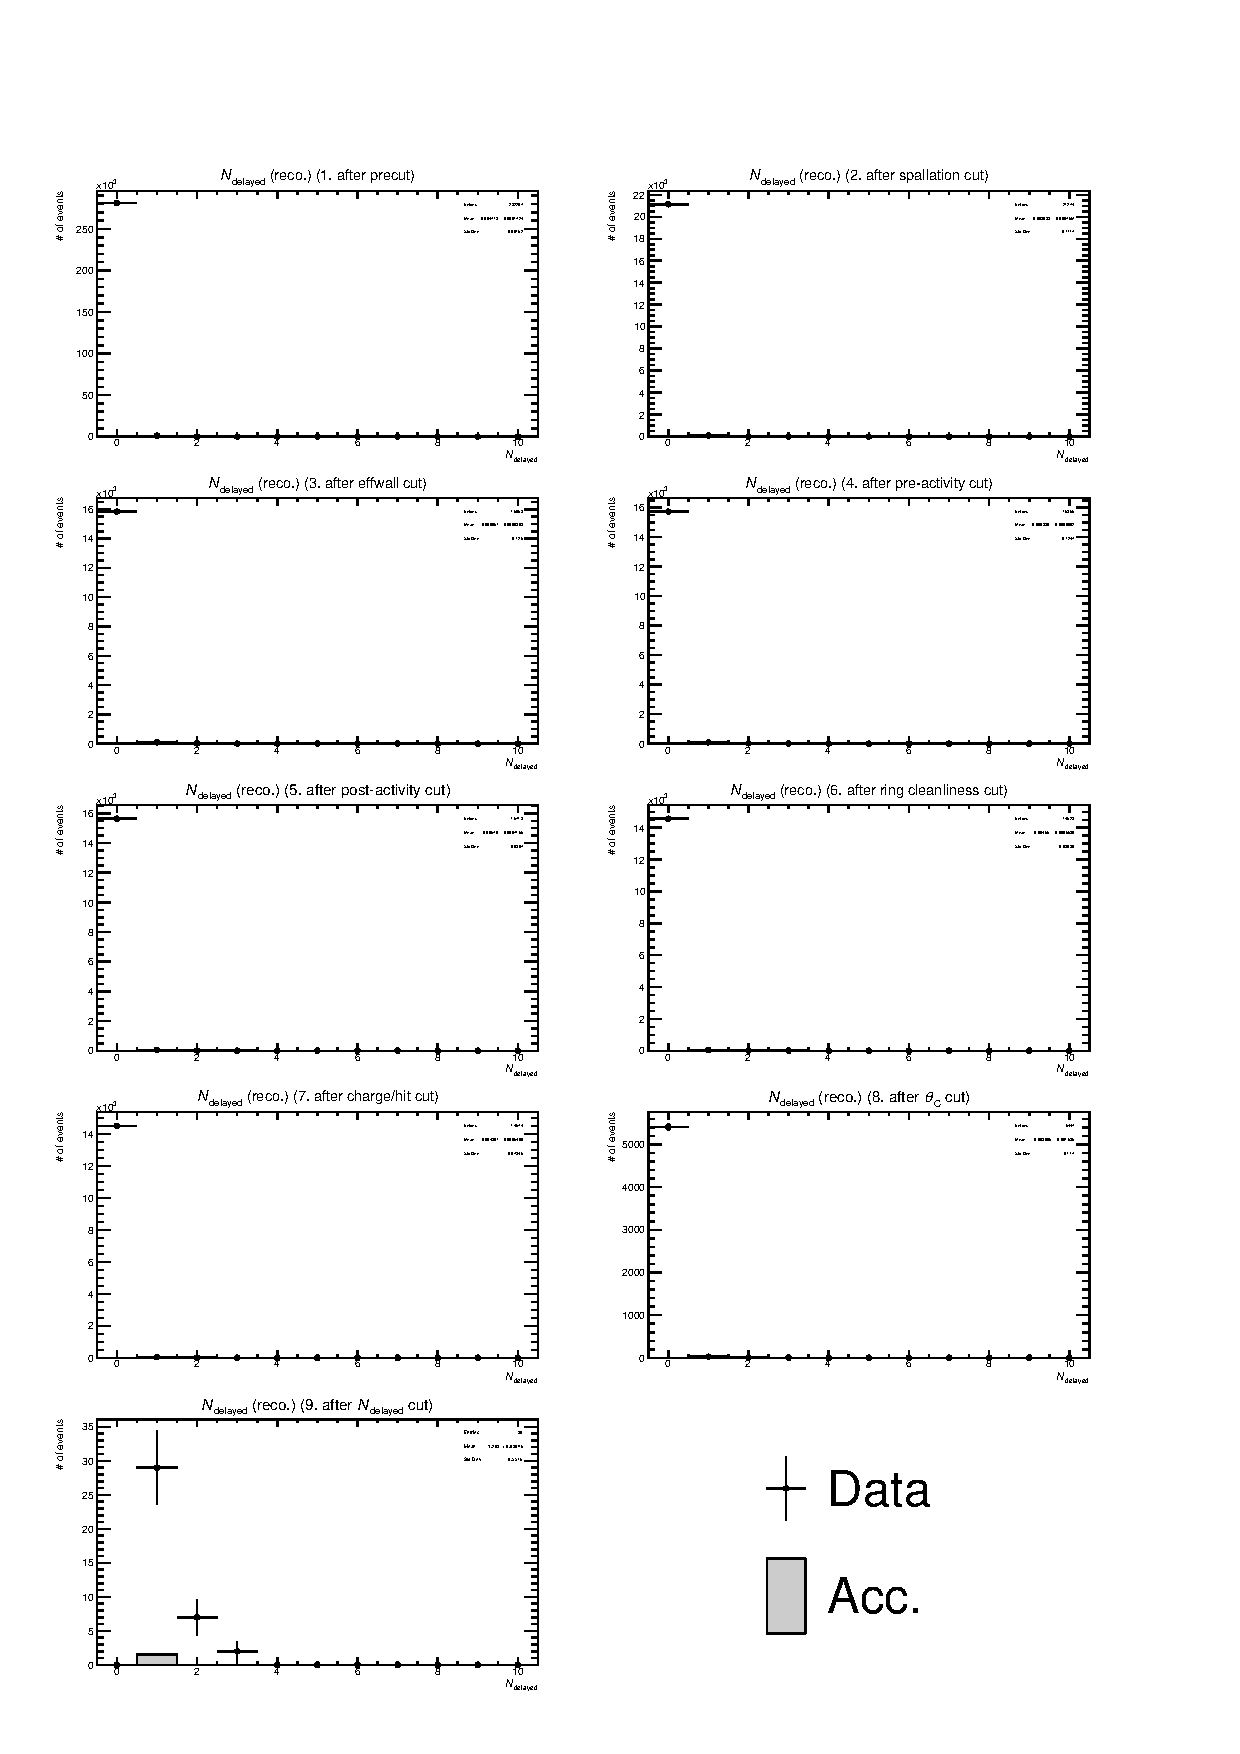
\includegraphics[width=15cm]{PDF/Dist_Data/Che_50deg_tag_ge1/RecoNumCap}
	\caption[$N_{\rm delayed}$ for the data and accidental coincidence events]{
	$N_{\rm delayed}$ for the data and accidental coincidence events.
	Event reductions are performed in the order shown in the title.
	}\label{Data_RecoNumCap}
\end{figure}

\begin{figure}[h]
	\centering
	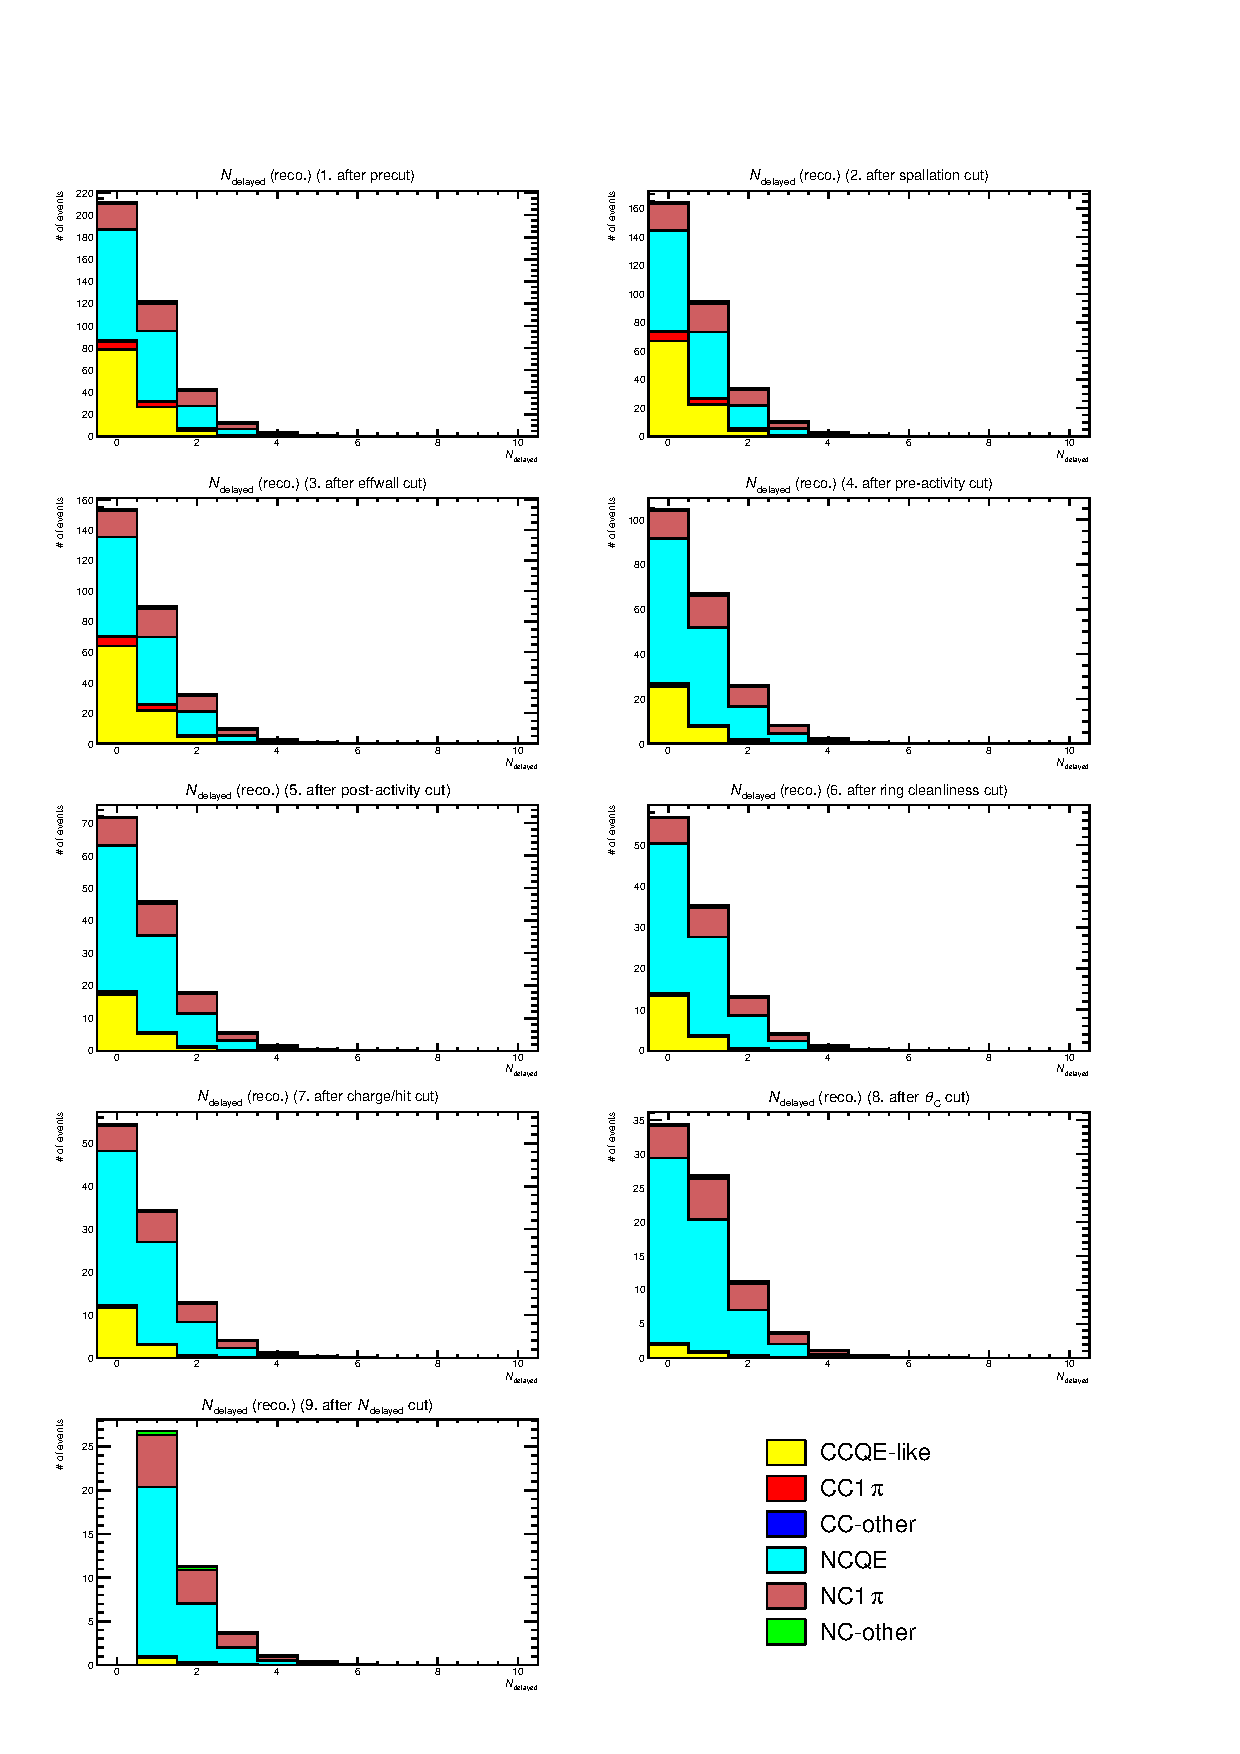
\includegraphics[width=15cm]{PDF/Dist_ATM/Che_50deg_tag_ge1/All/RecoNumCap}
	\caption[$N_{\rm delayed}$ for atmospheric neutrino events]{
	$N_{\rm delayed}$ for atmospheric neutrino events.
	Event reductions are performed in the order shown in the title.
	}\label{ATM_RecoNumCap}
\end{figure}

\begin{figure}[h]
	\centering
	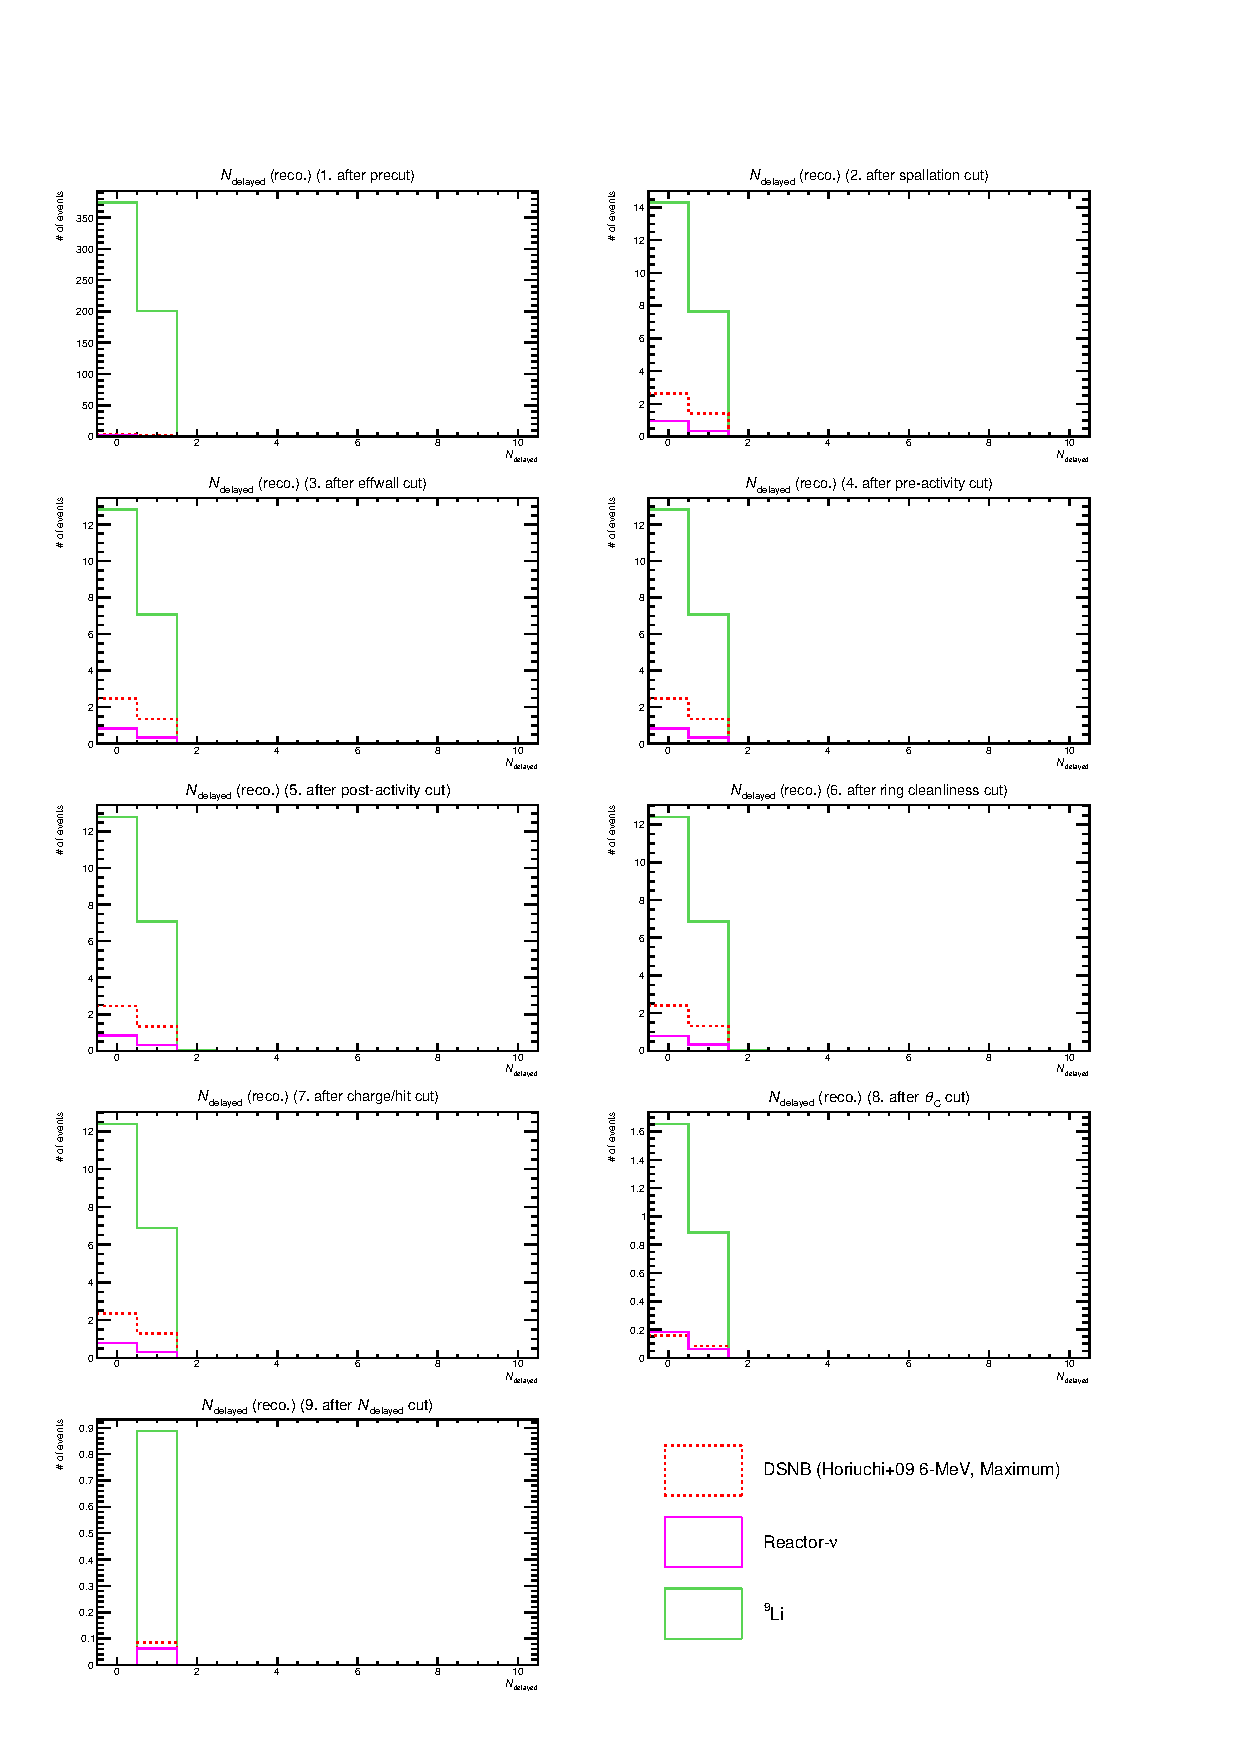
\includegraphics[width=15cm]{PDF/Dist_Nuebar/Che_50deg_tag_ge1/RecoNumCap}
	\caption[$N_{\rm delayed}$ for spallation, reactor neutrino, and DSNB events]{
	$N_{\rm delayed}$ for spallation, reactor neutrino, and DSNB events.
	Event reductions are performed in the order shown in the title.
	}\label{Nuebar_RecoNumCap}
\end{figure}

\begin{figure}[h]
	\centering
	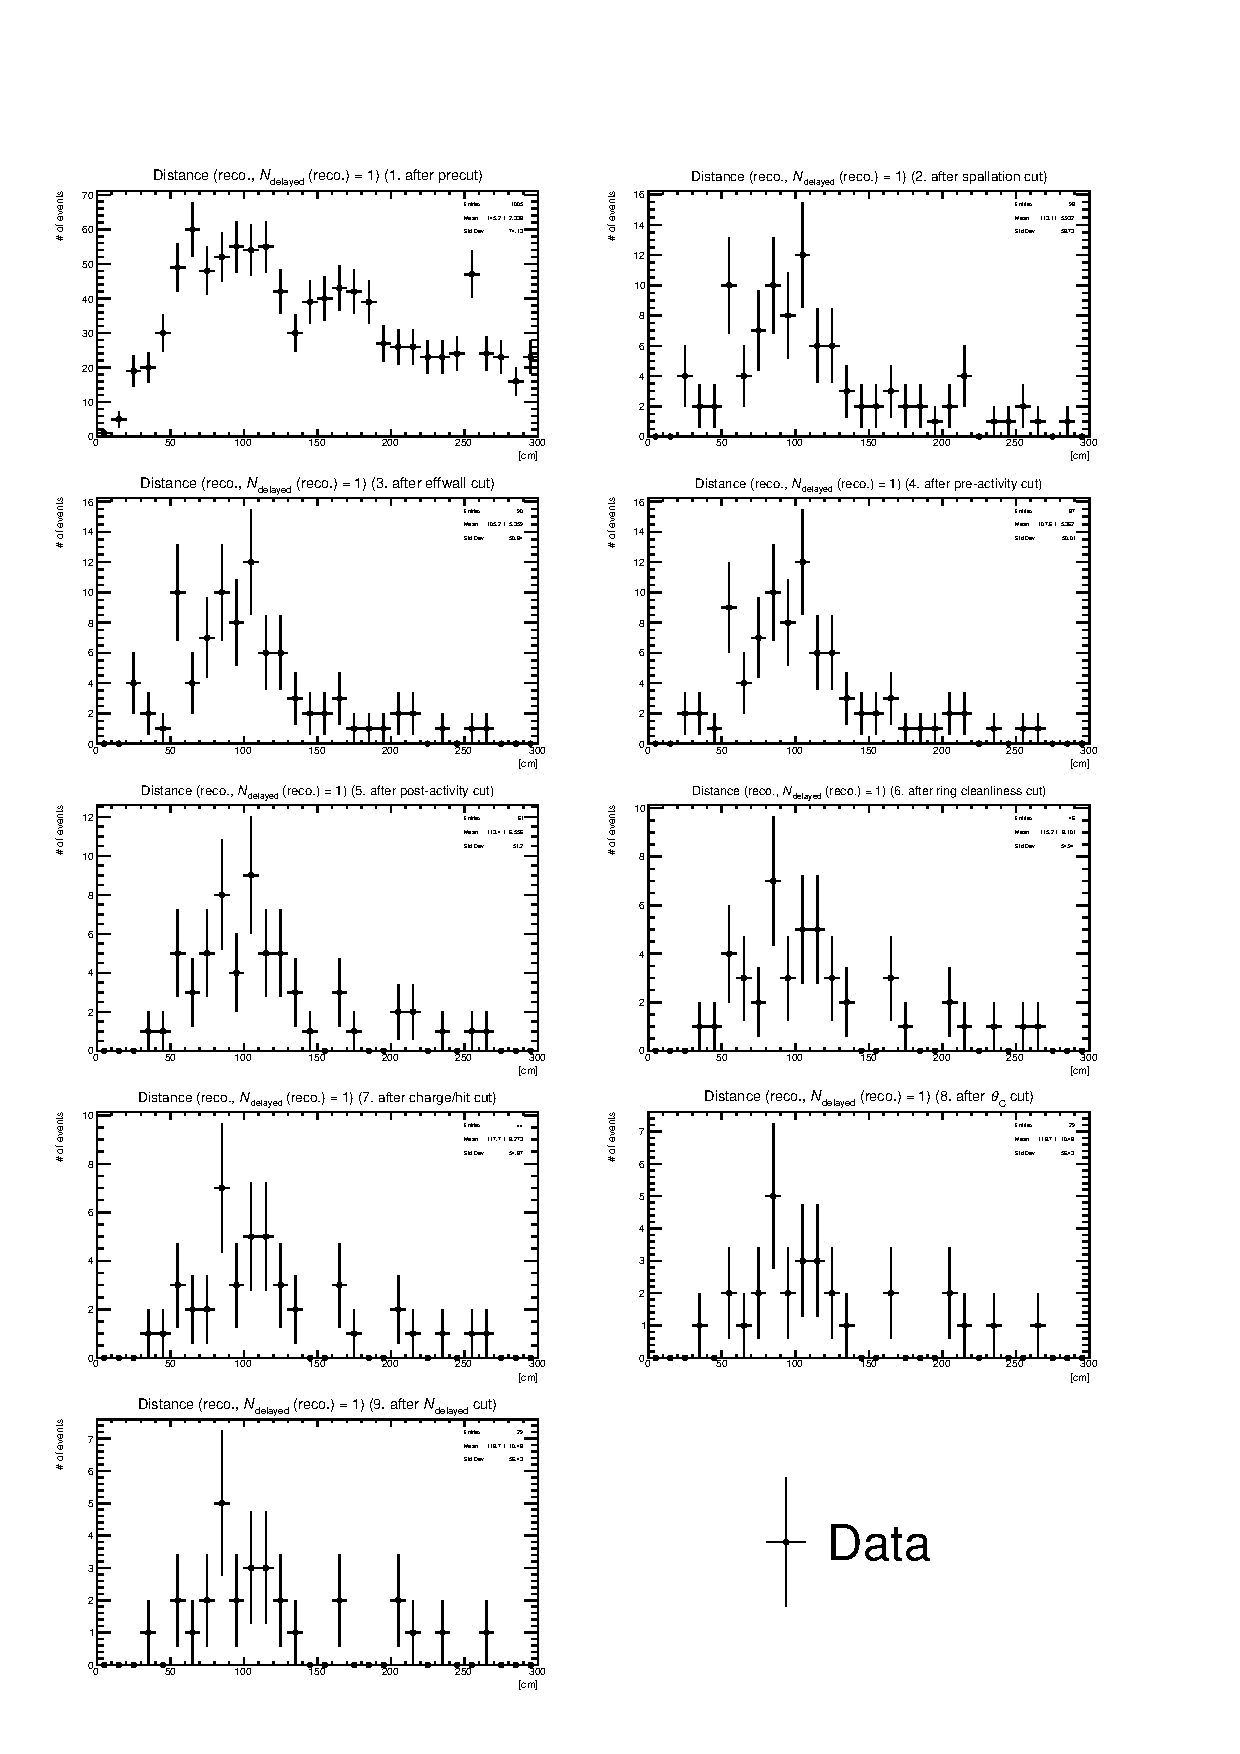
\includegraphics[width=15cm]{PDF/Dist_Data/Che_50deg_tag_ge1/RecoDisCap_1}
	\caption[Distance from prompt signal to delayed signal ($N_{\rm delayed}=1$) for the data and accidental coincidence events]{
	Distance from prompt signal to delayed signal ($N_{\rm delayed}=1$) for the data and accidental coincidence events.
	Event reductions are performed in the order shown in the title.
	}\label{Data_RecoDisCap_1}
\end{figure}

\begin{figure}[h]
	\centering
	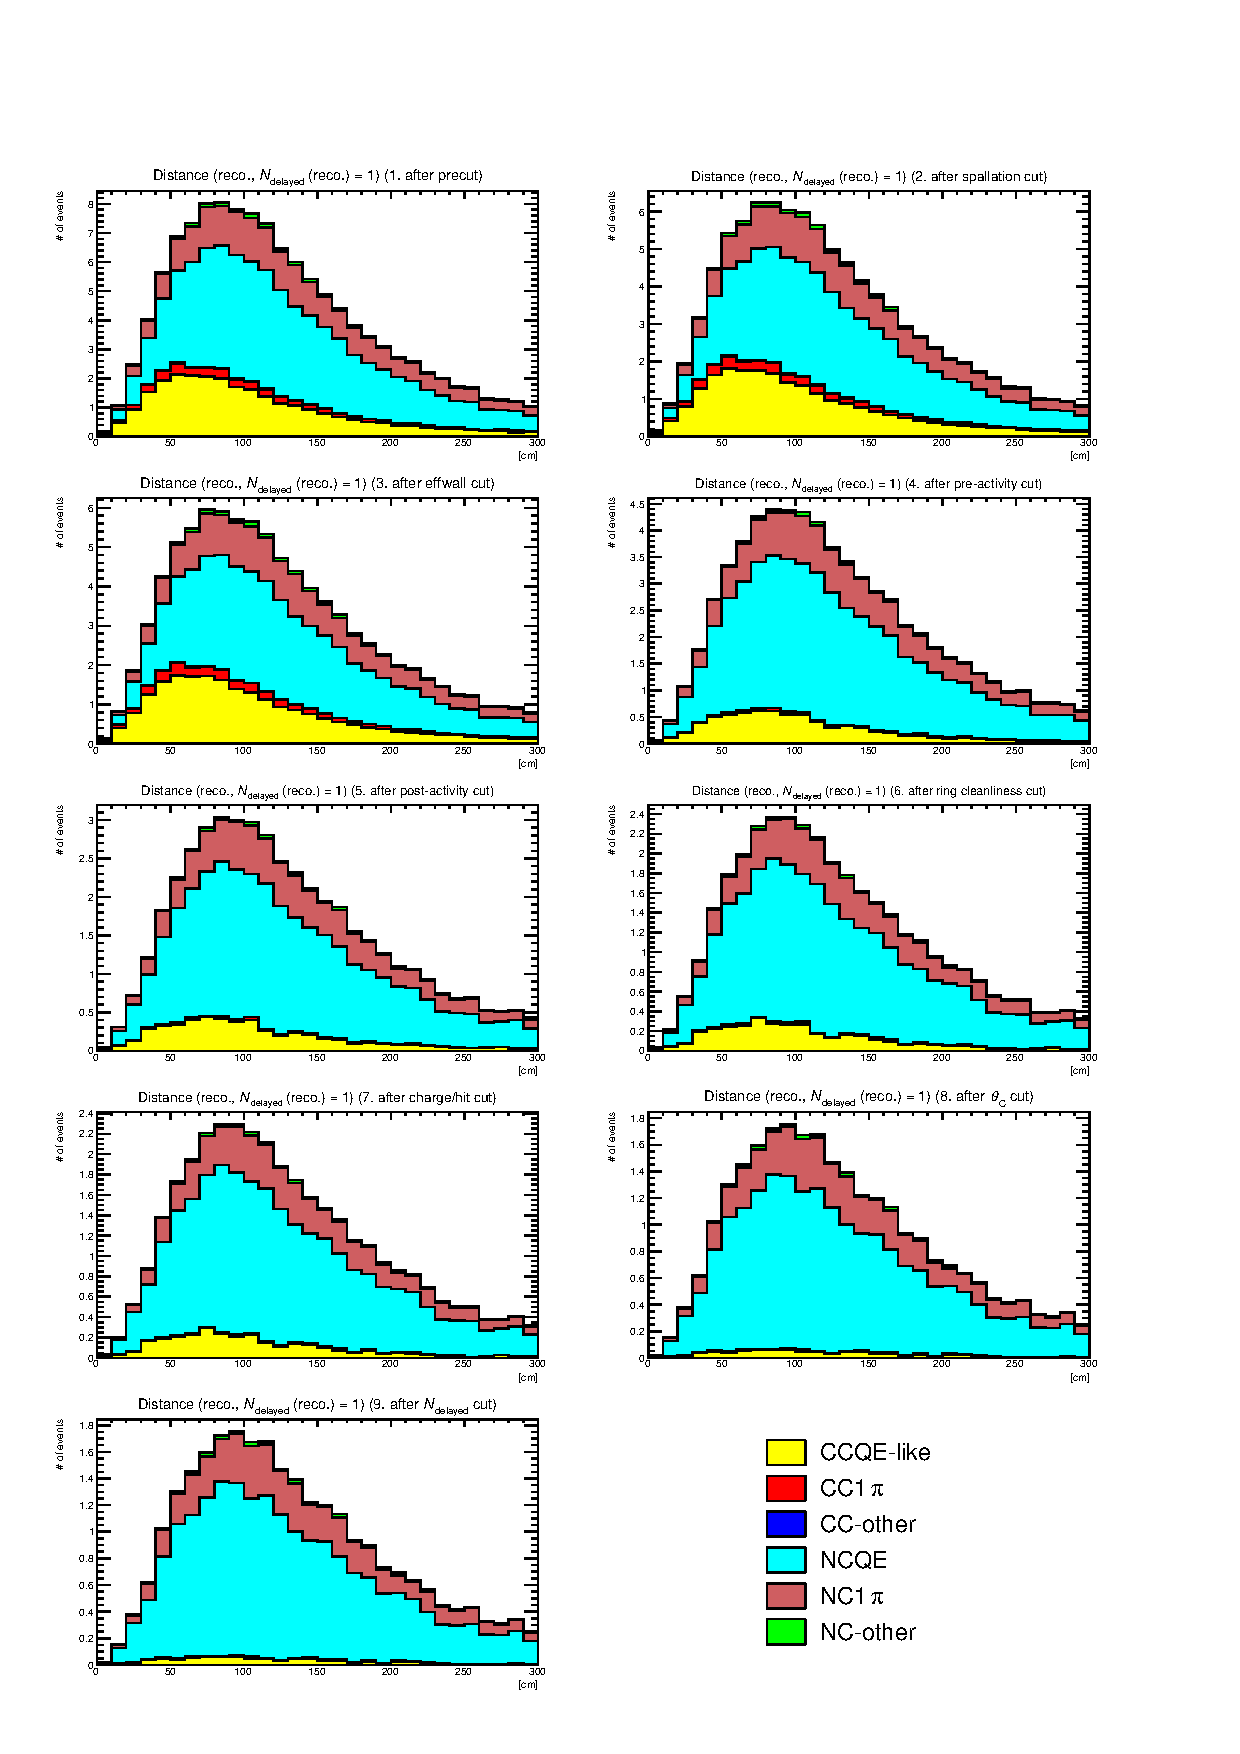
\includegraphics[width=15cm]{PDF/Dist_ATM/Che_50deg_tag_ge1/All/RecoDisCap_1}
	\caption[Distance from prompt signal to delayed signal ($N_{\rm delayed}=1$) for atmospheric neutrino events]{
	Distance from prompt signal to delayed signal ($N_{\rm delayed}=1$) for atmospheric neutrino events.
	Event reductions are performed in the order shown in the title.
	}\label{ATM_RecoDisCap_1}
\end{figure}

\begin{figure}[h]
	\centering
	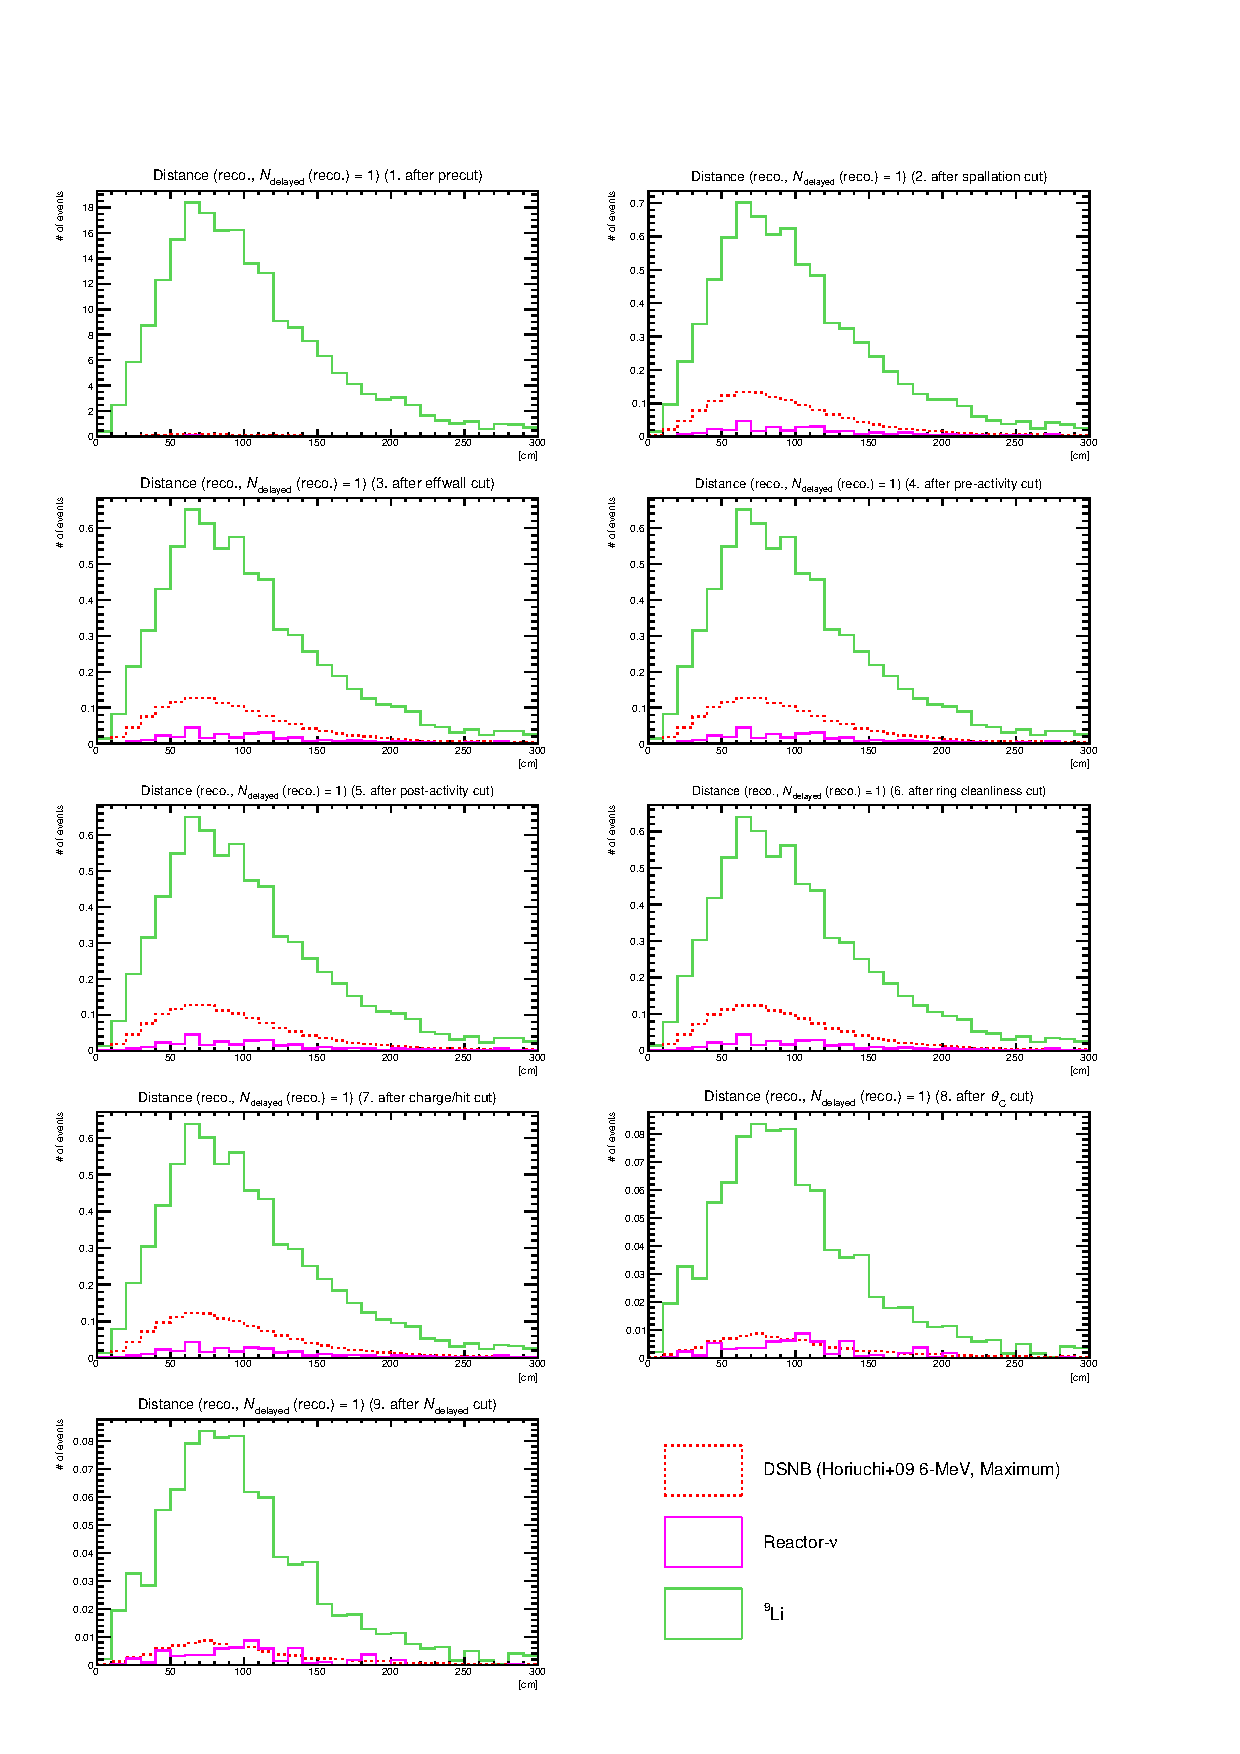
\includegraphics[width=15cm]{PDF/Dist_Nuebar/Che_50deg_tag_ge1/RecoDisCap_1}
	\caption[Distance from prompt signal to delayed signal ($N_{\rm delayed}=1$) for spallation, reactor neutrino, and DSNB events]{
	Distance from prompt signal to delayed signal ($N_{\rm delayed}=1$) for spallation, reactor neutrino, and DSNB events.
	Event reductions are performed in the order shown in the title.
	}\label{Nuebar_RecoDisCap_1}
\end{figure}





\clearpage
\subsection{Comparison of secondary interaction models}\label{App_Model}
\vs\hs
Other distributions and tables related to Section~\ref{Sec_Model} are summarized here.

\begin{figure}[H]
	\centering
	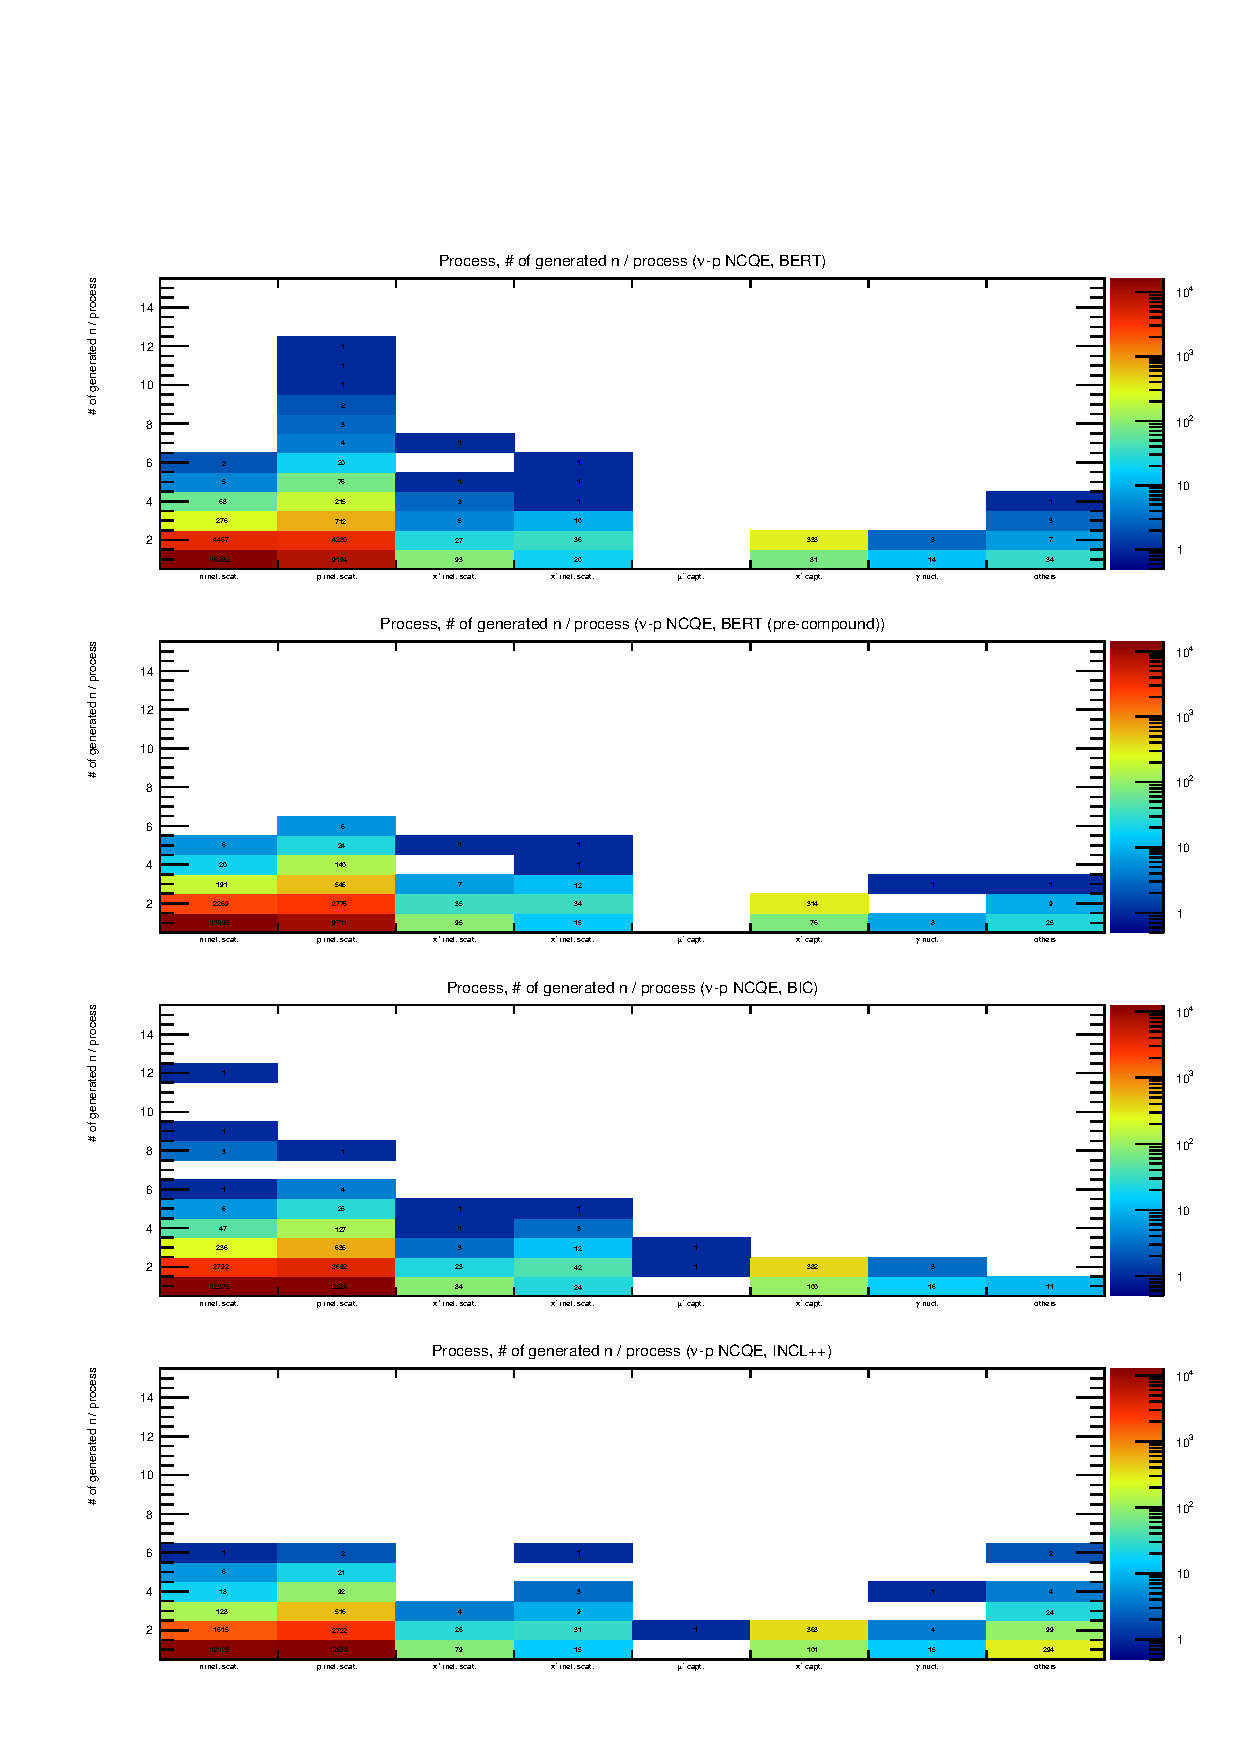
\includegraphics[width=15cm]{PDF/Secondary/Comparison_PreCompound/neutron/pdf2/Logz_Pro_NumSec_nuncqe_p}
	\caption[The number of generated neutrons per process after neutrino-proton NCQE reactions]{
	The number of generated neutrons per process after neutrino-proton NCQE reactions.
	Top, top middle, bottom middle, and bottom figure shows the case of BERT, BERT with the Geant4 pre-compound model, BIC, and INCL++, respectively.
	Horizontal axis shows processes that generated neutrons (neutron inelastic scattering, proton inelastic scattering, $\pi^{+}$ inelastic scattering, $\pi^{-}$ inelastic scattering, $\mu^{-}$ capture, $\pi^{-}$ capture, gamma-nuclear interaction, and others).
	}\label{Others_neutron_Logz_Pro_NumSec_nuncqe_p}
\end{figure}

\begin{figure}[h]
	\centering
	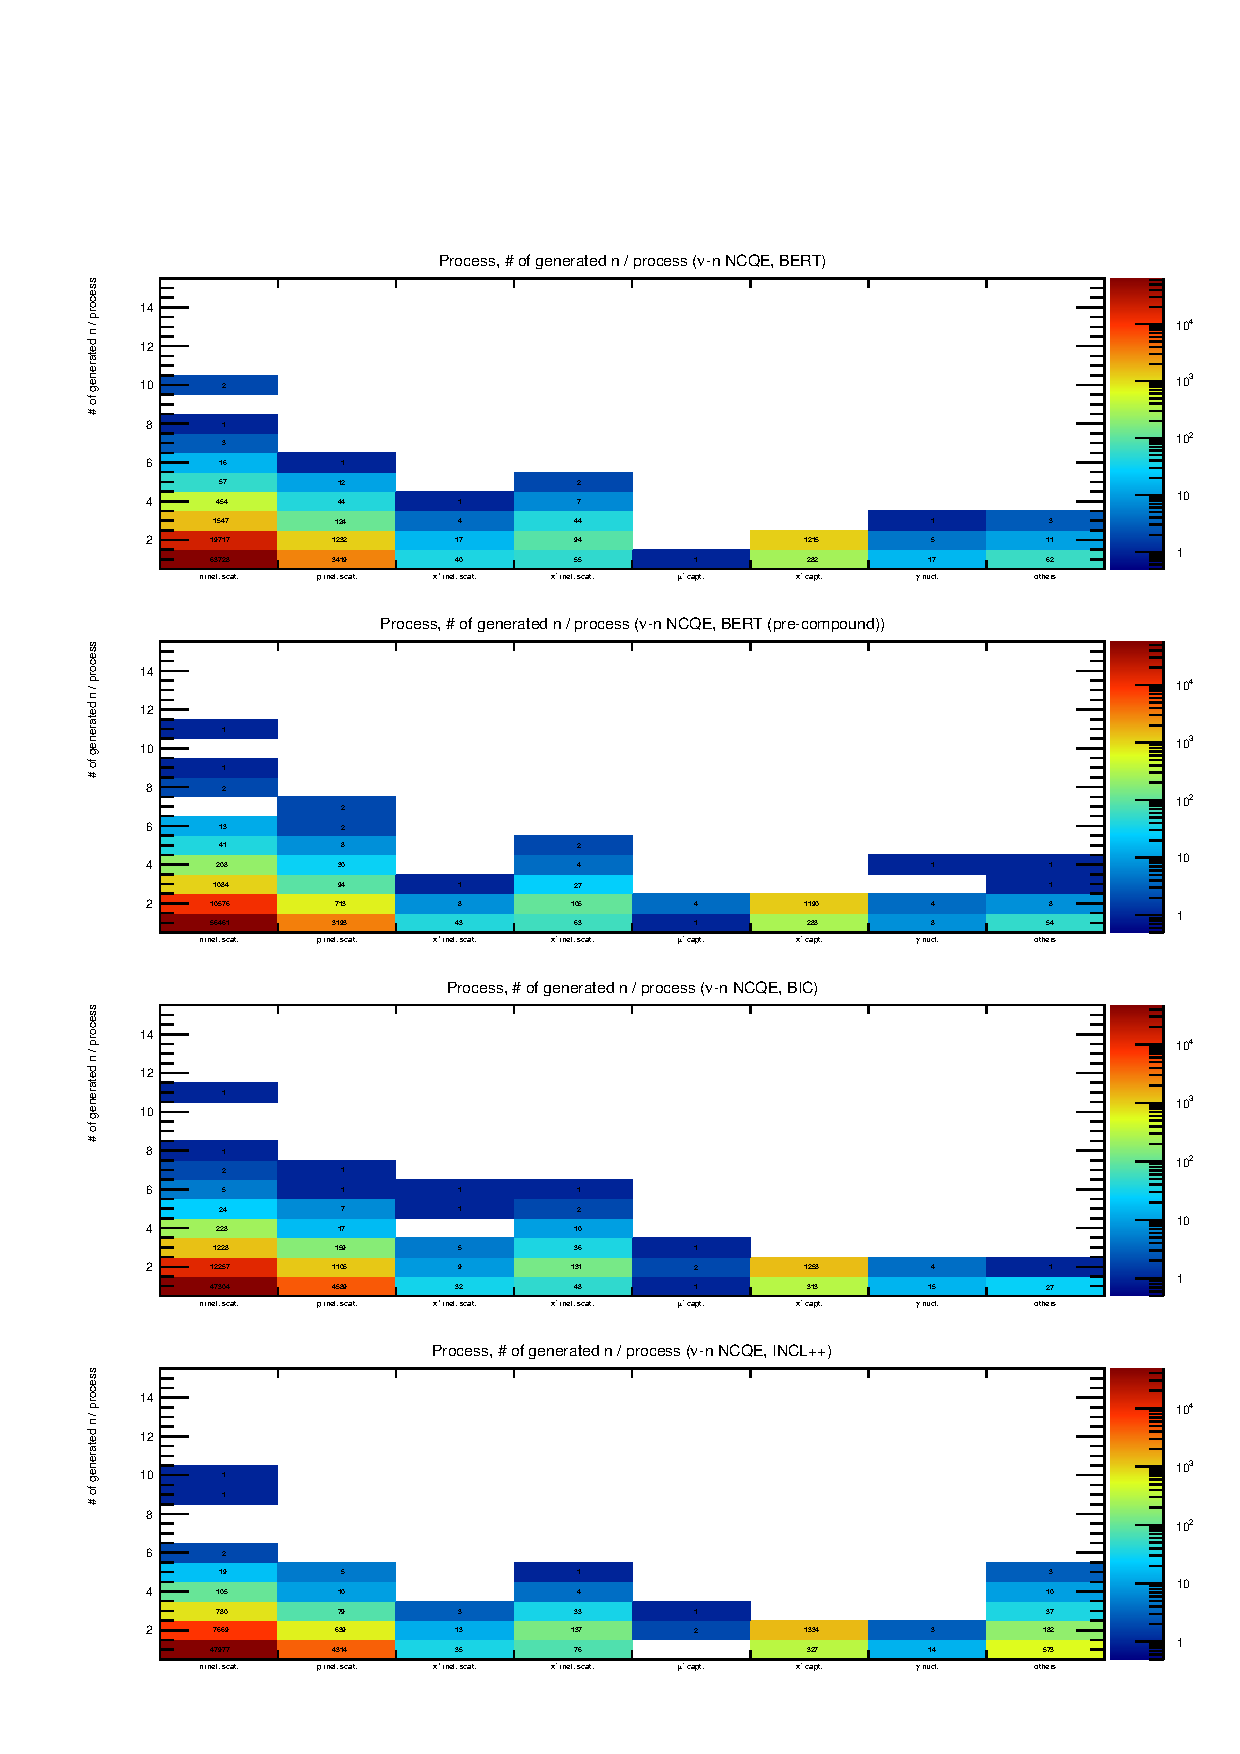
\includegraphics[width=15cm]{PDF/Secondary/Comparison_PreCompound/neutron/pdf2/Logz_Pro_NumSec_nuncqe_n}
	\caption[The number of generated neutrons per process after neutrino-neutron NCQE reactions]{
	The number of generated neutrons per process after neutrino-neutron NCQE reactions.
	Top, top middle, bottom middle, and bottom figure shows the case of BERT, BERT with the Geant4 pre-compound model, BIC, and INCL++, respectively.
	Horizontal axis shows processes that generated neutrons (neutron inelastic scattering, proton inelastic scattering, $\pi^{+}$ inelastic scattering, $\pi^{-}$ inelastic scattering, $\mu^{-}$ capture, $\pi^{-}$ capture, gamma-nuclear interaction, and others).
	}\label{Others_neutron_Logz_Pro_NumSec_nuncqe_n}
\end{figure}

\begin{figure}[h]
	\centering
	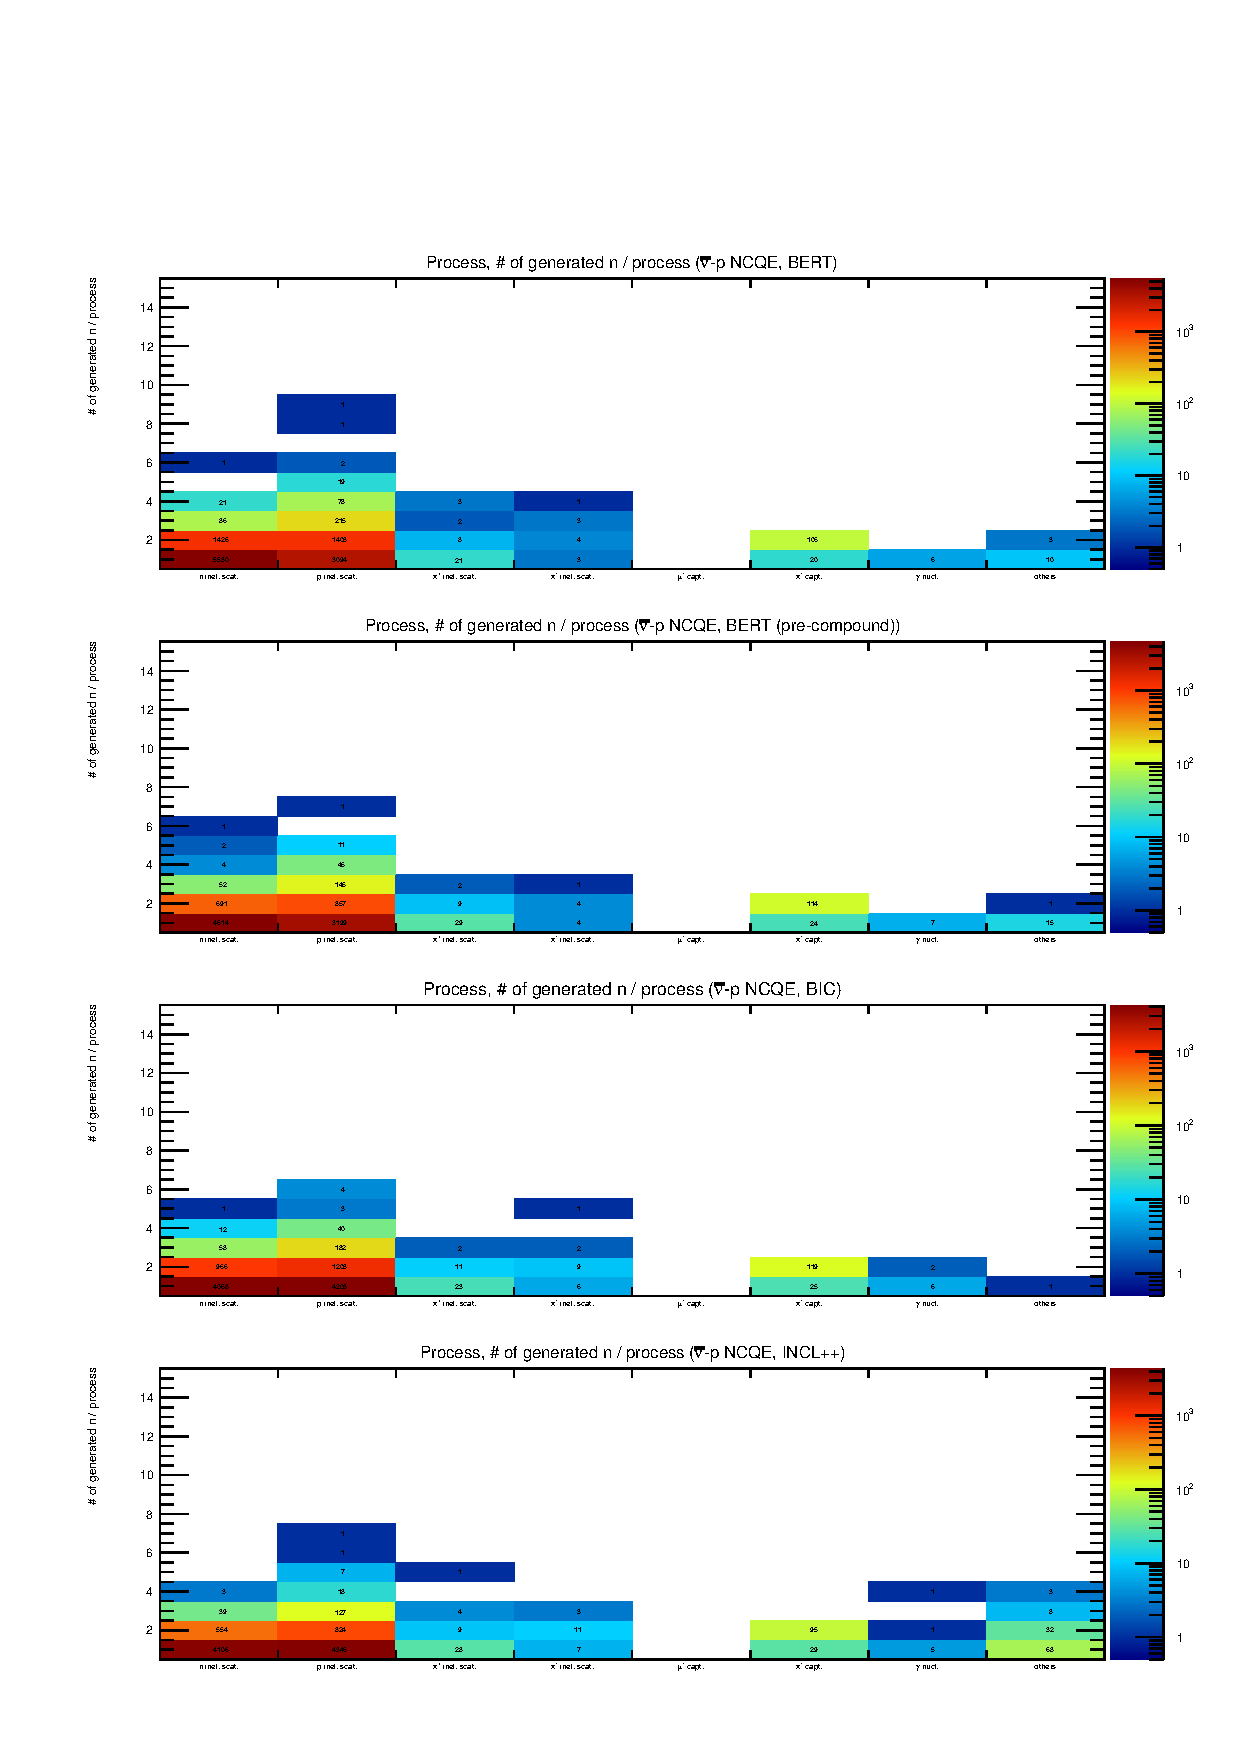
\includegraphics[width=15cm]{PDF/Secondary/Comparison_PreCompound/neutron/pdf2/Logz_Pro_NumSec_nubncqe_p}
	\caption[The number of generated neutrons per process after antineutrino-proton NCQE reactions]{
	The number of generated neutrons per process after antineutrino-proton NCQE reactions.
	Top, top middle, bottom middle, and bottom figure shows the case of BERT, BERT with the Geant4 pre-compound model, BIC, and INCL++, respectively.
	Horizontal axis shows processes that generated neutrons (neutron inelastic scattering, proton inelastic scattering, $\pi^{+}$ inelastic scattering, $\pi^{-}$ inelastic scattering, $\mu^{-}$ capture, $\pi^{-}$ capture, gamma-nuclear interaction, and others).
	}\label{Others_neutron_Logz_Pro_NumSec_nubncqe_p}
\end{figure}

\begin{figure}[h]
	\centering
	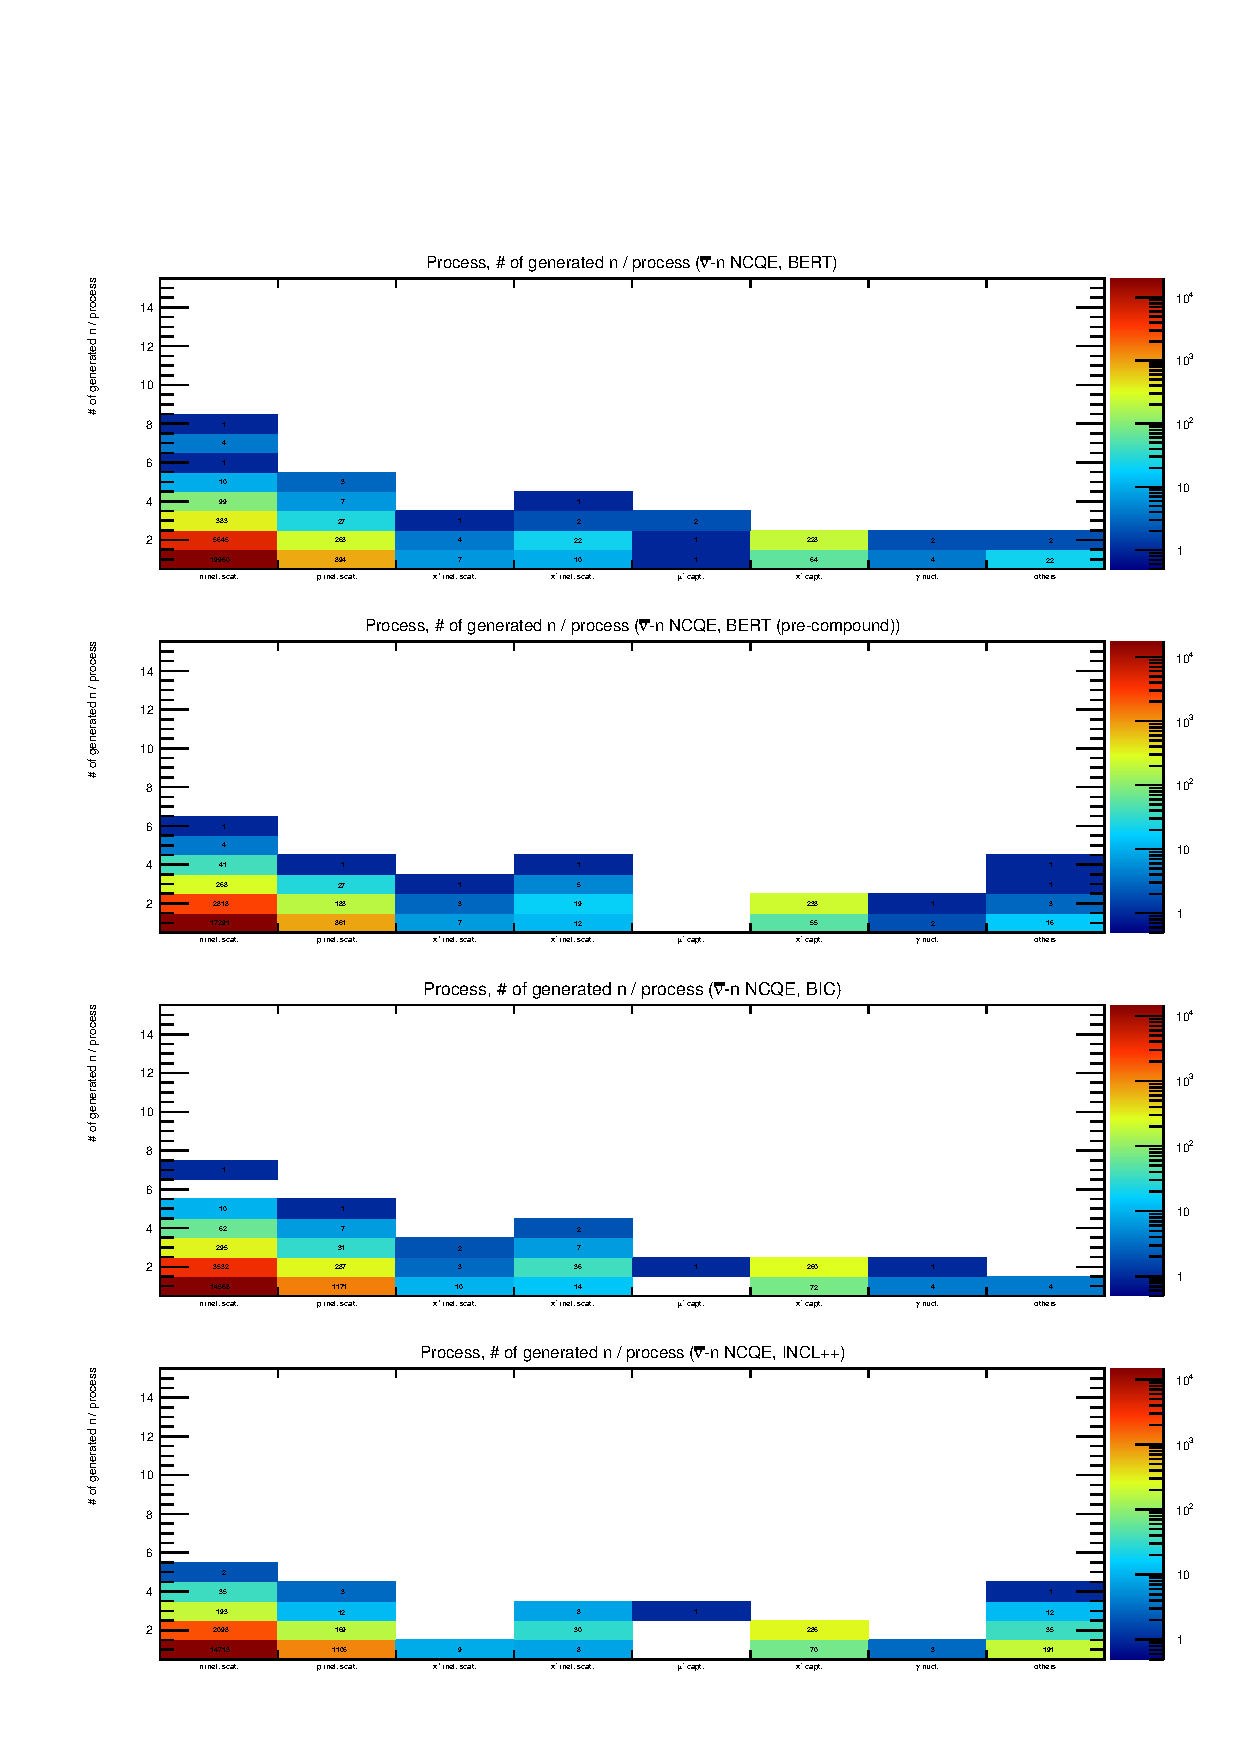
\includegraphics[width=15cm]{PDF/Secondary/Comparison_PreCompound/neutron/pdf2/Logz_Pro_NumSec_nubncqe_n}
	\caption[The number of generated neutrons per process after antineutrino-neutron NCQE reactions]{
	The number of generated neutrons per process after antineutrino-neutron NCQE reactions.
	Top, top middle, bottom middle, and bottom figure shows the case of BERT, BERT with the Geant4 pre-compound model, BIC, and INCL++, respectively.
	Horizontal axis shows processes that generated neutrons (neutron inelastic scattering, proton inelastic scattering, $\pi^{+}$ inelastic scattering, $\pi^{-}$ inelastic scattering, $\mu^{-}$ capture, $\pi^{-}$ capture, gamma-nuclear interaction, and others).
	}\label{Others_neutron_Logz_Pro_NumSec_nubncqe_n}
\end{figure}

\begin{figure}[h]
	\centering
	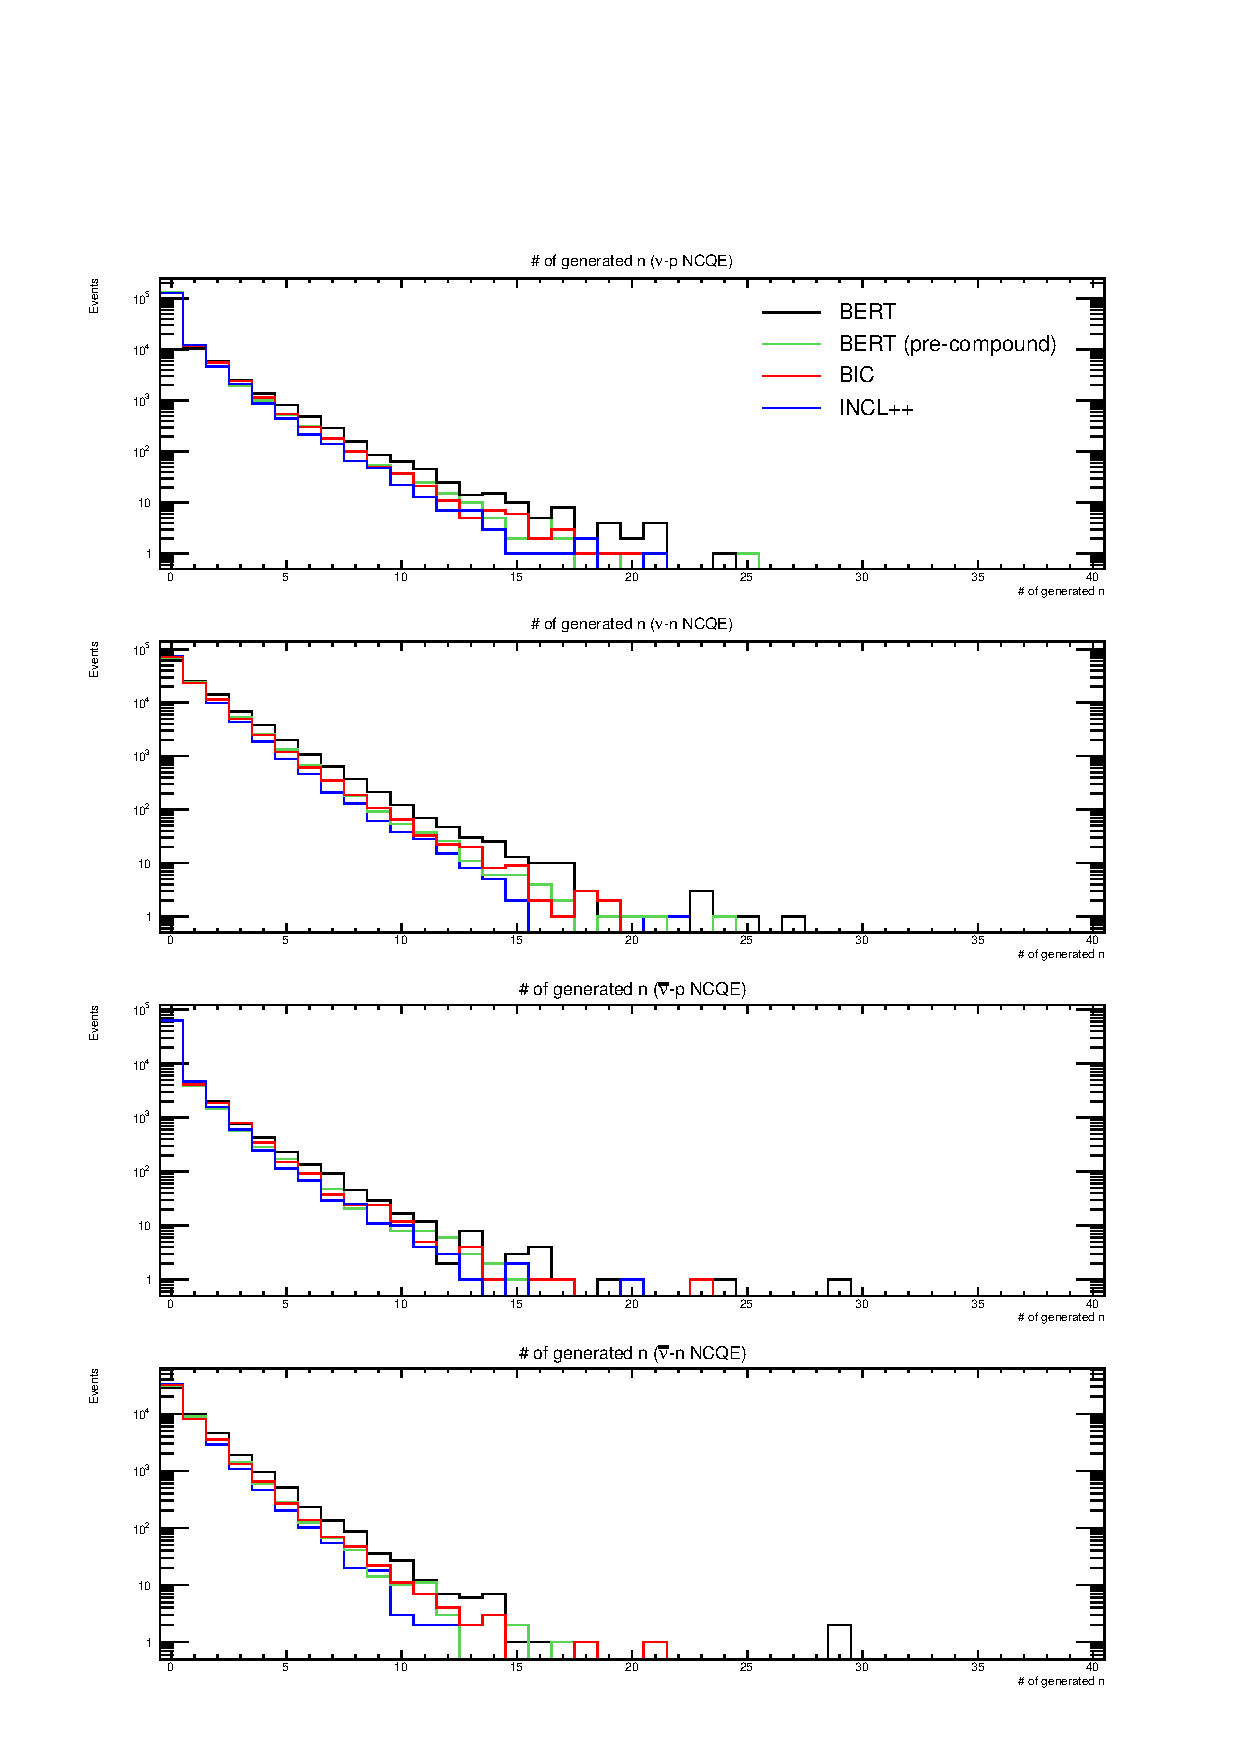
\includegraphics[width=16cm]{PDF/Secondary/Comparison_PreCompound/neutron/pdf1/Logy_NumSec}
	\caption[The number of neutrons generated after NCQE reactions]{
	The number of neutrons generated after NCQE reactions.
	Top, top middle, bottom middle, and bottom figure shows the case of neutrino-proton, neutrino-neutron, antineutrino-proton, and antineutrino-neutron NCQE reactions, respectively.
	Black, green, red, and blue line shows the case of BERT, BERT with the Geant4 pre-compound model, BIC, and INCL++, respectively.
	}\label{Others_neutron_Logy_NumSec}
\end{figure}

\begin{figure}[h]
	\centering
	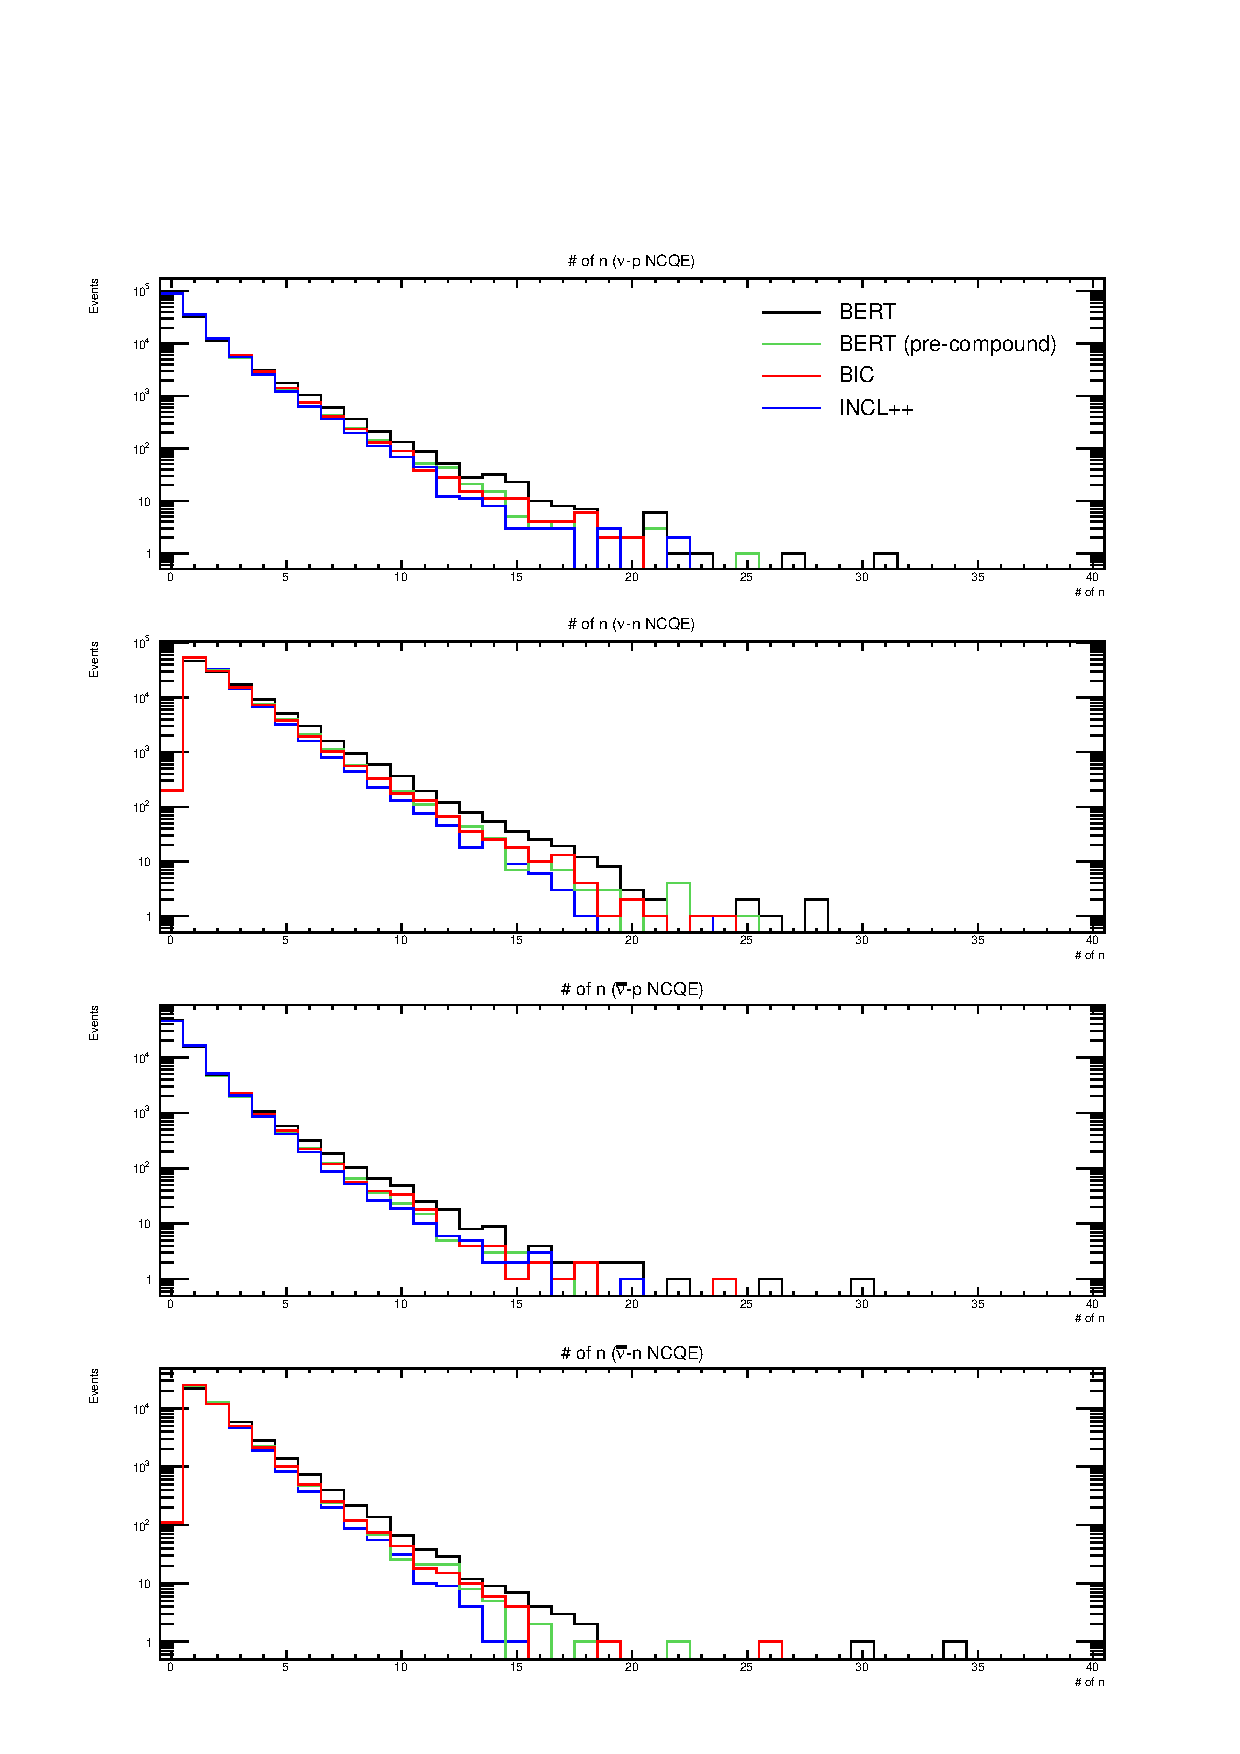
\includegraphics[width=16cm]{PDF/Secondary/Comparison_PreCompound/neutron/pdf1/Logy_Num}
	\caption[The total number of neutrons]{
	The total number of neutrons.
	Top, top middle, bottom middle, and bottom figure shows the case of neutrino-proton, neutrino-neutron, antineutrino-proton, and antineutrino-neutron NCQE reactions, respectively.
	Black, green, red, and blue line shows the case of BERT, BERT with the Geant4 pre-compound model, BIC, and INCL++, respectively.
	}\label{Others_neutron_Logy_Num}
\end{figure}

\begin{figure}[h]
	\centering
	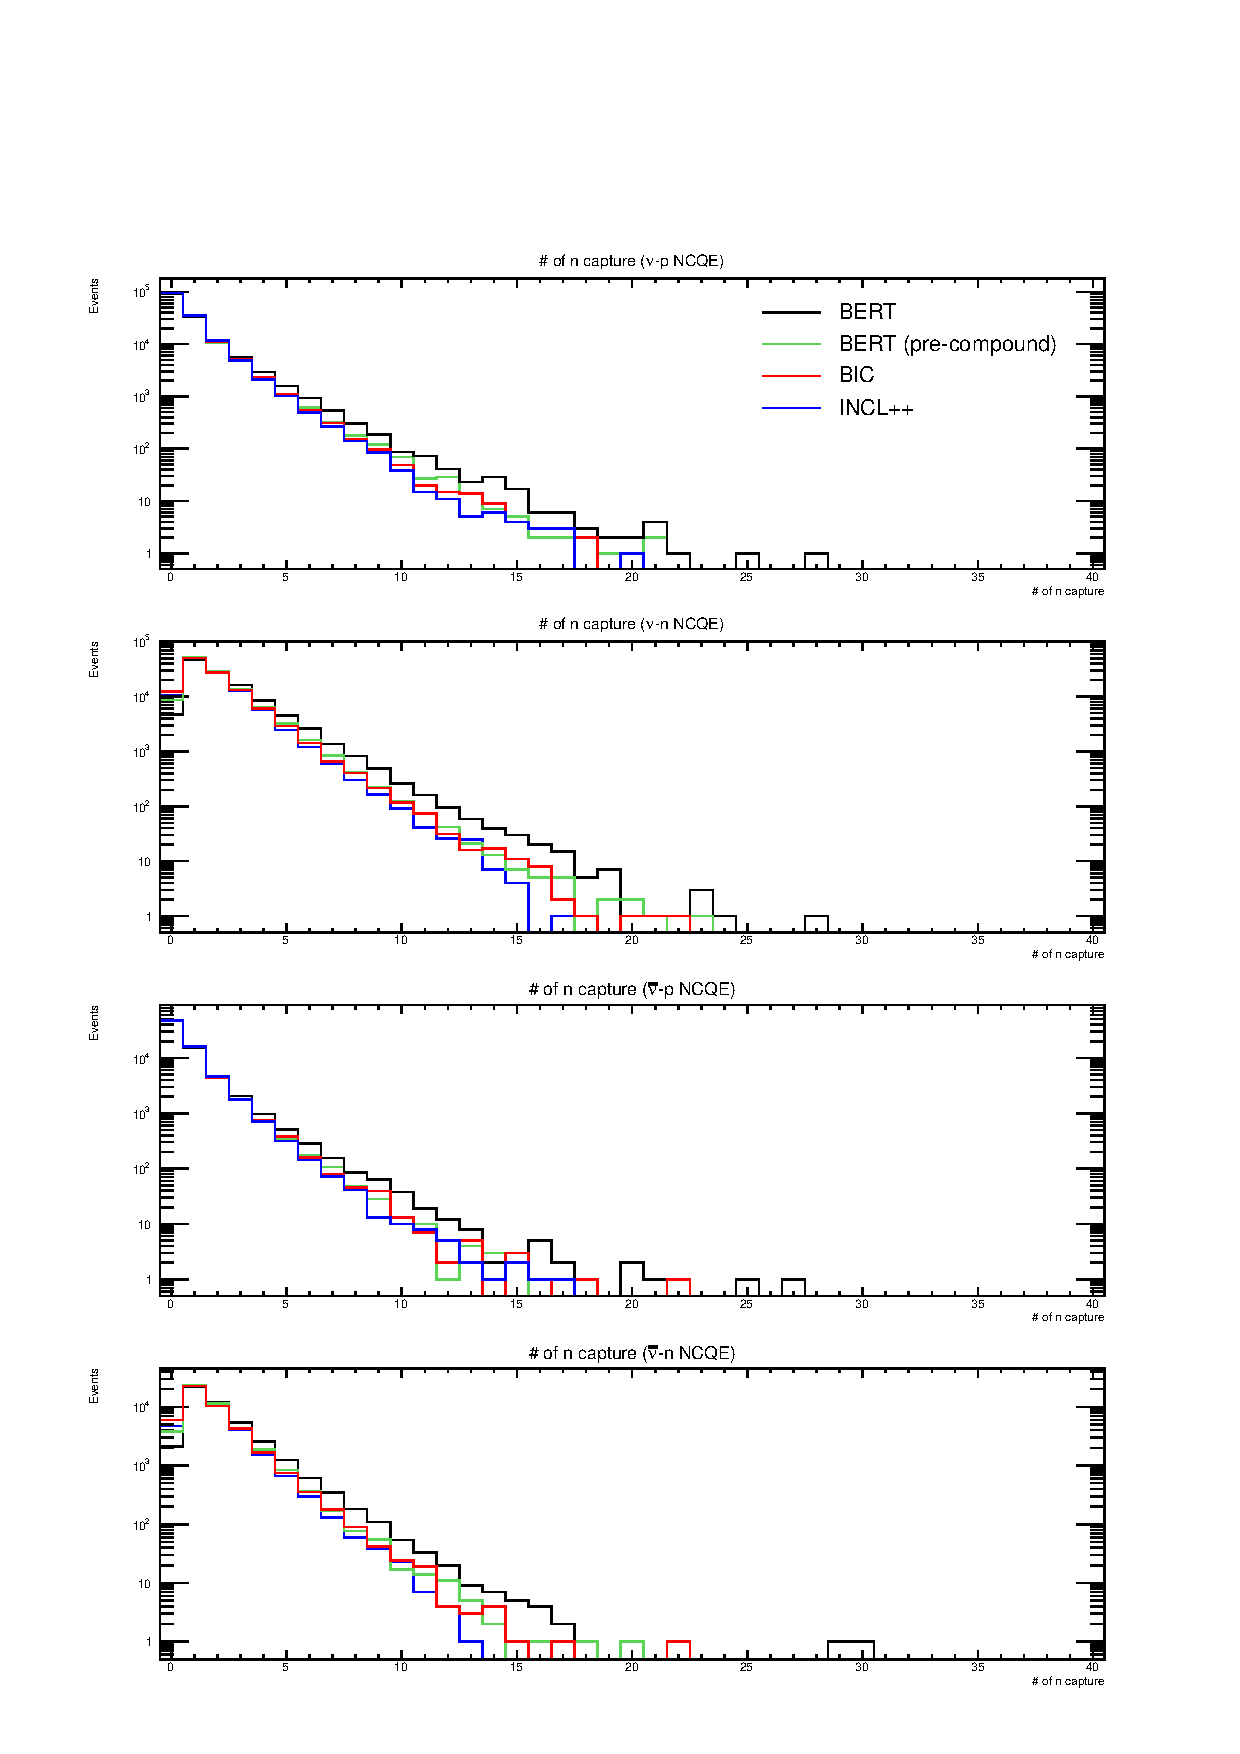
\includegraphics[width=16cm]{PDF/Secondary/Comparison_PreCompound/neutron/pdf1/Logy_NumCap}
	\caption[The number of neutron captures]{
	The number of neutron captures.
	Top, top middle, bottom middle, and bottom figure shows the case of neutrino-proton, neutrino-neutron, antineutrino-proton, and antineutrino-neutron NCQE reactions, respectively.
	Black, green, red, and blue line shows the case of BERT, BERT with the Geant4 pre-compound model, BIC, and INCL++, respectively.
	}\label{Others_neutron_Logy_NumCap}
\end{figure}

\begin{figure}[h]
	\centering
	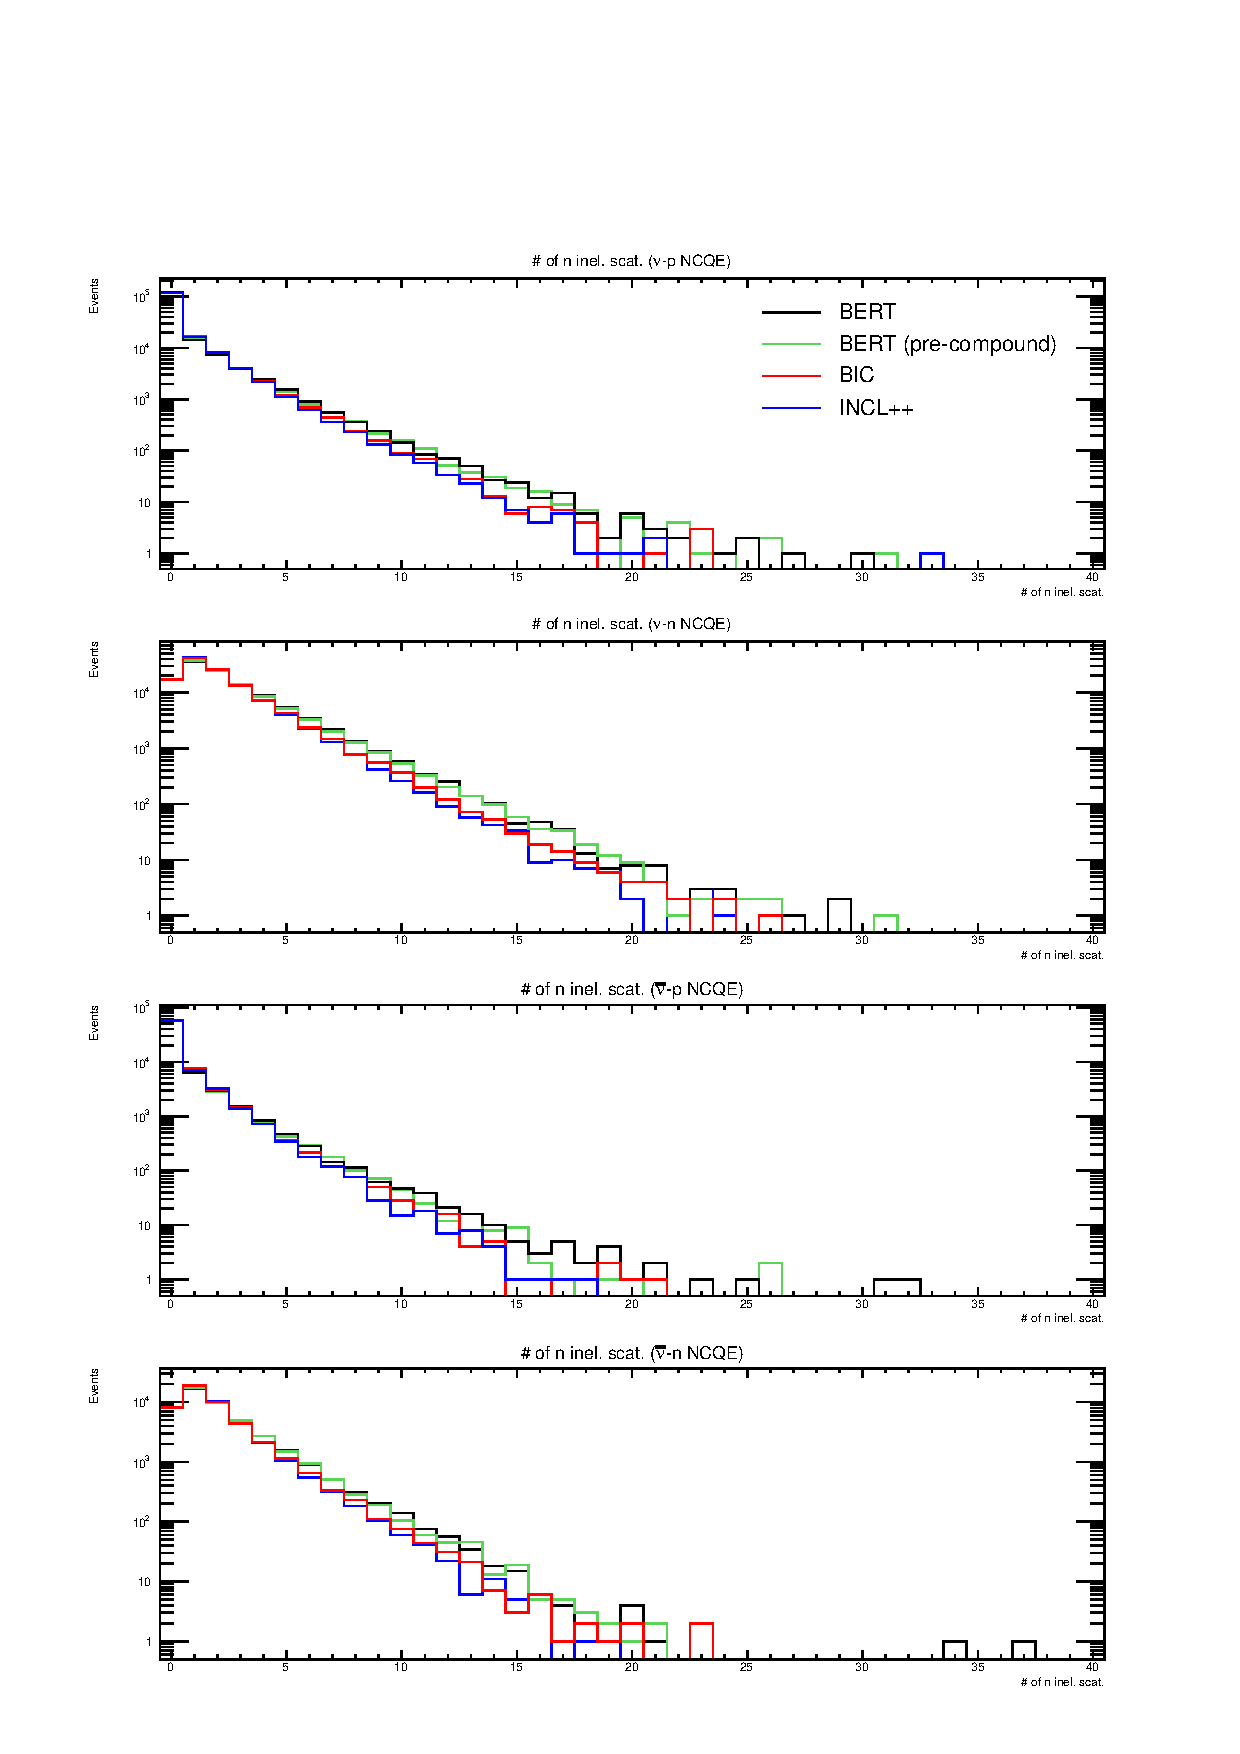
\includegraphics[width=16cm]{PDF/Secondary/Comparison_PreCompound/neutron/pdf1/Logy_NumIne}
	\caption[The number of neutron inelastic scattering reactions]{
	The number of neutron inelastic scattering reactions.
	Top, top middle, bottom middle, and bottom figure shows the case of neutrino-proton, neutrino-neutron, antineutrino-proton, and antineutrino-neutron NCQE reactions, respectively.
	Black, green, red, and blue line shows the case of BERT, BERT with the Geant4 pre-compound model, BIC, and INCL++, respectively.
	}\label{Others_neutron_Logy_NumIne}
\end{figure}

\begin{figure}[h]
	\centering
	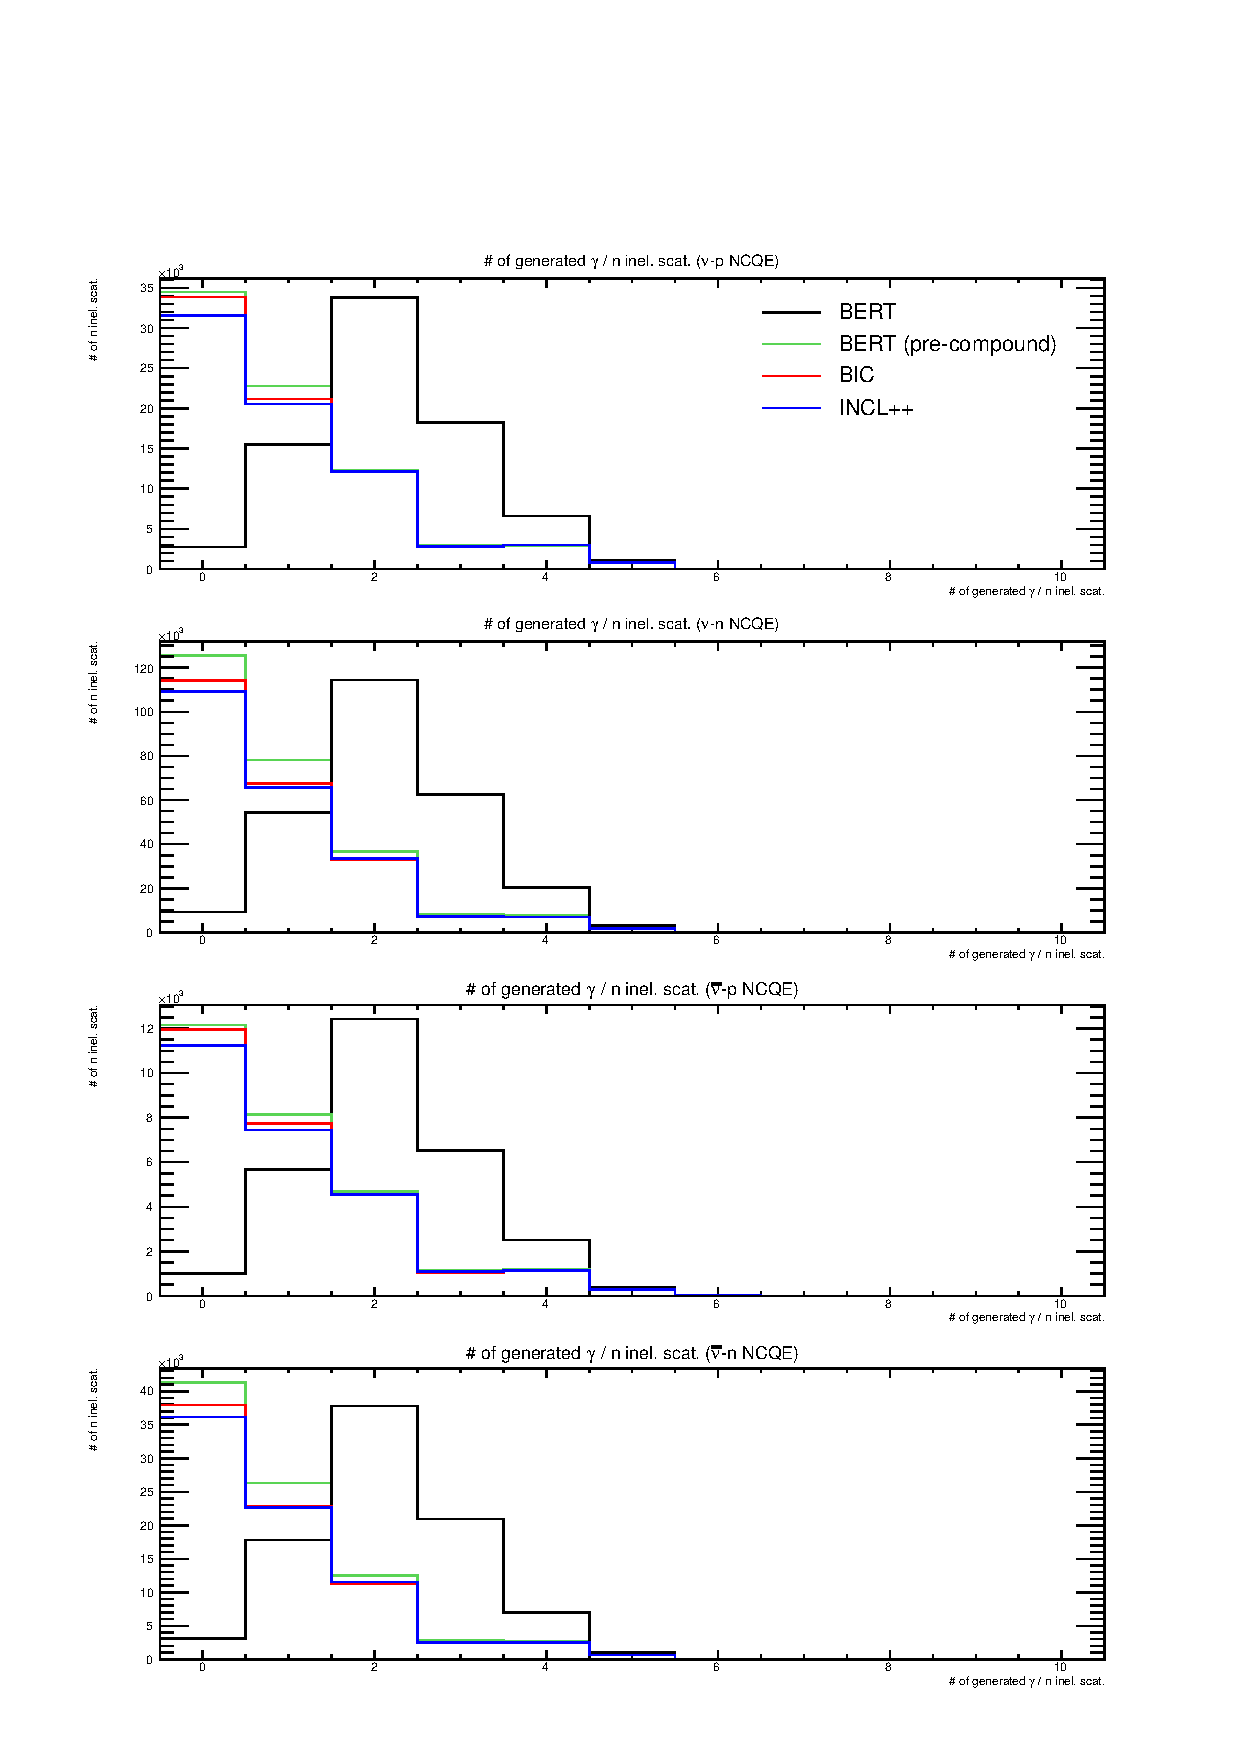
\includegraphics[width=16cm]{PDF/Secondary/Comparison_PreCompound/gamma/pdf1/NumSecIne}
	\caption[The number of generated gamma-rays per neutron inelastic scattering reaction]{
	The number of generated gamma-rays per neutron inelastic scattering reaction.
	Top, top middle, bottom middle, and bottom figure shows the case of neutrino-proton, neutrino-neutron, antineutrino-proton, and antineutrino-neutron NCQE reactions, respectively.
	Black, green, red, and blue line shows the case of BERT, BERT with the Geant4 pre-compound model, BIC, and INCL++, respectively.
	}\label{Others_gamma_NumSecIne}
\end{figure}

\begin{figure}[h]
	\centering
	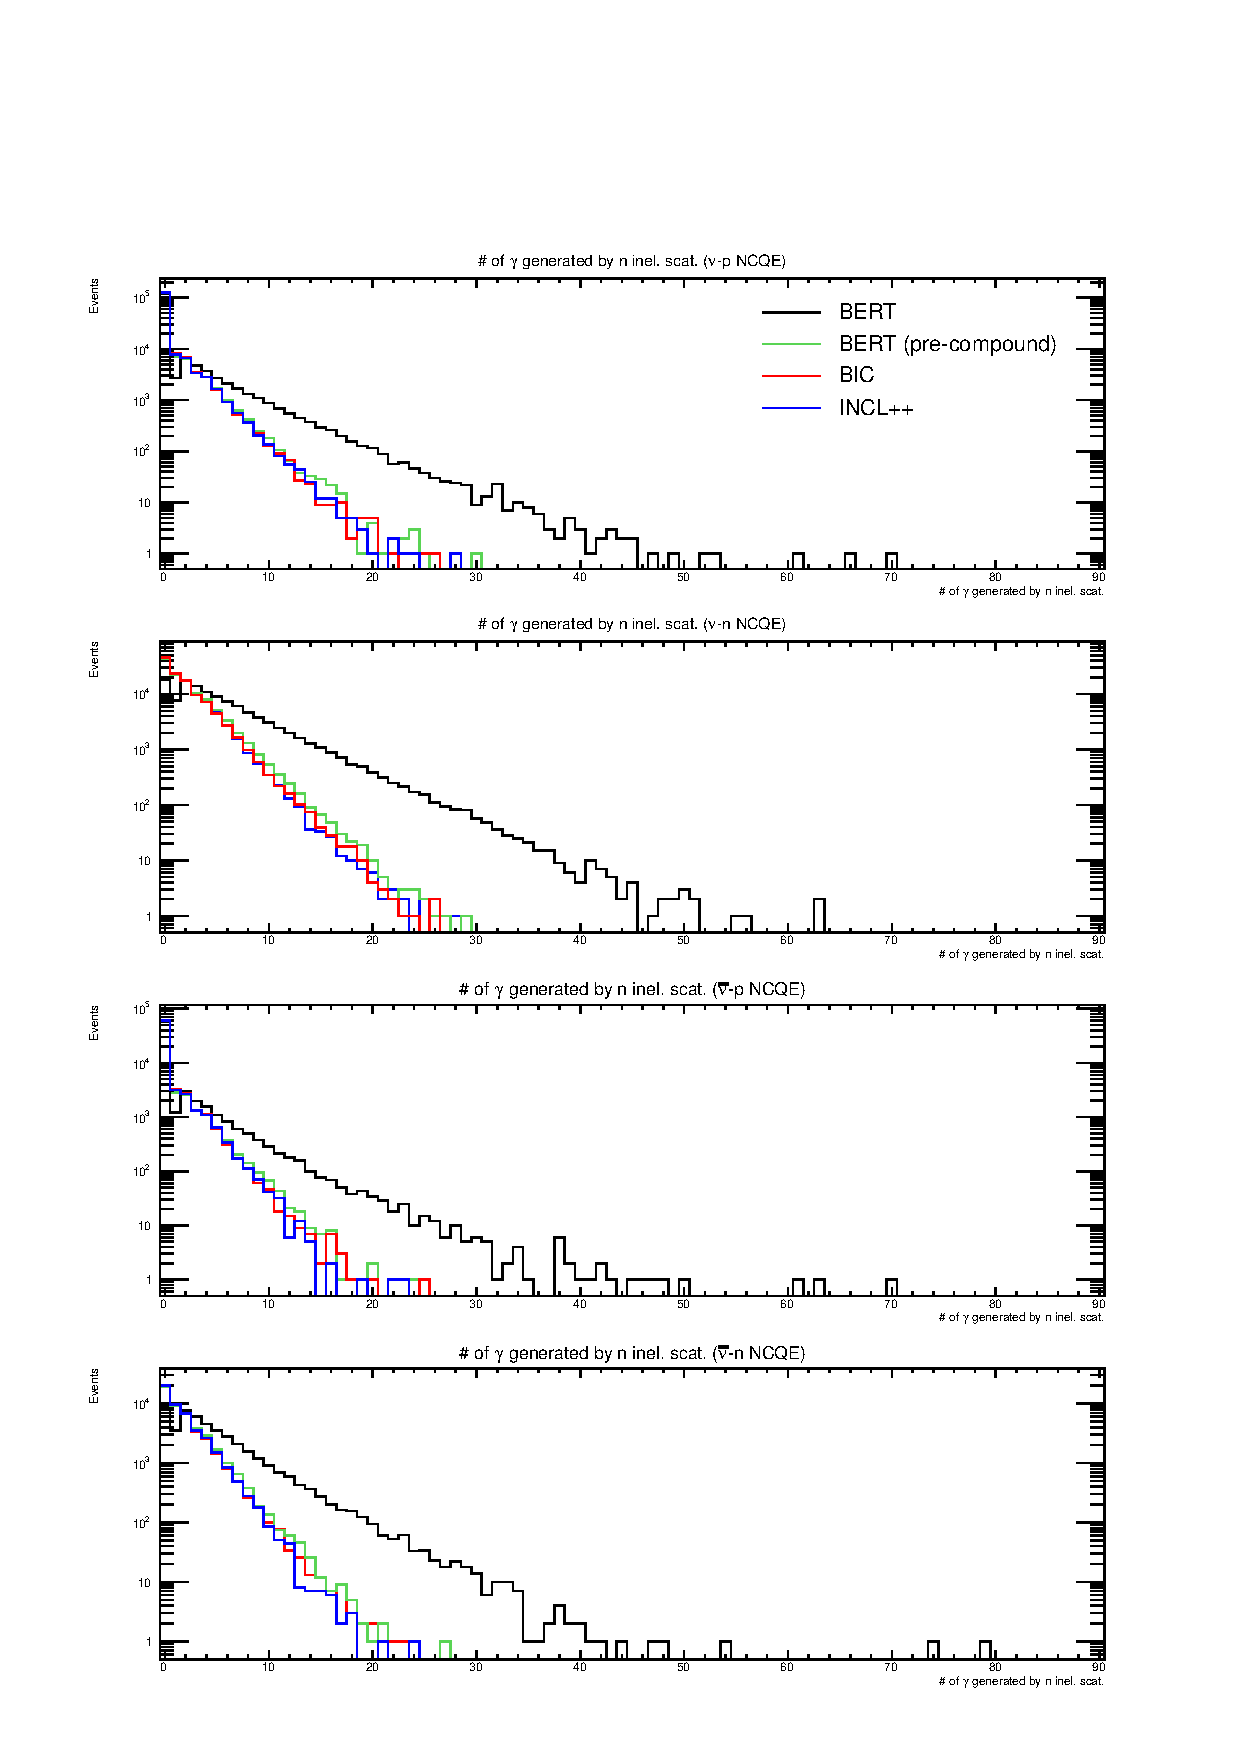
\includegraphics[width=16cm]{PDF/Secondary/Comparison_PreCompound/gamma/pdf1/Logy_NumSec}
	\caption[The number of gamma-rays generated by neutron inelastic scattering reactions]{
	The number of gamma-rays generated by neutron inelastic scattering reactions.
	Top, top middle, bottom middle, and bottom figure shows the case of neutrino-proton, neutrino-neutron, antineutrino-proton, and antineutrino-neutron NCQE reactions, respectively.
	Black, green, red, and blue line shows the case of BERT, BERT with the Geant4 pre-compound model, BIC, and INCL++, respectively.
	}\label{Others_gamma_Logy_NumSec}
\end{figure}

\begin{figure}[h]
	\centering
	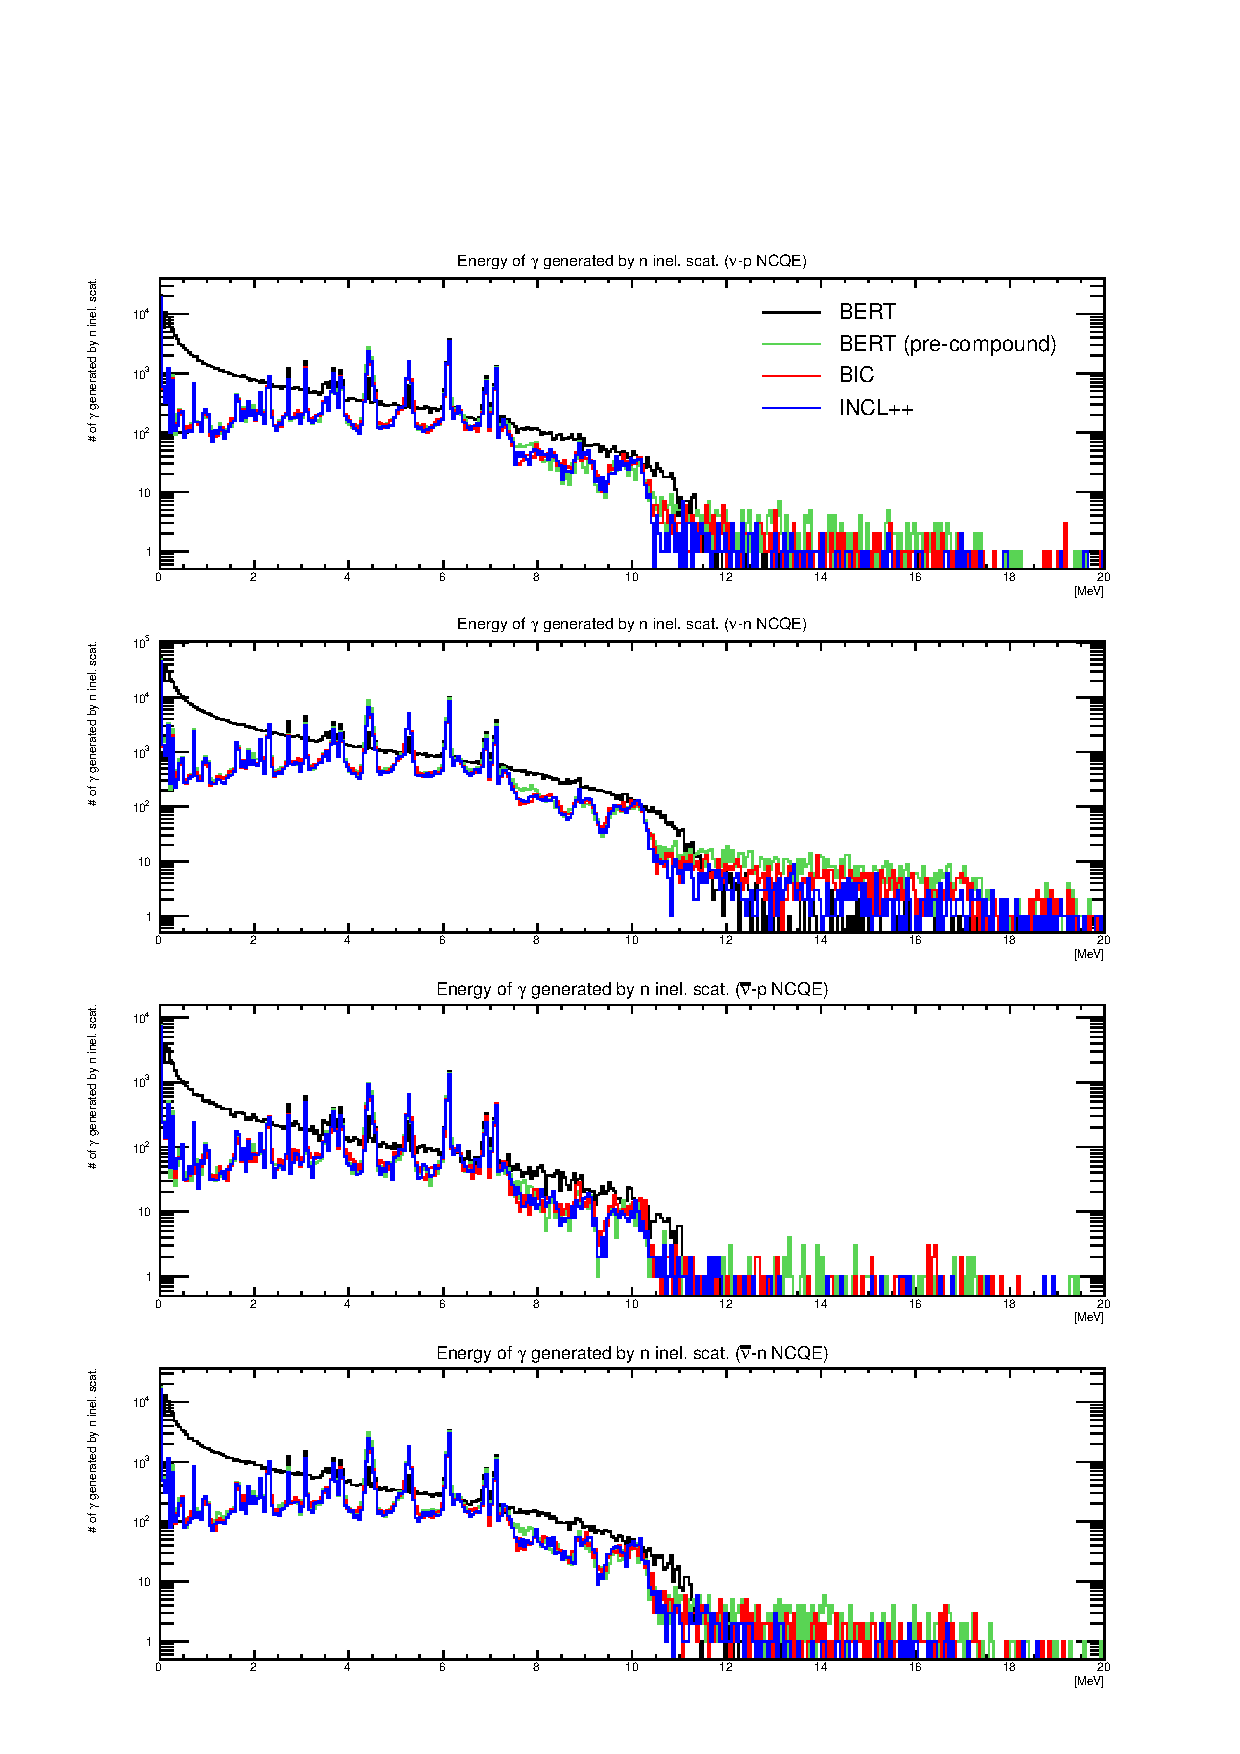
\includegraphics[width=16cm]{PDF/Secondary/Comparison_PreCompound/gamma/pdf1/Logy_EneSec}
	\caption[Energy of gamma-rays generated by neutron inelastic scattering reactions]{
	Energy of gamma-rays generated by neutron inelastic scattering reactions.
	Top, top middle, bottom middle, and bottom figure shows the case of neutrino-proton, neutrino-neutron, antineutrino-proton, and antineutrino-neutron NCQE reactions, respectively.
	Black, green, red, and blue line shows the case of BERT, BERT with the Geant4 pre-compound model, BIC, and INCL++, respectively.
	}\label{Others_gamma_Logy_EneSec}
\end{figure}

\begin{figure}[h]
	\centering
	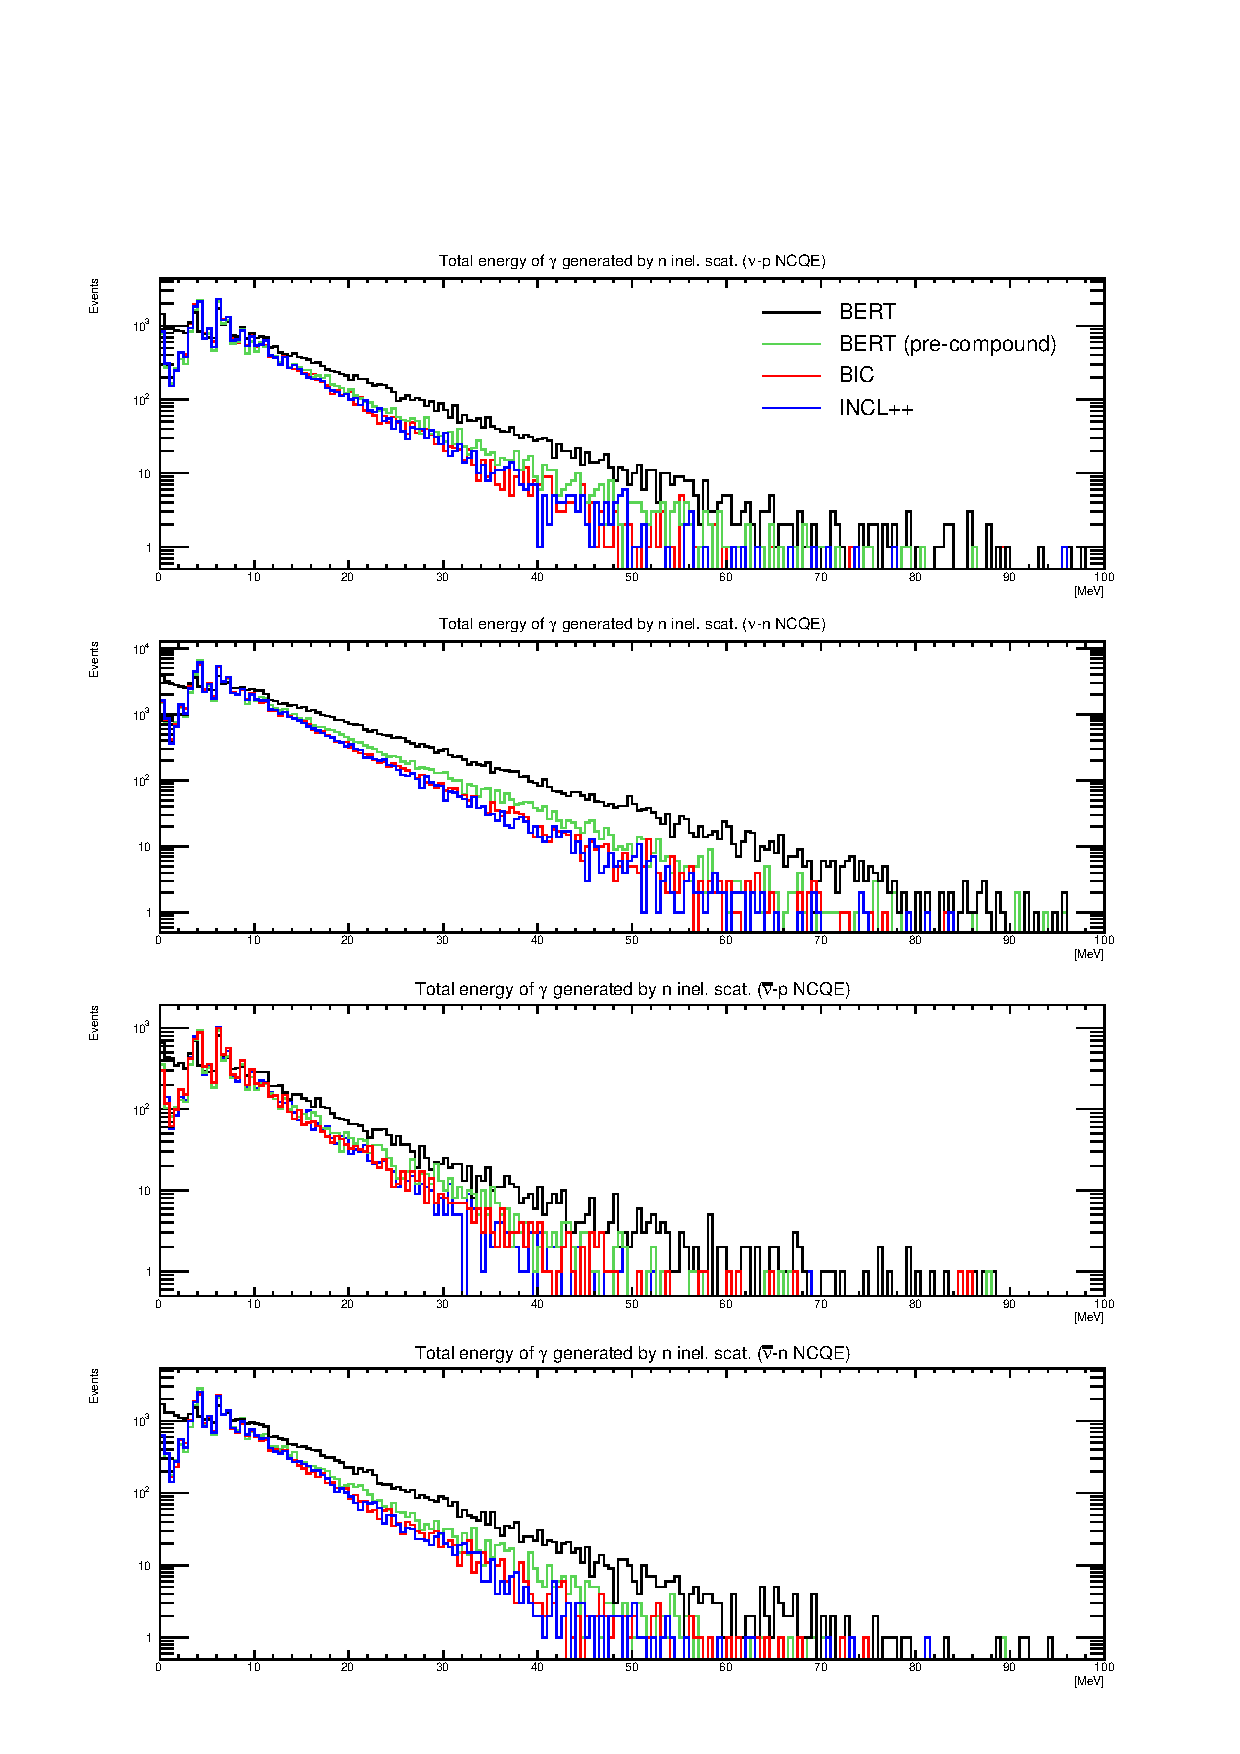
\includegraphics[width=16cm]{PDF/Secondary/Comparison_PreCompound/gamma/pdf1/Logy_TotEneSec}
	\caption[Total energy of gamma-rays generated by neutron inelastic scattering reactions]{
	Total energy of gamma-rays generated by neutron inelastic scattering reactions.
	Top, top middle, bottom middle, and bottom figure shows the case of neutrino-proton, neutrino-neutron, antineutrino-proton, and antineutrino-neutron NCQE reactions, respectively.
	Black, green, red, and blue line shows the case of BERT, BERT with the Geant4 pre-compound model, BIC, and INCL++, respectively.
	}\label{Others_gamma_Logy_TotEneSec}
\end{figure}

\begin{table}[h]
	\centering
	\caption[The number of neutrons generated by each process, the total number of neutrons and neutron captures, and the number of gamma-rays in the case of neutrino-proton NCQE reactions]{
	The number of neutrons generated by each process (top), the total number of neutrons and neutron captures (center), and the number of gamma-rays (bottom) in the case of neutrino-proton NCQE reactions.
	The numbers of primary neutrons and primary gamma-rays are common among secondary interaction models.
	}\label{Others_tab:pre_gamma_nuncqe_p}
	\vs
	\begin{tabular}{lrrrr} \hline \hline
		$\nu$-p NCQE (150,214~events)                       &    BERT &           BERT &     BIC &  INCL++ \\
		                                                    &         & (pre-compound) &         &         \\ \hline
		neutron inelastic scattering                        &  26,363 &         19,216 &  18,936 &  15,845 \\
		proton inelastic scattering                         &  21,253 &         17,614 &  22,485 &  20,159 \\
		$\pi^{+}$ inelastic scattering                      &     186 &            191 &     148 &     143 \\
		$\pi^{-}$ inelastic scattering                      &     137 &            128 &     161 &     122 \\
		$\mu^{-}$ capture                                   &       0 &              0 &       5 &       2 \\
		$\pi^{-}$ capture                                   &     757 &            704 &     864 &     837 \\
		gamma-nuclear interaction                           &      20 &             11 &      22 &      27 \\
		others                                              &      61 &             46 &      11 &     592 \\ \hline
		The number of generated neutrons                    &  48,777 &         37,910 &  42,632 &  37,727 \\ \hline
		The number of generated neutrons per event          &  0.3247 &         0.2524 &  0.2838 &  0.2512 \\ \hline \hline
		&&& \\ \hline \hline
		$\nu$-p NCQE (150,214~events)                       &    BERT &           BERT &     BIC &  INCL++ \\
		                                                    &         & (pre-compound) &         &         \\ \hline
		The number of primary neutrons                      &  67,105 &         67,105 &  67,105 &  67,105 \\
		The number of generated neutrons                    &  48,777 &         37,910 &  42,632 &  37,727 \\
		The total number of neutrons                        & 115,882 &        105,015 & 109,737 & 104,832 \\
		The number of neutron captures                      & 108,839 &         95,445 &  95,764 &  94,176 \\ \hline
		The number of primary neutrons per event            &  0.4467 &         0.4467 &  0.4467 &  0.4467 \\
		The number of generated neutrons per event          &  0.3247 &         0.2524 &  0.2838 &  0.2512 \\
		The total number of neutrons per event              &  0.7714 &         0.6991 &  0.7305 &  0.6979 \\
		The number of neutron captures per event            &  0.7246 &         0.6354 &  0.6375 &  0.6269 \\ \hline \hline
		&&& \\ \hline \hline
		$\nu$-p NCQE (150,214~events)                       &    BERT &           BERT &     BIC &  INCL++ \\
		                                                    &         & (pre-compound) &         &         \\ \hline
		The number of primary gamma-rays                    &  57,996 &         57,996 &  57,996 &  57,996 \\
		The number of n inel. scat.                         &  78,045 &         76,194 &  73,851 &  70,923 \\
		The number of gamma-rays per n inel. scat.          &  2.1776 &         0.9422 &  0.9477 &  0.9803 \\
		The number of gamma-rays by n inel. scat.           & 169,947 &         71,788 &  69,987 &  69,524 \\ \hline
		The number of primary gamma-rays per event          &  0.3861 &         0.3861 &  0.3861 &  0.3861 \\
		The number of n inel. scat. per event               &  0.5196 &         0.5072 &  0.4916 &  0.4721 \\
		The number of gamma-rays by n inel. scat. per event &  1.1314 &         0.4779 &  0.4659 &  0.4628 \\ \hline \hline
	\end{tabular}
\end{table}

\begin{table}[h]
	\centering
	\caption[The number of neutrons generated by each process, the total number of neutrons and neutron captures, and the number of gamma-rays in the case of neutrino-neutron NCQE reactions]{
	The number of neutrons generated by each process (top), the total number of neutrons and neutron captures (center), and the number of gamma-rays (bottom) in the case of neutrino-neutron NCQE reactions.
	The numbers of primary neutrons and primary gamma-rays are common among secondary interaction models.
	}\label{Others_tab:pre_gamma_nuncqe_n}
	\vs
	\begin{tabular}{lrrrr} \hline \hline
		$\nu$-n NCQE (116,031~events)                       &    BERT &           BERT &     BIC &  INCL++ \\
		                                                    &         & (pre-compound) &         &         \\ \hline
		neutron inelastic scattering                        & 110,049 &         82,016 &  76,597 &  66,201 \\
		proton inelastic scattering                         &   6,497 &          5,087 &   7,392 &   5,894 \\
		$\pi^{+}$ inelastic scattering                      &      90 &             62 &      76 &      70 \\
		$\pi^{-}$ inelastic scattering                      &     413 &            380 &     474 &     470 \\
		$\mu^{-}$ capture                                   &       1 &              9 &       8 &       7 \\
		$\pi^{-}$ capture                                   &   2,712 &          2,668 &   2,829 &   2,995 \\
		gamma-nuclear interaction                           &      30 &             20 &      23 &      20 \\
		others                                              &      93 &             77 &      29 &   1,103 \\ \hline
		The number of generated neutrons                    & 119,885 &         90,319 &  87,428 &  76,760 \\ \hline
		The number of generated neutrons per event          &  1.0332 &         0.7784 &  0.7535 &  0.6615 \\ \hline \hline
		&&& \\ \hline \hline
		$\nu$-n NCQE (116,031~events)                       &    BERT &           BERT &     BIC &  INCL++ \\
		                                                    &         & (pre-compound) &         &         \\ \hline
		The number of primary neutrons                      & 154,978 &        154,978 & 154,978 & 154,978 \\
		The number of generated neutrons                    & 119,885 &         90,319 &  87,428 &  76,760 \\
		The total number of neutrons                        & 274,863 &        245,297 & 242,406 & 231,738 \\
		The number of neutron captures                      & 255,807 &        217,113 & 205,968 & 202,607 \\ \hline
		The number of primary neutrons per event            &  1.3357 &         1.3357 &  1.3357 &  1.3357 \\
		The number of generated neutrons per event          &  1.0332 &         0.7784 &  0.7535 &  0.6615 \\
		The total number of neutrons per event              &  2.3689 &         2.1141 &  2.0891 &  1.9972 \\
		The number of neutron captures per event            &  2.2046 &         1.8712 &  1.7751 &  1.7461 \\ \hline \hline
		&&& \\ \hline \hline
		$\nu$-n NCQE (116,031~events)                       &    BERT &           BERT &     BIC &  INCL++ \\
		                                                    &         & (pre-compound) &         &         \\ \hline
		The number of primary gamma-rays                    &  59,612 &         59,612 &  59,612 &  59,612 \\
		The number of n inel. scat.                         & 263,957 &        258,553 & 230,736 & 224,076 \\
		The number of gamma-rays per n inel. scat.          &  2.1518 &         0.8437 &  0.8348 &  0.8524 \\
		The number of gamma-rays by n inel. scat.           & 567,986 &        218,135 & 192,614 & 191,012 \\ \hline
		The number of primary gamma-rays per event          &  0.5138 &         0.5138 &  0.5138 &  0.5138 \\
		The number of n inel. scat. per event               &  2.2749 &         2.2283 &  1.9886 &  1.9312 \\
		The number of gamma-rays by n inel. scat. per event &  4.8951 &         1.8800 &  1.6600 &  1.6462 \\ \hline \hline
	\end{tabular}
\end{table}

\begin{table}[h]
	\centering
	\caption[The number of neutrons generated by each process, the total number of neutrons and neutron captures, and the number of gamma-rays in the case of antineutrino-proton NCQE reactions]{
	The number of neutrons generated by each process (top), the total number of neutrons and neutron captures (center), and the number of gamma-rays (bottom) in the case of antineutrino-proton NCQE reactions.
	The numbers of primary neutrons and primary gamma-rays are common among secondary interaction models.
	}\label{Others_tab:pre_gamma_nubncqe_p}
	\vs
	\begin{tabular}{lrrrr} \hline \hline
		$\bar{\nu}$-p NCQE (70,695~events)                  &    BERT &           BERT &     BIC &  INCL++ \\
		                                                    &         & (pre-compound) &         &         \\ \hline
		neutron inelastic scattering                        &   8,730 &          6,184 &   6,227 &   5,343 \\
		proton inelastic scattering                         &   6,991 &          5,590 &   7,364 &   6,495 \\
		$\pi^{+}$ inelastic scattering                      &      55 &             53 &      51 &      63 \\
		$\pi^{-}$ inelastic scattering                      &      24 &             15 &      35 &      38 \\
		$\mu^{-}$ capture                                   &       0 &              0 &       0 &       0 \\
		$\pi^{-}$ capture                                   &     232 &            252 &     263 &     219 \\
		gamma-nuclear interaction                           &       6 &              7 &      10 &      11 \\
		others                                              &      16 &             17 &       1 &     168 \\ \hline
		The number of generated neutrons                    &  16,054 &         12,118 &  13,951 &  12,337 \\ \hline
		The number of generated neutrons per event          &  0.2271 &         0.1714 &  0.1973 &  0.1745 \\ \hline \hline
		&&& \\ \hline \hline
		$\bar{\nu}$-p NCQE (70,695~events)                  &    BERT &           BERT &     BIC &  INCL++ \\
		                                                    &         & (pre-compound) &         &         \\ \hline
		The number of primary neutrons                      &  28,958 &         28,958 &  28,958 &  28,958 \\
		The number of generated neutrons                    &  16,054 &         12,118 &  13,951 &  12,337 \\
		The total number of neutrons                        &  45,012 &         41,076 &  42,909 &  41,295 \\
		The number of neutron captures                      &  42,327 &         37,208 &  37,587 &  37,208 \\ \hline
		The number of primary neutrons per event            &  0.4096 &         0.4096 &  0.4096 &  0.4096 \\
		The number of generated neutrons per event          &  0.2271 &         0.1714 &  0.1973 &  0.1745 \\
		The total number of neutrons per event              &  0.6367 &         0.5810 &  0.6070 &  0.5841 \\
		The number of neutron captures per event            &  0.5987 &         0.5263 &  0.5317 &  0.5263 \\ \hline \hline
		&&& \\ \hline \hline
		$\bar{\nu}$-p NCQE (70,695~events)                  &    BERT &           BERT &     BIC &  INCL++ \\
		                                                    &         & (pre-compound) &         &         \\ \hline
		The number of primary gamma-rays                    &  26,774 &         26,774 &  26,774 &  26,774 \\
		The number of n inel. scat.                         &  28,557 &         27,634 &  26,734 &  25,778 \\
		The number of gamma-rays per n inel. scat.          &  2.1770 &         0.9886 &  0.9731 &  1.0061 \\
		The number of gamma-rays by n inel. scat.           &  62,170 &         27,319 &  26,014 &  25,936 \\ \hline
		The number of primary gamma-rays per event          &  0.3787 &         0.3787 &  0.3787 &  0.3787 \\
		The number of n inel. scat. per event               &  0.4039 &         0.3909 &  0.3782 &  0.3646 \\
		The number of gamma-rays by n inel. scat. per event &  0.8794 &         0.3864 &  0.3680 &  0.3669 \\ \hline \hline
	\end{tabular}
\end{table}

\begin{table}[h]
	\centering
	\caption[The number of neutrons generated by each process, the total number of neutrons and neutron captures, and the number of gamma-rays in the case of antineutrino-neutron NCQE reactions]{
	The number of neutrons generated by each process (top), the total number of neutrons and neutron captures (center), and the number of gamma-rays (bottom) in the case of antineutrino-neutron NCQE reactions.
	The numbers of primary neutrons and primary gamma-rays are common among secondary interaction models.
	}\label{Others_tab:pre_gamma_nubncqe_n}
	\vs
	\begin{tabular}{lrrrr} \hline \hline
		$\bar{\nu}$-n NCQE (46,344~events)                  &    BERT &           BERT &     BIC &  INCL++ \\
		                                                    &         & (pre-compound) &         &         \\ \hline
		neutron inelastic scattering                        &  32,887 &         23,921 &  22,822 &  19,638 \\
		proton inelastic scattering                         &   1,554 &          1,322 &   1,871 &   1,492 \\
		$\pi^{+}$ inelastic scattering                      &      18 &             16 &      22 &       9 \\
		$\pi^{-}$ inelastic scattering                      &      64 &             69 &     115 &      92 \\
		$\mu^{-}$ capture                                   &       9 &              0 &       2 &       3 \\
		$\pi^{-}$ capture                                   &     520 &            531 &     592 &     642 \\
		gamma-nuclear interaction                           &       8 &              4 &       6 &       3 \\
		others                                              &      26 &             29 &       4 &     301 \\ \hline
		The number of generated neutrons                    &  35,086 &         25,892 &  25,434 &  22,180 \\ \hline
		The number of generated neutrons per event          &  0.7571 &         0.5587 &  0.5488 &  0.4786 \\ \hline \hline
		&&& \\ \hline \hline
		$\bar{\nu}$-n NCQE (46,344~events)                  &    BERT &           BERT &     BIC &  INCL++ \\
		                                                    &         & (pre-compound) &         &         \\ \hline
		The number of primary neutrons                      &  59,794 &         59,794 &  59,794 &  59,794 \\
		The number of generated neutrons                    &  35,086 &         25,892 &  25,434 &  22,180 \\
		The total number of neutrons                        &  94,880 &         85,686 &  85,228 &  81,974 \\
		The number of neutron captures                      &  88,373 &         75,952 &  71,768 &  71,492 \\ \hline
		The number of primary neutrons per event            &  1.2902 &         1.2902 &  1.2902 &  1.2902 \\
		The number of generated neutrons per event          &  0.7571 &         0.5587 &  0.5488 &  0.4786 \\
		The total number of neutrons per event              &  2.0473 &         1.8489 &  1.8390 &  1.7688 \\
		The number of neutron captures per event            &  1.9069 &         1.6389 &  1.5486 &  1.5426 \\ \hline \hline
		&&& \\ \hline \hline
		$\bar{\nu}$-n NCQE (46,344~events)                  &    BERT &           BERT &     BIC &  INCL++ \\
		                                                    &         & (pre-compound) &         &         \\ \hline
		The number of primary gamma-rays                    &  23,678 &         23,678 &  23,678 &  23,678 \\
		The number of n inel. scat.                         &  87,695 &         86,394 &  77,698 &  76,027 \\
		The number of gamma-rays per n inel. scat.          &  2.1629 &         0.8611 &  0.8529 &  0.8782 \\
		The number of gamma-rays by n inel. scat.           & 189,679 &         74,391 &  66,271 &  66,765 \\ \hline
		The number of primary gamma-rays per event          &  0.5109 &         0.5109 &  0.5109 &  0.5109 \\
		The number of n inel. scat. per event               &  1.8923 &         1.8642 &  1.6765 &  1.6405 \\
		The number of gamma-rays by n inel. scat. per event &  4.0928 &         1.6052 &  1.4300 &  1.4406 \\ \hline \hline
	\end{tabular}
\end{table}





\clearpage
\subsection{Measurement of NCQE cross section in SK-Gd}\label{App_NCQE}
\vs\hs
Other distributions related to Section~\ref{Sec_NCQE} are summarized here.

\begin{figure}[H]
	\centering
	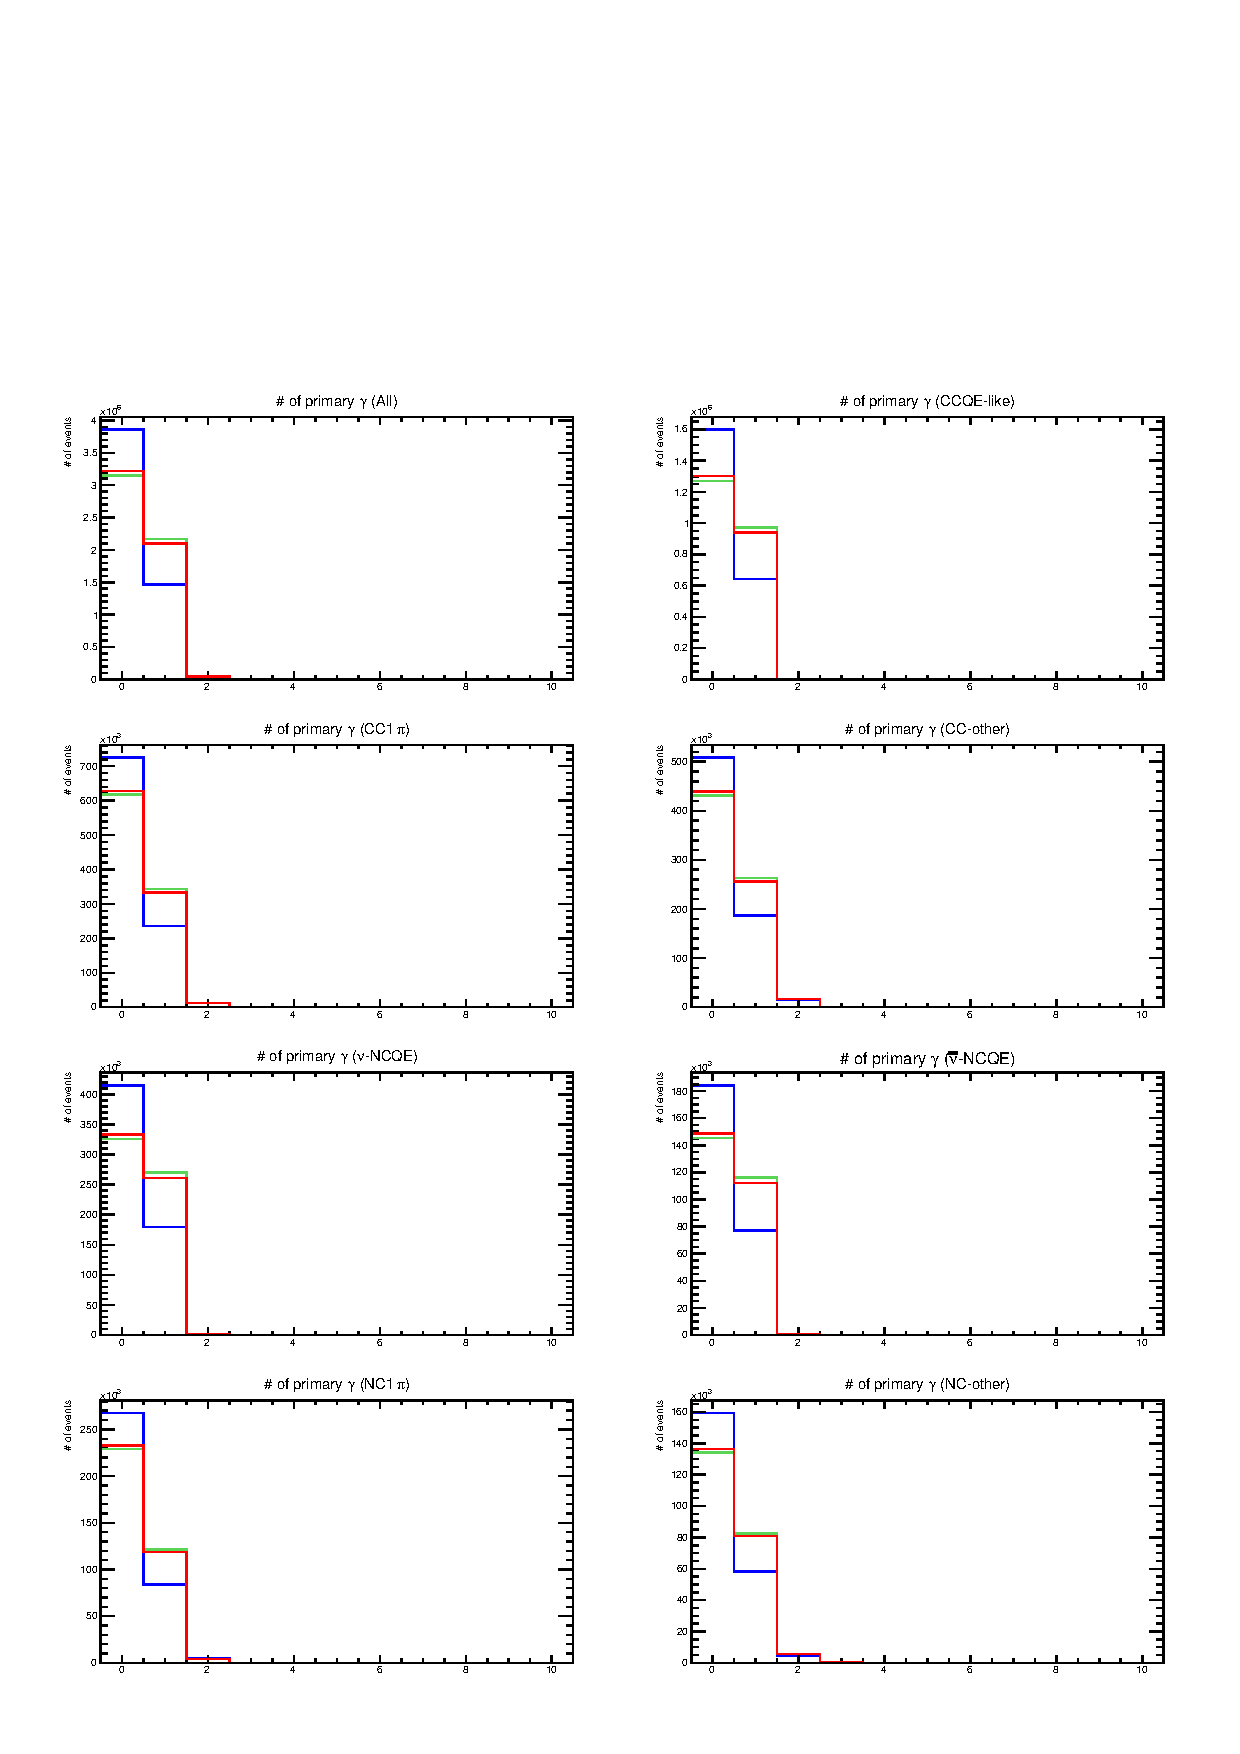
\includegraphics[width=16cm]{PDF/NEUT/Comparison/gamma/NumPri}
	\caption[The comparison of the number of gamma-rays generated by neutrino-nucleus interaction]{
	The comparison of the number of gamma-rays generated by neutrino-nucleus interaction.
	The red line shows the case of including \textit{others} state into $(s_{1/2})^{-1}$ state.
	The blue line shows the case of including \textit{others} state into $(p_{1/2})^{-1}$ state.
	The green line shows the case of increasing $(p_{3/2})^{-1}$ state by 5.4\%.
	These figures were made using 500 years' worth of atmospheric neutrino events.
	}\label{Comp_gammaNumPri}
\end{figure}

\begin{figure}[h]
	\centering
	\includegraphics[width=16cm]{PDF/NEUT/Comparison/gamma/EnePri}
	\caption[The comparison of energy of gamma-rays generated by neutrino-nucleus interaction]{
	The comparison of energy of gamma-rays generated by neutrino-nucleus interaction.
	The red line shows the case of including \textit{others} state into $(s_{1/2})^{-1}$ state.
	The blue line shows the case of including \textit{others} state into $(p_{1/2})^{-1}$ state.
	The green line shows the case of increasing $(p_{3/2})^{-1}$ state by 5.4\%.
	These figures were made using 500 years' worth of atmospheric neutrino events.
	}\label{Comp_gammaEnePri}
\end{figure}

\begin{figure}[h]
	\centering
	\includegraphics[width=16cm]{PDF/NEUT/Comparison/neutron/NumPri}
	\caption[The comparison of the number of neutrons generated by neutrino-nucleus interaction]{
	The comparison of the number of neutrons generated by neutrino-nucleus interaction.
	The red line shows the case of including \textit{others} state into $(s_{1/2})^{-1}$ state.
	The blue line shows the case of including \textit{others} state into $(p_{1/2})^{-1}$ state.
	The green line shows the case of increasing $(p_{3/2})^{-1}$ state by 5.4\%.
	These figures were made using 500 years' worth of atmospheric neutrino events.
	}\label{Comp_neutronNumPri}
\end{figure}

\begin{figure}[h]
	\centering
	\includegraphics[width=16cm]{PDF/NEUT/Comparison/neutron/LogEnePri}
	\caption[The comparison of energy of neutrons generated by neutrino-nucleus interaction]{
	The comparison of energy of neutrons generated by neutrino-nucleus interaction.
	The red line shows the case of including \textit{others} state into $(s_{1/2})^{-1}$ state.
	The blue line shows the case of including \textit{others} state into $(p_{1/2})^{-1}$ state.
	The green line shows the case of increasing $(p_{3/2})^{-1}$ state by 5.4\%.
	These figures were made using 500 years' worth of atmospheric neutrino events.
	}\label{Comp_neutronLogEnePri}
\end{figure}





\newpage

